%$RUN*$ pdflatex ${FILE} &&  pdflatex ${FILE} &&  acroread -openInNewWindow ${BASENAME}.pdf

\documentclass{article}
\usepackage{hyperref}
\usepackage{color}
\usepackage{multirow}
\usepackage{graphics}

\newcommand{\beq}{\begin{equation}}
\newcommand{\eeq}{\end{equation}}
\newcommand{\beqa}{\begin{eqnarray}}
\newcommand{\eeqa}{\end{eqnarray}}
\newcommand{\bvb}{\begin{verbatim}}
\newcommand{\evb}{\end{verbatim}}
\newcommand{\beqann}{\begin{eqnarray*}}
\newcommand{\eeqann}{\end{eqnarray*}}
\newcommand{\nn}{\mbox{${\nonumber}$}}
\newcommand{\labeq}[1]{\label{eq:#1}}
\newcommand{\refeq}[1]{(\ref{eq:#1})}
\newcommand{\tc}[1]{\addcontentsline{toc}{subsection}{#1}}
\newcommand{\TCC}[1]{\medskip

\addcontentsline{toc}{subsubsection}{#1}
\noindent{\bf {#1}.}}
	
\newcommand{\tcc}[1]{\addcontentsline{toc}{subsubsection}{#1}}
\title{XPPAUT5.41 -- the differential equations tool}
\author{Bard Ermentrout}
\begin{document}
\maketitle
\tableofcontents
\newpage
\section{Introduction} XPP (XPPAUT is another name; I will use the two
interchangeably)
  is a tool for solving differential
equations,
 difference 
equations, delay equations, functional equations, boundary value
problems, and stochastic equations. 
 It evolved 
from a chapter written by John Rinzel and myself on the qualitative
 theory of nerve membranes and eventually became a commercial product
 for MSDOS computers called PHASEPLANE.  It is now available as a
program running
 under
 X11 and UNIX.  

 The code 
brings together a number of useful algorithms and is extremely portable. 
 All the graphics and interface are written completely in Xlib which explains 
the somewhat idiosyncratic and primitive widgets interface.  

XPP contains the code for the popular bifurcation
program, AUTO.  Thus, you can switch back and forth between XPP and
AUTO, using the values of one program in the other and vice-versa.  I
have put a ``friendly'' face on AUTO as well.  You do not need to know
much about it to play around with it.

XPP has the capabilities for handling up to 5000 differential equations. 
 There are solvers for delay and stiff differential equations a well as
 some code for boundary value problems.  Difference equations are also
 handled.  Up to 10 graphics windows can be visible at once and a variety
 of color combinations is supported.  PostScript/SVG output
 is supported.  Post processing is easy and includes the ability to make
 histograms, FFTs and applying functions to columns of your data.
Equilibria
 and linear stability as well as one-dimensional invariant sets can be
 computed.  Nullclines and flow fields aid in the qualitative understanding
 of two-dimensional models.  Poincare maps and equations on cylinders and
 tori are also supported.  Some useful averaging theory tricks and various
 methods for dealing with coupled oscillators are included primarily because
 that is what I do for a living. Equations with Dirac delta functions
are allowable.

There is an animation package that allows you to
create animated versions of your simulations, such as a little
pendulum moving back and forth or lamprey swimming. The new window for
animations is produced by invoking the {\tt (V)iew axes} {\tt (T)oon}
menu item.  See section \ref{toon} for complete info.

 
I will assume that you are well versed in the theory of ordinary differential
 equations although you need not be to use the program.  
There are a number of useful features designed for people who use
dynamical systems to {\em model} their experiments.  There is a
curve-fitter based on the Marquardt-Levenberg algorithm which lets you
fit data points to the solutions to dynamical systems.  
Gnuplot-like graphics and
support for some graphics objects such as text, arrows, and
pointers are part of the package. You can also import bifurcation
curves as part of your graphs.
 It is possible to automatically generate ``movies'' of
three-dimensional views of attractors or parametric changes in the
attractor as some parameters vary.    I have
also included a small preprocessing utility that allows one to create
files for large systems of coupled equations. 

There are a number of other such programs available, but they all seem to
 require that your problems be compiled before using them.  XPP does not;
 I have devised a simple and fairly fast formula compiler that is based
 on the idea of the inner interpretor used in the language FORTH (which
 remains my first love as far as language is concerned)  Fear not, the
 differential equations and boundary conditions and other formulae are
 written in usual algebraic notation.  However, in order to run big
problems very quickly, I have written the code so that it is possible
to create a library that can be linked to your problem and thus create
a binary with the right-hand sides compiled.  This can run much faster
than the parsed code.  See the notes on this at the end of the
document. 



XPP has been compiled on most UNIX machines and works fine now on Windows, Macs, and Linux.
Building XPP requires only the standard C compiler,
 and Xlib.  Look at the any README files that come with the
distribution for solutions to common compilation problems.



The basic unit for XPP is a single ASCII file (hereafter called an ODE
file) that has the equations, parameters,
 variables, boundary conditions, and functions for your model. You can
also include numerical parameters such as time step size and method of
integration although these can also be changed within the program.
The graphics and postprocessing are all done within
 the program using the mouse and various menus and buttons.  The impatient
 user should look at some sample {\tt *.ode} files instead of actually reading 
the documentation.  There are many command line arguments and options that can be added to set up numerics. There is also a resource file .xpprc that you can add to your home directory.  Look at xpp\_sum.pdf for details on this.  The documentaion here is pretty incomplete, but covers much of the basics. There is a book from SIAM available and you can also look at the included tree.pdf file that gives a description of {\em every} command.

 
\addcontentsline{toc}{subsection}{Interface}
\begin{center}
{\Large Notes on the Interface }
\end{center}
The interface is pretty simplistic and idiosyncratic.  Since the source code is available, if you really hate it, you can rewrite it.  You can customize fonts etc (see xpp\_sum.pdf).  
The text editing is also somewhat restricted.  There is  no cut
and paste.  However,
one can use the {\tt Home,End} keys to move the text cursor to the
beginning and end of the line.  The left and right arrow keys let you
move back and forth.  You can  insert or delete text at any point.
{\bf NOTE:} Be careful with the BackSpace and Delete keys as on some
systems they are mapped differently.  One of them causes the whole
line to be erased and the other just erases a single character.
Almost every command has a keyboard shortcut.  These are given below.


\tc{Disclaimer}
\begin{center} 

\Large Disclaimer \\

\end{center}

XPP is distributed as is.  The author makes no claims as to the performance
 of the program.  Anyone is allowed to modify and distribute XPP as long as
 the original code is also made available. See the LICENSE file for the full caveats.  

\tc{Acknowledgments}
\begin{center}
Acknowledgements
\end{center}
Artie Sherman, John Rinzel for many suggestions. Daniel Dougherty and Robert McDougal for contribution actual code!  Also Sebius Doedel for making AUTO available.  I want to also thank Bart Oldmann for some pointers on the porting of the most recent AUTO version.

Please let me know of any bugs or other stuff that you'd like to see
incorporated into XPP.  I will usually fix them quickly.  
  
My EMAIL address is bard@pitt.edu.
\tc{World Wide Web Tutorial}
\begin{center}
{\bf NOTE}
\end{center}
The easiest way to get a thorough understanding of the program as well
as a short tutorial in dynamical systems is to use the World Wide Web
tutorial which can be accessed from my home page at 
http://www.pitt.edu/$\equiv$phase. This tutorial is geared toward
computational neuroscientists (in the choice of problems) but provides
a fairly detailed introduction to the program.  
\subsection{Environment variables.}
While you can make a file in your home
directory called {\tt .xpprc} which contains a list of commonly used
options, XPP also uses some environment variables.  Note, on Windows computers the default
 home directory is taken to be a user's Desktop folder.

The environment variables which XPP uses are:
\begin{description}
	\item{\ttfamily\textbf{XPPBROWSER}}
              Web browser to view documentation (e.g. /usr/bin/firefox)
	\item{\ttfamily\textbf{XPPEDITOR}}
              Text editor to view/edit documentation (e.g. /usr/bin/gedit)
	\item{\ttfamily\textbf{XPPHELP}}
              Path to  the  XPPAUT  documentation  file  $<$xpphelp.html$>$\\  (e.g.
              /usr/share/doc/xppaut/html/xpphelp.html)
	\item{\ttfamily\textbf{XPPSTART}}
              File browser will open to the specified path. This may be useful
              in  an instructional setting to point to a mapped drive containing 
	      course materials or an NFS file share.
       
\end{description}


%\begin{verbatim}
%export XPPHELP=/home/bard/xppnew/help/xpphelp.html
%export BROWSER=/usr/bin/netscape
%\end{verbatim}

On Mac/Linux/Unix systems, these environment variables are typically set within a user's .bashrc file using export commands.  For example:
{\color{red}\begin{verbatim}
        export XPPHELP=/usr/share/doc/xppaut/html/xpphelp.html
        export XPPBROWSER=/usr/bin/firefox
        export XPPEDITOR=/usr/bin/nedit
        export XPPSTART=/usr/share/doc/xppaut/examples/ode
\end{verbatim}}

When I run XPP on {Windows}, I run the following bat file (xppaut.bat) which serves
to set various environment variables:
%\begin{verbatim}
%set BROWSER=c:\Program Files\Netscape\Communicator\Program\netscape.exe
%set XPPHELP=c:\xppall\help\xpphelp.html
%set DISPLAY=127.0.0.1:0.0
%set HOME=c:\xppall
%xppaut %1 %2 %3
%\end{verbatim}
{\color{red}
\begin{verbatim}
:: Specify location of where you want your .xpprc to be.
:: For most Windows users their Desktop is probably a safe bet.
set HOME=%HOMEDRIVE%%HOMEPATH%\Desktop
:: Change path to your favorite browser
set XPPBROWSER=c:/Program Files/Netscape/Communicator/Program/netscape.exe
set XPPHELP=c:/xppall/help/xpphelp.html
set DISPLAY=127.0.0.1:0.0

:: Might want to change this to JEdit or whatever text editor you use.
:: set XPPEDITOR=c:/Windows/notepad
set XPPEDITOR=notepad++

:: You may want to set XPPSTART to your research or course directory
set XPPSTART=c:/xppall/ode

set argC=0
for %%x in (%*) do Set /A argC+=1
IF %argC%==0 (c:/xppall/xppaut) ELSE (c:/xppall/xppaut %1 %2 %3)
pause
\end{verbatim}}

Here is my {\tt .xpprc} file:
{\color{red}\begin{verbatim}
# xpprc file
@ but=quit:fq
@ maxstor=50000,bell=0
@ meth=qualrk,tol=1e-6,atol=1e-6
# thats it
\end{verbatim}}

\section{ODE Files}

{\bf NOTE.}  {\em Pre 1992, XPP used a different form for ODE files. I no longer document them}  A command line option lets you convert old-style to
new style format.


ODE files are ASCII readable files that the XPP parser reads to create
 machine usable code. Lines can be continued with the standard
backslash character, however, the total length of any line cannot
exceed 1000 characters.

\bigskip
\tc{Example}
{\bf Example.} 
I will start with a very simple example to get you up and running. The
model is the periodically driven Fitzhugh-Nagumo equation:
\beqa
dv/dt &=& f(v)-w+s(t)+I_0 \\
dw/dt &=& \epsilon(v-\gamma w) \\
f(v) &=& v(1-v)(v-a) \\
s(t) &=& \alpha \sin \omega t
\eeqa

Here is the ODE file:
\begin{verbatim}
# Forced Fitzhugh-Nagumo fhn.ode 
dv/dt = f(v)-w+s(t)+I_0
dw/dt = eps*(v-gamma*w)
f(v)=v*(1-v)*(v-a)
s(t)=al*sin(omega*t)
param a=.25,eps=.05,gamma=1,I_0=.25
param al=0,omega=2
@ total=100,dt=.2,xhi=100
done
\end{verbatim}

The file is pretty self-explanatory.  The first line cannot contain a
number as its first character (this makes the parser think that the
format of the ODE file is the old style.)  The last line should be the
word ``done.''  The names of all parameters must be declared with
optional values (the default sets them to 0.) There can be as many as
you can fit on each line (up to 2000 parameters) but they must be
separated by commas or spaces and the ``='' sign must have {\em no} spaces on
either side of it.  

You could optionally include initial data by adding either of the
following sets of lines to the file:
\begin{verbatim}
init v=.25,w=.3
\end{verbatim}
or
\begin{verbatim}
v(0)=.25
w(0)=.3
\end{verbatim}

As you have probably guessed, comments have the form:
\begin{verbatim}
# This is a comment
\end{verbatim}

The ``@'' sign tells XPP that you want to preset some of the internal
parameters for numerical integration and graphing, AUTO, etc. Please put a space after the ``@'' on each line or it wont work.
  In this case, we have told XPP
to integrate the equations until t=100 with a timestep of 0.25 and to
set the high value for the x-axis to 100.  You can, of course, change
all these internal options from within XPP; this provides an easy way
``set'' up the problem for ``one-button'' operation. 

\tc{Quick exploration.}
\begin{center} {\Large Quick exploration} \end{center}

Once you have written an ODE file, you can run XPP by typing
\begin{verbatim}
xpp ffhn.ode
\end{verbatim}
where {\tt ffhn.ode} is the filename you created.  You may have to
type
\begin{verbatim}
xppaut ffhn.ode
\end{verbatim}
depending on what you named the program. (The distributed source
produces a binary called {\tt xppaut} , but I usually create a shell
script called {\tt xpp} that contains the following line
\begin{verbatim}
xppaut $1 -xorfix
\end{verbatim}
thus alleviating problems my display has with the exclusive or drawing
required for ``zooming'' in and other things.)
Several distributions such as for the Mac and Windows let you drag and drop.

When you type one of the above lines, then the program fires up. It
reads the ODE file and if there are any errors, it reports them and
returns to the command line.  Assuming you haven't written the ODE
file wrong (which you shouldn't have since it is included in the
source) you should get the main window.  Depending on your X windows
system, the other windows may or may not be iconified.  Almost all
command have keyboard shortcuts which are either the first letter of
the command or the letter in parentheses or capitalized. Thus, you can
oeither use the mouse to click on the command or you can use the
keyboard to choose the command.  To solve the differential equation
with the current parameters, click on {\tt Initialconds} and then {\tt
Go}. You will see the variable $V(t)$ plotted across the screen as a
function of time.  (Instead of using the mouse, you could type {\tt I
G} as a keyboard shortcut.)  Click on {\tt Xivst}.  When the prompt
comes up backspace over {\tt V}, and type in {\tt w} and {\tt Enter.}
The variable $w$ will be plotted versus time.  Note that the vertical
axis of the window is automatically adjusted.  Click on {\tt Viewaxes}
to choose the view and when the new window pops up fill it in as follows:
\begin{itemize} {\tt
\item X-axis: V
\item Y-axis: W
\item Xmin: -.5
\item Ymin: 0
\item Xmax: 1.5
\item Ymax: 1
\item Xlabel: V
\item Ylabel: w
}
\end{itemize}
and then click on {\tt Ok.}  The phase-plane will be drawn showing a
limit cycle. Click {\tt Nullclines} and then {\tt New} to draw the
nullclines. Click {\tt Text,etc} then {\tt Text} and type in
``V-nullcline'' followed by {\tt Enter} at the prompt.  Accept the
defaults for text size and font by typing {\tt Enter} twice.  Move the
mouse pointer to the cubic-like curve and click the button.  The text
should appear on the screen.  Repeat this but type in ``w-nullcline''
for the text.  Click {\tt Graphic stuff} and then {\tt Postscript}.
Accept the defaults and a hardcopy postscript file will be produced
which you can view or printout on an appropriate printer.  Click {\tt
File} and then {\tt Quit} and answer {\tt Yes} to exit XPP.  

A much more extensive tutorial is available on the World Wide Web (see
above). This document is mainly a reference to all the features (bugs
:) of XPP.

 
\begin{center}
{\Large ODE File format }
\end{center}
\tc{ODE File format} 
ODE files consist of ascii readable text which XPP uses to describe
the program it wants to solve.  The line length is limited to 256
characters total. Individual lines can be continued with the UNIX
backslash character, $\backslash.$ ODE files have any combination of the
following lines.  The order is not too important but can matter (see
below).
 

\begin{verbatim}
# comment line - name of file, etc   
...
#include <filename>
...
d<name>/dt=<formula>
<name>'=<formula>
...
<name>(t)=<formula>
...
volt <name>=<formula>
...
<name>(t+1)=<formula>
...
markov <name> <nstates>
{t01} {t02} ... {t0k-1}
{t10} ...
...
{tk-1,0} ...
...
aux <name>=<formula>
...
<name>=<formula>
...
parameter <name1>=<value1>,<name2>=<value2>, ...
...
!<name>=<formula>
...
wiener <name1>, <name2>, ...
...
number <name1>=<value1>,<name2>=<value2>, ...
...
<name>(<x1>,<x2>,...,<xn>)=<formula>
...
table <name> <filename>
...
table <name> % <npts> <xlo> <xhi> <function(t)>
...
global sign {condition} {name1=form1;...}
...
init <name>=<value>,...
...
<name>(0)=<value> or <expr>
...
bdry <expression>
...
%[i1 .. i2]
...
%
command[i1..i2] ...
...
name[i1..i2] ...
...
0= <expression>
...
solv <name>=<expression>
...
special <name>=conv(type,npts,ncon,wgt,rootname)
	       fconv(type,npts,ncon,wgt,rootname,root2,function)
	       sparse(npts,ncon,wgt,index,rootname)
               fsparse(npts,ncon,wgt,index,rootname,root2,function)
               mmult(n,m,w,root)
               fmmult(n,m,w,root1,root2,function)
	       gill(0,rxnlist)
               findext(type,n,skip,root)
...
only <name2>,<name2>,...
...	
# comments
...
@ <name>=<value>, ...
...
set <name> {x1=z1,x2=z2,...,}
..
" More comments
"  {name=val,...,name=val} active comments
done
\end{verbatim}
       



The typical ODE file contains some or all of the above types of lines.
Continuous variables, auxiliary quantities, and Markov variables are
all plottable quantities in XPP.  That is, once you have solved your
equation, you can plot or view any of the continuous and Markov
variables or the auxiliary quantities. 

\TCC{Include files} XPP lets you include files in the ODE file so that
for example, you can create a library of functions which your XPP ode
file can call.  Here is an example of two files, the first is called
{\tt test.ode} and the second is called {\tt test.inc}:
\begin{verbatim}
# test.ode
#include test.inc
x'=f(x)
par a=.25
done

# test.inc
f(x)=x*(1-x)*(x-a)
#done
\end{verbatim}
The contents of {\tt test.inc} will be included into the ODE file as
if you had written
\begin{verbatim}
# test.ode
f(x)=x*(1-x)*(x-a)
x'=f(x)
par a=.25
done
\end{verbatim}
{\bf NOTES:} (1) At the end of every include file you have to have the
statement {\tt \#done} (2) include files can include other files.


\TCC{Defining Continuous Variables}
Variables are the quantities you wish to integrate in time. There are
two types of variables: (i) continuous and (ii) Markov. I will first
describe continuous variables.  Variable names (as
can all names in XPP) can have up to 9 letters each.  XPP is case
insensitive. Any combination of letters and numbers is valid as is the
underscore, ``\_''. There are 5 ways that you can tell XPP the names of
the continuous variables and their right-hand sides. The following three are
equivalent:
\begin{verbatim}
d<name>/dt=<formula>
<name>'=<formula>
<name>(t)=<formula>
\end{verbatim}
Here {\tt <name>} is the name of the variable.  The last version is
for notational convenience only sincd the {\tt dx/dt} notation makes
no sense for discrete dynamical systems.  The {\tt <formula> } is
exactly that, the formula for the right-hand sides of the equations.
These equations can appear anywhere in your file and in any order.
However, the order in which they are written determines the order in
which they appear in the Data Browser (see below.) 

The fourth way of defining a continuous variable is:
\begin{verbatim}
<name>(t) = <formula>
\end{verbatim}
which tells XPP that this defines a Volterra integral equation. (It is
distinguished from a definition of some function of the dummy variable
{\tt t} by the presence of an integral operator ({\tt int\{} or {\tt
int[} ) in the right-hand side. 
(see below).
For example, the convolution equation:
\[
 v(t) = \exp(-t) + \int_0^t e^{-(t-s)^2}v(s) ds
\]
would be written as:
\begin{verbatim}
v(t) = exp(-t) + int{exp(-t^2)#v}
\end{verbatim}
Integro-differential equations use the {\tt dv/dt} etc notation so
that
\[
 \frac{dv(t)}{dt} = -v(t)+ \int_0^t e^{-(t-s)^2}v(s) ds
\]
becomes
\begin{verbatim}
dv/dt= -v+int{exp(-t^2)#v}
\end{verbatim}
In the event that the right-hand side does not contain any integral
operator (as would be the case, for example, if there was a fixed or
hidden variable definition) then you can force the parser into making
the equation a Volterra integral equation by typing
\begin{verbatim}
volt v= exp(-t)+int{exp(-t^2)#v}
\end{verbatim}
{\bf NOTE.} In this format you do not write {\tt v(t)=...} but just
{\tt v=...}

\TCC{Pseudo-arrays}
XPP gives you the option of defining many variables at once using an
array-like declaration which XPP expands into a set of
declarations. For example, you could declare 10 equations with the
following command:
\begin{verbatim}
x[1..10]'=-x[j]
\end{verbatim}
and XPP would internally expand this is
\begin{verbatim}
dX1/dt=-X1
dX2/dt=-X2
dX3/dt=-X3
dX4/dt=-X4
dX5/dt=-X5
dX6/dt=-X6
dX7/dt=-X7
dX8/dt=-X8
dX9/dt=-X9
dX10/dt=-X10
\end{verbatim}
Thus, you can make networks and discretizations of PDE's compactly.
Note the appearance of the expression {\tt [j] }.   This is expanded
by XPP to the value of the index. Similarly, the following are
allowable indices:
\begin{verbatim}
[j+n]
[j-n]
[j*n]
\end{verbatim}
where {\tt n } is any integer.  The {\tt [1..10] } notation tells XPP
to start {\tt j} at 1 and go to 10.  You can start with any
nonnegative integer and end with any. The first number can be less
than or greater than the second. XPP does not treat arrays in
any efficient manner, it is as if you defined 10 or whatever
variables. The names of the variables are the root name with the index
appended.

Related to pseudo arrays are array blocks that have (for example)
the form
\begin{verbatim}
%[1..3]
x[j]'=-y[j]
y[j]'=x[j]
init x[j]=1
%
\end{verbatim}
This will be expanded as follows:
\begin{verbatim}
x1'=-y1
y1'=x1
init x1=1
x2'=-y2
y2'=x2
init x2=1
x3'=-y3
y3'=x3
init x3=1
\end{verbatim}
which groups the ``arrays'' along their index rather than along the
variable name. This has many disadvantages particularly if you want to
put in initial data within the program. However, if you are attempting
to solve a discretized version of a partial differential equation that
is very stiff, then this has the advantage that the Jacobi matrix that
arises from the linearization (required for stiff systems) is banded
rather than dense. If you choose CVODE as the integration method
(recommended for stiff systems) then there is an option to use the
banded version of CVODE. For large systems (say 200 spatial points)
this can result in a speed up of the order of 500- to 1000-fold! That
is, a problem that would take an hour to integrate, instead takes 4 or
5 seconds. Note that Markov variables cannot be defined in one of
these blocks.  It will screwup!
\TCC{Initial data statements}
There are two ways to define initial data in the ODE file. Either use
the method of typing {\tt init x=1.23,y=423.6 ...} or {\tt
x(0)=1.23}. In the latter case, you can also initialize variables that
involve delayed arguments. For example, {\tt x(0)=sin(t)} will
initialize {\tt x} to be {\tt sin(t)} for {\tt -DELAY < t < 0} where
{\tt DELAY} is the maximum delay. WARNING: this has a few bugs in it;
the formula {\tt x(0)=t+1} will initialize {\tt x(0)=0} but {\tt
x(0)=1+t} will initialze {\tt x(0)=1}. The values for $t<0$ will be
properly evaluated but $t=0$ will not be.
\TCC{Markov Variables}  
Markov variables are finite state quantities that randomly flip from
one integer state to another according to the transition probability table
that is given in the ODE file. They are treated like variables in that
they have initial conditions and are accessible to the user. 
Markov variables are declared as
\begin{verbatim}
markov <name> <nstates>
{t01} {t02} ... {t0k-1}
{t10} ...
...
{tk-1,0} ...
...
\end{verbatim}
Each Markov variable has
its own line which must begin with the letter ``m''. (All other
letters are ignored, but for readability, it is best to write it out.)
  The name of the variable, {\tt <name>}, and   the
number of states, {\tt <nstates>}, are included on the first line.  
The possible values are 0,1, and so
on up to $k-1$ where $k$ is the number of states.

A
finite state Markov variable with $k$ states must have associated with
it a $k\times k$ matrix, $T_{ij}$ which contains the probability of going from
state $i$ to state $j$ per unit of time.  Thus the effective
transition probability is {\tt DeltaT} times $T_{ij}$; the
larger is {\tt DeltaT} the higher the probability.  Since the
probabilities must add to 1 in any row, the diagonal terms are
automatic and ignored by XPP. 
 If there are $k$ states to the variable, then there must be
$k$ rows following the declaration of the transition matrix.  Each row
contains $k$ entries delimited by curly brackets and separated by
spaces. For example, suppose $z$ is a two-state variable with
transition probabilities, $P_{ij}$ then it would be defined by:
\begin{verbatim}
markov z 2
{0} {P01}
{P10} {0}
\end{verbatim}
where {\tt P01, P10} are any {\em algebraic expression or number involving
the parameters and variables} of the XPP file. Note that this implies
that the state transitions can be dependent on any other quantities.

At each output time step, the probabilities are computed, multiplied by
the timestep, and a random number is chosen.  If it is in the appropriate
range, then the transition will be made.  Transitions of several such
variables are made in parallel and then each is updated. 

\TCC{Auxiliary quantities} In many cases, you might one to keep track
of some combination of your variables.  For example, you might want to
track the potential energy of a damped pendulum as it swings. They are
declared as:
\begin{verbatim}
aux <name>=formula
\end{verbatim}
where {\tt <name>} is the name of the quantity and {\tt <formula>} is
the formula for it.  {\em Note that a formula cannot refer to an
auxiliary named quantity; use fixed or hidden variables for this.}
An example using the auxiliary quantity is the damped pendulum:
\[
ml\frac{d^2x}{dt^2} = -mg\sin x -\mu\frac{dx}{dt}
\]
with potential energy:
\[
P.E. = mg(1-\cos x)
\]    
and kinetic energy
\[
K.E.= \frac{1}{2}ml(\frac{dx}{dt})^2.
\]
Since XPP solves systems of first order equations, this is first
converted and results in the ODE file:
\begin{verbatim}
# damped pendulum 
dx/dt = xp
dxp/dt = (-mu*xp-m*g*sin(x))/(m*l)
aux P.E.=m*g*(1-cos(x))
aux K.E.=.5*m*l*xp^2
param m=10,mu=.1,g=9.8,l=1
done
\end{verbatim}
where I have also given some values to the parameters. 

As with differential equations, you can also define many auxialiar
variables at once with a statement like:
\begin{verbatim}
aux r[1..10]=sqrt(x[j]^2+y[j]^2)
\end{verbatim}
which will be expanded in the obvious fashion.
 
\TCC{Hidden and fixed quantities}
 XPP allows you to define intermediate
quantities that can be used in the right-hand sides of the
equations. They are kept internally by XPP and here, the order in
which they are declared matters.  They are evaluated in the order in
which they are defined, so earlier defined ones should not refer to
later defined ones.  The format is:
\begin{verbatim}
<name> = <formula>
\end{verbatim}
They are most useful if you want to use a complicated quantity in
several right-hand sides.  The {\tt <name>} is kept internal to XPP
and their values are not stored (unlike variables). {\em Note that
they are different from functions which can take arguments and are not
hidden from the user.} 

For example, in the pendulum model above, you might also want the
total energy:
\[
T.E. = K.E. + P.E.
\]
Now, as I remarked above, you cannot just add another auxiliary
variable using {\tt P.E.} and {\tt K.E.} since they are not known to
XPP. But why compute them twice.  Here is how to use fixed variables
in this example.

\begin{verbatim}
# damped pendulum pend.ode
dx/dt = xp
dxp/dt = (-mu*xp-m*g*sin(x))/(m*l)
pe=m*g*(1-cos(x))
ke=.5*m*l*xp^2
aux P.E.=pe
aux K.E.=ke
aux T.E=pe+ke
param m=10,mu=.1,g=9.8,l=1
done
\end{verbatim}
Both energies are only computed once. (For this example, the
performance difference for computing the additional quantity is
negligible, but for more complex formulae, fixed quantities are useful.) 

Hidden variables can also be declared in groups like ODEs:
\begin{verbatim}
ica[1..10]=gca*minf(v[j])*(v[j]-eca)
\end{verbatim}
this is expanded into 10 declarations:
\begin{verbatim}
ica1=gca*minf(v1)*(v1-eca)
ica2=gca*minf(v2)*(v2-eca)
...
\end{verbatim}

\TCC{Differential-Algebraic Equations} DAEs can be solved with XPP by
combining the {\tt 0= } statement with the {\tt solv } statement. A
general DAE has the form $F(X,X',W,t)=0$ where $X,W$ are vector
quantities and $X'$ is the derivative of $X.$  XPP treats these in
generality but currently cannot integrate past singularities that
better integrators such as those found in MANPAK will traverse. I plan
to add the MANPAK integrator DAEN1 shortly. In any case, the
integrator still handles alot of different problems. The syntax is
pretty simple. Algebraic constraints are written using the {\tt 0= }
command and the algebraic quantities (i.e. those that don't involve
derivatives) are defined using the {\tt solv } command.  For example:
\begin{eqnarray*}
x' &=& -x \\
0 &=& x+y-1
\end{eqnarray*}
with $(x(0)=1,y(0)=0)$
would be written as:
\begin{verbatim}
# dae_ex1.ode
x'=-x
0= x+y-1 
x(0)=1
solv y=0
aux yy=y
done
\end{verbatim}
The {\tt solv} statement tells XPP that $y$ is an algebraic quantity
and its initial value is 0.  The {\tt aux} statement will let you also
plot the value of  $y$ since it is ``hidden'' from the user. Here is a
more complicated equation which could not be solved by XPP without the
DAE stuff:
\[
 x'+exp(x')+x=0
\]
with $x(0)=-(1+e),x'(0)=1.$  Note that the function $x+exp(x)$ has no
closed inverse so that we cannot write this in terms of $x'$.  Here is
the ode file:
\begin{verbatim}
# dae_ex2.ode
x'=xp
0= xp+exp(xp)+x
x(0)=-3.7182
solv xp=1
aux xdot=xp
done
\end{verbatim}
Note that we create a dummy algebraic variable called {\tt xp} which
is the derivative of $x.$ This is because XPP treats the derivatives
in a special manner so we have to accomodate its idiosyncrasies by
adding an additional algebraic variable. This last example exploits
numerical errors to get the DAE solver to go beyond where it should go
legally!  It is a relaxation oscillator:
\begin{eqnarray*}
w' &=& v \\
0 &=& v(1-v^2)-w
\end{eqnarray*}
with $w(0)=0,v(0)=1.$  Note that the algebraic equation has multiple
roots for some values of $w$ and thus as $w$ groes it must ``jump'' to
a new branch.  This cannot happen in a true DAE and in fact, one has
to set tolerances low to get the numerical errors to let it work.
Here is the next DAE example:
\begin{verbatim}
#dae_ex3.ode
w'=v_
0= v_*(1-v_*v_)-w
solv v_=1
aux v=v_
@ NEWT_ITER=1000,NEWT_TOL=1e-3,JAC_EPS=1e-5,METH=qualrk
done
\end{verbatim}

The important numerical parameters for the DAEs are the maximum
iterates, the tolerance for Newton's method, and the epsilon value for
computing the Jacobian.  These are found in the numerics menu under
the menu item SingPt Control.

The DAE algebraic variables are initialized in the ODE file as
formulae or constants. However, once integrated, the DAEs retain their
current values, not their initial values. To change the initial DAE
values, you use the Initialconds menu under the DAE sub menu.  

\TCC{Parameters, Wiener parameters, Numbers, derived parameters} 
Parameters are named quantities that represent constants in your ODE
and which you can change from within the program.  The format is:
\begin{verbatim}
parameter <name1>=<value1>, <name2>=<value2>,...
\end{verbatim}
There can be many declarations on each line.  It is very important
that there be {\em no spaces} between the {\tt <name>} the {\tt =}
sign, and the {\tt value} of the parameter.  Without an {\tt =} sign
and a value, the parameter is set to zero by default.  

Numbers are just like parameters but they are ``hidden'' from the
user; they do not appear in the parameters windows once ypu run the
program.  Their only advantage is that in a problem with many defined
constants, of which only a few can be freely chosen, the parameter
window is not cluttered by dozens of parameters.  

Derived parameters are also ``hidden'' from the user and allow you to
define constants in terms of other parameters through formulas. Each
time you change a parameter, these derived parameters are
updated. They differ from ``fixed'' quantities in that they are not
updated at every integration step.  As an example, suppose you want to
define area in terms of radius and length:
\begin{verbatim}
par length=50,diam=10
!area=pi*length*diam
\end{verbatim}
will create a quantity called {\tt area} that will be altered whenever
you change the parameters {\tt length,diam}. Note that the {\bf !} in
front of the name tells XPP that this is not a fixed variable and
should only be updated when parameters are changed. Their values can
be examined using the calculator by just inputting their names.


Wiener parameters are more properly ``functions'' that return
scaled white noise. They are held fixed for $t$ to
$t+dt$ during an integration.  At each time step, they are then
changed and their value is a normally distributed random number with
zero mean and unit variance.  The program scales them by the
appropriate time step as well.  Their purpose is so that one can use
methods other than Euler for solving noisy problems.  In particular,
large steps can be taken using backward Euler without loss of
stability. 

The declarations:
\begin{verbatim}
par a[1..5]=.25
wiener w[1..5]
number z[1..5]=.123456
\end{verbatim}
behave in the obvious fashion.  
Note that this expression will lead to an error:
\begin{verbatim}
par a[1..2]=.5, c=.1234
\end{verbatim}
as XPP will expand it into 2 lines:
\begin{verbatim}
par a1=.5, c=.1234
par a2=.5, c=.1234
\end{verbatim}
which will give an ``duplicate name'' error.  On the other hand,
this expression will work:
\begin{verbatim}
par a[1..2]=.25,b[j]=.3
\end{verbatim}
and is the same as:
\begin{verbatim}
par a1=.25,b1=.3
par a2=.25,b2=.3
\end{verbatim}

 
\TCC{User-defined functions}
  User defined functions  have the following form:
\bvb
<name>(x1,x2,...)=<expression>
\end{verbatim}
where {\tt <name>} is the name of the function and {\tt x1,x2,...} are
the dummy arguments and {\tt <expression>} is a formula defining the
function. There can be at most 9 arguments.  



\tcc{Tables} Tables are another type of function but (at least as of
now) are only of one argument. 
The ``table'' declaration takes one of two forms: (i) file based and
(ii) function-based.  The file based version has the form:
\bvb
table <name> <filename>
\end{verbatim}
allows you to declare a function called {\tt
<name>} that reads in values from the file, {\tt <filename>} or as a
function of one variable over some interval and then
is used in your program as a function of 1 variable interpolated from
the tabulated values.  The values of this table are assumed to be
equally spaced and the file is an ASCII file with the format:
\bvb
<number of values>
<xlo>
<xhi>
y1
y2
.
.
.
yn
\end{verbatim}
Thus, $f(xlo)=y1$ and $f(xhi)=yn.$ (If the number of points in the
file description of the table starts 
with the ASCII character `i' , (e.g. i50 instead of 50)
then the interpolation will be piecewise
constant; otherwise it is linear.)
These tables can also be read in
from within XPP but a valid table must be given to start the program.
This table can be arbitrarily long (as memory permits) and thus you
can use experimental data as inputs to differential equations or even
sketch curves and use that as your nonlinearity.  

You can directly
input tabulated functions as well to speed up computations with
complicated functions.  In this case, after the table name put a
parenthesis symbol followed by the number of points, the minimum
argument and the maximum argument and then the function.  This should
be written as a function of ``t''.  Thus, the statement
\begin{verbatim}
table f % 501 -10 10 tanh(t)
\end{verbatim}
will produce a table of the hyperbolic tangent function from -10 to 10
consisting of 501 points.  

Using the data browser, you can create tabulated data from a
simulation to use later in a different simulation as a function or as
input or whatever.

\TCC{Global Flags}
The ``global'' declaration allows you to set some conditions and then
if these conditions hold reset dynamic variables according to the
conditions.  The form of ``global'' declarations is:
\bvb
global sign {condition} {name1=form1;...}
\end{verbatim}
The {\tt condition} is any combination of variables such
that if it is zero, then the desired event has occurred. 
{\tt sign} is either 1,-1, or 0.  A sign of 1 means that if the
condition goes from less than zero to greater than zero, the event has
occurred. A sign of -1 means that if the condition {\em decreases}
through zero that event has occurred.  Finally, a sign of 0, means
that any crossing of zero signals an event.  Each time the condition
is met, events occur.  There can be up to 20 events per condition and
they are delimited by braces and separated by semicolons.  Events are
always of the form: {\tt variable=formula} where {\tt variable} is one
of the differential equation variables or parameters
and formula is some formula
involving the variables.  All formulae are first evaluated and then
the variables are updated.  Some examples are shown below.{\bf
WARNING!} The global flags are {\em ignored} by the adams
integrator.  Use GEAR, EULER, RUNGE-KUTTA, BACKWARD EULER, MODIFIED
EULER, STIFF, QUALITY-RK, DORMAND-PRINCE, ROSENBROCK or CVODE.
There is one special event that you can put into the list of
events: {\tt out\_put=val} if {\tt val>0} then the current value
of all variables etc is stored.  This allows you to, for example,
get faster more accurate Poincare maps.


{\em Note.} You will sometimes get the rather obscure message that the
program is ``Working too hard.''  This is a diagnostic that one of two
things is occurring.  First, due to round-off, sometimes the
extrapolation to zero for the condition is actually not zero but is
instead some very small number.  Thus XPP checks for the definition of
this which is called {\tt s } and if it is less than a user defined
value of {\tt smin} (changed in the numerics menu under ``sIng pt ctrl'')
then it is treated as zero.  The console reports this number when the
error message occurs so that you can change {\tt smin} to be larger,
say 1e-13, to avoid this message.  

The second situation that causes this to arise is that the time step
{\tt DT} is too large and the same condition is occuring twice in that
step.  Since the interpolation is linear, this means you should try to
take smaller steps; otherwise numerical errors will accumulate.  

Global flags can also be defined in groups, for example:
\begin{verbatim}
global 1 x[1..5]-1 {x[j]=0}
\end{verbatim}

\TCC{Initial and Boundary conditions}
The default for initial conditions of Markov and continuous variables
is zero.  Initial data can also be set in the ODE file (and of course
easily set from within XPP) in one of two ways:
\bvb
<name>(0)=value
\end{verbatim}
will set the variable {\tt <name>} to the specified
value. Alternatively, you can initialize many variables on one line by typing
\bvb
init <name1>=value1, <name2>=value2, ... 
\end{verbatim}

Boundary conditions can be placed anywhere in the file or ignored
altogether if you don't plan on solving boundary value problems. They
have the form:
\bvb
bndry <expression>
\end{verbatim}
where  stands for boundary condition. The expression is one
 involving your variables and which will be set to zero. In order to
 distinguish left and right boundary conditions, the following notation 
is used.  For the values of the variables at the left end of the
interval,
 use the symbol for
 the variable.  For the values at the right end of the interval, use the
 symbol for the variable appended by a single quote, '.  Thus to
 specify the boundary conditions $x(0)=1$, $y(1)=2$, the following is used:
\bvb
bndry x-1
bndry y'-2
\end{verbatim}
Periodic boundary conditions would be written as:
\bvb
bndry x-x'
bndry y-y'
\end{verbatim}
 Note that it is not necessary to specify the BCs at this point.  They can
 be specified within the program. Also note that the notation I have
 used allows the specification of mixed boundary conditions such as periodic
 BCs. (XPP has some additional special commands for periodic boundary
 conditions that enable the user to specify fewer equations than usual.)
 The number of boundary conditions must match the number of variables in
 your problem. Do not use the boundary value solver with Volterra,
delay, stochastic, or discrete equations.

Initial and boundary conditions can also be defined {\em en masse}
via:
\begin{verbatim}
bdry x[1..2]-2
x[1..2](0)=.345
\end{verbatim}
and this will be expanded in the expected fashion.

\TCC{Only command}  This is relevant only if you are using XPP in
silent model. The {\tt only} declaration will save to the output only
the variables specified by this command. 




\TCC{Setting internal options} XPP has many many internal parameters
that you can set from within the program and four parameters that can
only be set before it is run.  Most of these internal parameters can be
set from the ``Options'' files described above and whose format is at
the end of this document.  However, it is often useful to put the
options right into the ODE file.  {\em NOTE: Any options defined in
the ODE file override all others such as the onres in the OPTIONS
file.} In addition, there are several options not available in the
options file.  These options are used by the ``silent'' integrator to
produce a file for output when running without X.

The format for changing the options is:
\bvb
@ name1=value1, name2=value2, ...
\end{verbatim}
where {\tt name} is one of the following and {\tt value} is either an
integer, floating point, or string.  (All names can be upper or lower
case). The first four options {\em can
only be set outside the program.}  They are:
\begin{itemize}
\item MAXSTOR={\tt integer} sets the total number of time steps that
will be kept in memory.  The default is 5000.  If you want to perform 
very long integrations change this to some large number.  
\item BACK= {\tt \{Black,White\}} sets the background to black or white.
\item SMALL={\tt fontname} where {\tt fontname} is some font available
to your X-server.  This sets the ``small'' font which is used in the
Data Browser and in some other windows.  
\item BIG={\tt fontname} sets the font for all the menus and popups.  
\item SMC=\{0,...,10\} sets the stable manifold color
\item UMC=\{0,...,10\} sets the unstable manifold color
\item XNC=\{0,...,10\} sets the X-nullcline color
\item YNC=\{0,...,10\} sets the Y-nullcline color
\item BUT=s1:s2 defines a user button. You can use this many times in
the same ODE file. The first string is the name of the button.The
second is the set of key stroke short cuts. For example: {\tt
BUT=mouse:im} will put a button on the main window labeled {\tt mouse}
and when you press it, it will act as though you had clicked {\tt
InitConds Mouse}.   
\end{itemize}

The remaining options can be set from within the program. They are 
\begin{itemize}
\item LT={\tt int} sets the linetype. It should be less than 2 and
greater than -6. 
\item SEED={\tt int} sets the random number generator seed. 
 \item XP=name sets the name of the variable to plot on the x-axis.
The default is {\tt T}, the time-variable.
\item YP=name sets the name of the variable on the y-axis.
\item ZP=name sets the name of the variable on the z-axis (if the plot
is 3D.) 
\item NPLOT={\tt int} tells XPP how many plots will be in the opening
screen. 
\item XP2=name,YP2=name,ZP2=name tells XPP the variables on the axes
of the second curve; XP8 etc are for the 8th plot. Up to 8 total plots
can be specified on opening. They will be given different colors.  
\item AXES={\tt \{2,3\}} determine whether a 2D or 3D plot will be
displayed.
\item TOTAL=value sets the total amount of time to integrate the
equations (default is 20).
\item DT=value sets the time step for the integrator (default is 0.05).
\item NJMP={\tt integer}, NOUT={\tt integer}
 tell XPP how frequently to output the
solution to the ODE.  The default is 1, which means at each
integration step. It is also used to specify a the period for maps in
the continuation package AUTO.
\item T0=value sets the starting time (default is 0). 
\item TRANS=value tells XPP to integrate until {\tt T=TRANS} and then
start plotting solutions (default is 0.)
\item NMESH={\tt integer} sets the mesh size for computing nullclines
(default is 40).
\item \{BANDUP=int, BANDLO=int\} sets the upper and lower limits for
banded systems which use the banded version of the CVODE integrator.
\item METH={\tt \{
discrete,euler,modeuler,rungekutta,adams,gear,volterra, backeul,
qualrk,stiff,cvode,5dp,83dp,2rb, ymp\}}
sets the integration method (see below; default is Runge-Kutta.) The
latter four are the two Dormand-Prince integrators, the Rosenbrock, 
and the symplectic integrators.  
\item DTMIN=value sets the minimum allowable timestep for the Gear
integrator.
\item DTMAX=value sets the maximum allowable timestep for the Gear
integrator
\item VMAXPTS=value sets the number of points maintained in for the
Volterra integral solver. The default is 4000.
\item \{ JAC\_EPS=value, NEWT\_TOL=value, NEWT\_ITER=value\} set
parameters for the root finders.
\item ATOLER=value sets the absolute tolerance for several of the 
integrators.
\item TOLER=value sets the error tolerance for the Gear, adaptive RK,
and stiff integrators. It is the relative tolerance for CVODE and the
Dormand-Prince integrators. 
\item BOUND=value sets the maximum bound any plotted variable can
reach in magnitude. If any plottable quantity exceeds this, the
integrator will halt with a warning.  The program will not stop
however (default is 100.)
\item DELAY=value sets the maximum delay allowed in the integration
(default is 0.)
\item PHI=value,THETA=value set the angles for the three-dimensional
plots.
\item XLO=value,YLO=value,XHI=value,YHI=value set the limits for
two-dimensional plots (defaults are 0,-2,20,2 respectively.) Note that
for three-dimensional plots, the plot is scaled to a cube with
vertices that are $\pm1$ and this cube is rotated and projected onto
the plane so setting these to $\pm2$ works well for 3D plots.
\item
XMAX=value, XMIN=value, YMAX=value, YMIN=value, ZMAX=value, ZMIN=value set
the scaling for three-d plots.
\item OUTPUT=filename sets the filename to which you want to write for
``silent'' integration.  The default is ``output.dat''. 
\item POIMAP={\tt \{ section,maxmin\} } sets up a Poincare map for
either sections of a variable or the extrema.  
\item POIVAR=name sets the variable name whose section you are
interested in finding.
\item POIPLN=value is the value of the section; it is a floating
point.
\item POISGN={\tt \{ 1, -1, 0 \}} determines the direction of the
section.  
\item POISTOP=1 means to stop the integration when the section is
reached.
\item RANGE=1 means that you want to run a range integration (in batch
mode). 
\item RANGEOVER=name, RANGESTEP, RANGELOW, RANGEHIGH, RANGERESET={\tt
Yes,No}, RANGEOLDIC={\tt Yes,No} all correspond to the entries in the
range integration option (see below).
\item TOR\_PER=value, defined the period for a toroidal phasespace and
tellx XPP that there will be some variables on the circle.
\item FOLD=name, tells XPP that the variable <name> is to be
considered modulo the period.  You can repeat this for many variables.
\item STOCH={\tt 1,2} is useful in batch mode and allows one to use
the RANGE parameters to compute a mean (1) trajectory or its variance
(2).  That is, suppose you want to average a simulation over 100
trials.  Then set RANGESTEP=500,RANGELOW=0,RANGEHIGH=0, STOCH=1. 
\item AUTOEVAL={\tt \{0,1\}} tells XPP whether or not to automatically
re-evaluate tables everytime a parameter is changed. The default is 
to do this. However for random tables, you may want this off. Each
table can be flagged individually within XPP.
\item Postscript options. {\tt PS\_COLOR,PS\_FONT,PS\_LW,PS\_FSIZE}
represent respectively, the color flag (0/1), the name of the font
(default is Times-Roman), the linewidth in tenths of a point (default
5), the fontsize (in points, default 14). 
\item AUTO-stuff. The following AUTO-specific variables can also be
set: {\tt NTST, NMAX, NPR, EPSU, EPSS, EPSL, DSMIN, DSMAX, DS, PARMIN, PARMAX, NORMMIN,
NORMMAX, AUTOXMIN, AUTOXMAX, AUTOYMIN, AUTOYMAX, AUTOVAR}.  The last
is the variable to plot on the y-axis. The x-axis variable is always
the first parameter in the ODE file unless you change it within AUTO. 
\end{itemize}

\TCC{Named parameter sets}  Sometimes, you wnat to prepare a bunch
of simulations that use different initial data or parameter values or
numerical methods, etc.  You can, of course, change these within the
program by choosing the desired option and changing it.  Or, you can
do the simulation and save the results in a ``.set'' file (see
below). Another way to do this is by adding a bunch of parameter sets
to the ode file. The format for this is:
\begin{verbatim}
set name {item1=value1, item2=value2, ..., }
\end{verbatim}
Then, you tell XPP to use the named set and it will do all of the
things inside the brackets.  The items are any parameter name, any
variable name, or any of the internal options named above. The named
sets are accessed through the {\tt Get par set} menu item in the {\tt
File} menu.
Here is an example:
\begin{verbatim}
# test
x'=-a*x+c
par a=1,c=1
set set1 {a=1,c=1,x=0,dt=.25}
set set2 {a=.25,c=0,x=1,dt=.1}
done
\end{verbatim}
If you load ``set1'' then the parameters, initial conditions, and
{\tt DeltaT} will be set to the values in the brackets.  Choosing
``set2'' sets them differently.  The names can be anything you like.

\TCC{Network functions}  The {\tt special } directive allows you to
create dense coupled systems of ODEs and is much faster than using the
more general summation operator {\tt sum}.  There are two types of
convolutions and 2 types of ``sparse'' coupling functions.  The synatx
is
\begin{verbatim}
special zip=conv(type,npts,ncon,wgt,root)
\end{verbatim}
This will produce an array, {\tt zip} of {\tt npts} is length defined
as:
\[
\hbox{zip}[i] =\sum_{j=-\hbox{ncon}}^{\hbox{ncon}}\hbox{wgt}[j+ncon]
\hbox{root}[i+j] 
\]
for $i=0,\ldots,npts-1.$  {\tt root} is the name of a variable and
thus, there must be at least {\tt npts-1} variables defined after {\tt
root.} The array {\tt wgt} is defined as a table using the {\tt
tabular} command and must be of length {\tt 2 ncon + 1.} The {\tt
type} determines the nature of the convolution at the edges. Type {\tt
even} reflects the boundaries, {\tt periodic} makes them periodic, and
{\tt 0} does not include them in the sum. The object {\tt zip} behaves
as a function of ne variable with domain 0 to {\tt npts-1}. Here is an
example
\begin{verbatim}
# neural network
tabular wgt % 25 -12 12 1/25
f(u)=1/(1+exp(-beta*u))
special k=conv(even,51,12,wgt,u0)
u[0..50]'=-u[j]+f(a*k([j])-thr)
par a=4,beta=10,thr=1
done
\end{verbatim}

The {\tt sparse} network has the syntax:
\begin{verbatim}
special zip=sparse(npts,ncon,wgt,index,root)
\end{verbatim}
where {\tt wgt} and {\tt index} are tables with at least {\tt npts *
ncon} entries.   The array {\tt index} returns the indices of the
offsets to with which to connect and the array {\tt wgt} is the
coupling strength. The return is
\begin{verbatim}
zip[i] = sum(j=0;j<ncon) w[i*ncon+j]*root[k]
k = index[i*ncon+j] 
\end{verbatim}
Thus one can make complicated types of couplings. The following is a
randomly coupled network with 5 random connections of random strength:
\begin{verbatim}
# junk2.ode
table w % 255 0 255 .4*ran(1)
table ind % 255 0 255 flr(51*ran(1))
special bob=sparse(51,5,w,ind,v0)
v[0..50]'=-v[j]+f(k*bob([j])-thr-c*delay(v[j],tau))
par k=3,thr=1,beta=1,c=2.5,tau=5
f(u)=1/(1+exp(-beta*u))
done
\end{verbatim}

The other two types of networks allow more complicated interactions:
\begin{verbatim}
special zip=fconv(type,npts,ncon,wgt,root1,root2,f)
\end{verbatim}
evaluates as 
\begin{verbatim}
zip[i]=sum(j=-ncon;j=ncon) wgt[ncon+j]*f(root1[i+j],root2[i])
\end{verbatim}

and 

\begin{verbatim}
special zip=fsparse(npts,ncon,wgt,index,root1,root2,f)
\end{verbatim}
evaluates as 
\begin{verbatim}
zip[i]=sum(j=0;j<ncon) wgt[ncon*i+j]*f(root1[k],root2[i])
k = index[i*ncon+j] 
\end{verbatim}

They are useful for coupled phase oscillator models.

There are two more such functions which are essentially just matric
multiplications. 
\begin{verbatim}
special k=mmult(n,m,w,u)
\end{verbatim}
returns a vector {\tt k} of length {\tt m } defined as
\[
k(j)=\sum_{i=0}^{n-1} w(i+nj)u(i)
\]
The associated functional operator:
 \begin{verbatim}
special k=fmmult(n,m,w,u,v,f)
\end{verbatim} 
returns
\[
k(j)=\sum_{i=0}^{n-1} w(i+nj)f(u(i),v(j)).
\]
\tc{Gillespie method} The command
\begin{verbatim}
special z=gill(0,rxnlist)
\end{verbatim}
sets up a list of reactions to implement the gillespie method. (The 0
is superfluous at this point and serves as a place-holder for
implementing faster approximations) The reactions are a set of fixed
variable that you include. The vector {\tt z} returns the following
information: $z(0)$ returns the time to the next reaction;
$z(1,\ldots,m)$ returns a 0 or 1 according as to whether that reaction
took place.  Here is an example from Gillespie
\begin{verbatim}
# gillesp_bruss.ode
# gillespie algorithm for brusselator
#
# x1  -> y1 (c1)
# x2+y1 -> y2+Z (c2)
# 2 y1 + y2 -> 3 y1 (c3)
# y1 -> Z2 (c4)
par c1x1=5000,c2x2=50,c3=.00005,c4=5
init y1=1000,y2=2000
#  compute the reaction rates
r1=c1x1
r2=c2x2*y1
r3=c3*y1*y2*(y1-1)/2
r4=c4*y1
special z=gill(0,r{1-4})
tr'=tr+z(0)
y1'=y1+z(1)-z(2)+z(3)-z(4)
y2'=y2+z(2)-z(3)
@ bound=100000000,meth=discrete,total=1000000,njmp=1000
@ xp=y1,yp=y2
@ xlo=0,ylo=0,xhi=10000,yhi=10000
done
\end{verbatim}
Note the form of the reaction list.
Other reactions can be added separated by commas. This appears to be
easier to code that the way that I used in the XPP book before i
implemented  this new algorithm.

\TCC{Active comments}
A line that starts with a quote mark {\tt " } is treated differently
from the normal comments and is included in a special buffer. This is
to separate out comments that are descriptive of the general file as
opposed to line by line comments which when separated from the ODE
file have no context.  {\bf Furthermore} you can add ``actions''
associated with these comments.  That is you can set XPP parameters
like integration method, etc and also parameters and initial
data. These comments have the form:
\begin{verbatim}
" {gca=1.2,gk=0} Set the potassium to zero and turn on the calcium
\end{verbatim}
Clicking on {\tt File Prt info} brings up a window with the ODE source
code. Clicking on  {\tt Action} in this window brings up the active
comments. The user does not see {\tt \{gca=1.2,gk=0\} } but instead
sees:
\begin{verbatim}
* Set the potassium to zero and turn on the calcium
\end{verbatim}
with an asterisk to indicate there is n action associated with the
line. Clicking on the {\tt *} will set {\tt gca=1.2} and {\tt gk=0}.
Thus, you can make nice little tutorials within the ODE file. These
are limited to 500 lines.
\TCC{Finishing up}
The last line in the file should be ``done'' telling the ODE reader
that the file is over.


\TCC{Important shortcut} All of the declarations, {\tt
markov, parameter, wiener, table, aux, init, bndry, global, done, }
can be abbreviated by their first letter.

\tc{Reserved words} 
\begin{center}
\Large Reserved words 
\end{center}
You should be aware of the following
keywords that should not be used in your ODE files for anything other
than their meaning here.
\bvb
sin cos tan atan atan2 sinh cosh tanh
exp delay ln log log10 t pi if then else mod
asin acos heav sign  flr ran abs del\_shft
max min normal besselj bessely erf erfc poisson
arg1 ... arg9  @ $ + - / * ^ ** shift
| > < == >= <= != not \# int sum of i'
\end{verbatim}




These are mainly self-explanatory. The nonobvious ones are:
\begin{itemize}
\item {\tt atan2(x,y)} is the argument of the complex number $x+iy.$
\item {\tt heav(arg1)} the step function, zero if {\tt arg1<0} and 1 otherwise.
\item {\tt sign(arg)} which is the sign of the argument (zero has sign 0)
\item {\tt ran(arg)} produces a uniformly distributed random number
between 0 and {\tt arg.}
\item {\tt besselj, bessely } take two arguments, $n,x$ and return
respectively, $J_n(x)$ and $Y_n(x),$ the Bessel functions.
\item { \tt erf(x), erfc(x)} are the error function and the
complementary function. 
\item {\tt normal(arg1,arg2)} produces a normally distributed random number
with mean {\tt arg1}  and variance {\tt arg2}.
\item {\tt poisson(arg1)} produces an integer which is the expected number
of events for the value of {\tt arg} from a Poisson process.
\item {\tt max(arg1,arg2)} produces the maximum of the two arguments
and {\tt min}  is 
the minimum of them.
\item {\tt mod(arg1,arg2)} is  {\tt arg1} modulo {\tt arg2}. 
\item {\tt if(<exp1>)then(<exp2>)else(<exp3>)} evaluates {\tt <exp1> }
If it is nonzero 
it evaluates to {\tt <exp2>} otherwise it is { \tt <exp3>}.  E.g. {\tt if(x>1)then(ln(x))else(x-1)}
will lead to {\tt ln(2)}  if {\tt x=2}  and { \tt -1 if x=0.}
\item {\tt delay(<var>,<exp>)} returns variable {\tt <var>} delayed by the result of
 evaluating {\tt <exp>}.  In order to use the delay you must inform
the program of the maximal possible delay so it can allocate storage.
(See the section on the NUMERICS menus.)
\item {\tt  flr(arg)}  is the integer part of{\tt  <arg>} returning the largest integer less than {\tt <arg>}.  
\item  {\tt t } is the current time in the integration of the differential equation.
\item {\tt  pi}  is $\pi.$ 
\item {\tt arg1, ..., arg9} are the formal arguments for functions 
\item {\tt int, \#} concern Volterra equations.
\item {\tt shift(<var>,<exp>)} This operator evaluates the expression
{\tt <exp>} converts it to an integer and then uses this to indirectly
address a variable whose address is that of {\tt <var>} plus the
integer value of the expression.  This is a way to imitate arrays in
XPP.  For example if you defined the sequence of 5 variables, {\tt
u0,u1,u2,u3,u4} one right after another, then {\tt shift(u0,2)} would
return the value of {\tt u2.}
\item {\tt del\_shft(<var>,<shft>,<delay>).} This operator combines the
{\tt delay} and the {\tt shift} operators and returns the value of the
variable {\tt <var>} shifted by {\tt <shft>} at the delayed time given
by {\tt <delay>}.  It is of limited utility as far as I know, but I
needed it for a problem, so here it is.  
\item {\tt sum(<ex1>,<ex2>)of(<ex3>)} is a way of summing up things.
The expressions {\tt <ex1>,<ex1>} are evaluated and their integer
parts are used as the lower and upper limits of the sum.  The index of
the sum is {\tt i'} so that you cannot have double sums since there is
only one index.  {\tt <ex3>} is the expression to be summed and will
generally involve {\tt i'.}  For example  {\tt sum(1,10)of(i')} will
be evaluated to 55.  Another example combines the sum with the shift
operator.  {\tt sum(0,4)of(shift(u0,i'))} will sum up {\tt u0} and the
next four variables that were defined after it.  An example below
shows how this can be used to solve large systems of equations that
are densely coupled. 
\end{itemize}
\TCC{Compatibility} The parser in this distribution is a great
improvement over the old style parser. 
The parser distinguishes between the old style and the
new style by whether or not the first line of the file contains a
number.  If the first line is a number, then the old style parser is
used.  Otherwise, the new style is used.  


\section{Command line arguments}
There are many command line arguments for Xpp.  While some options affect the appearance of the GUI, other options provide an API for Xpp.  Using the API, other programs or scripts can interact with Xpp in a batch mode.  This can be useful for processing many files or runs. 

The command line arguments are: 
\begin{description}
\item{-xorfix} This changes the way rubber-band drawing for zooms and
other things is done. If you do not see a box when you zoom in, you
should run XPP with this argument.
\item{-convert}  This allows you to convert old style parser format to
the new style which is much more readable. The program creates a file
with the same name as the input file but with the extension {\tt .new}
appended. It works on on the examples I have tried but it is still in
beta testing.
\item{-silent} This allows you to run XPP's integrators without using
the X-windows stuff.  The result of the integration is saved to a file
called ``output.dat'' but this can be changed. The length of
integration, methods, Poincare sections, etc, are all specified in
either the options file (see section \ref{optfiles})
 or in the internal options. Note that when you run a range integration
in silent mode, if the parameter {\tt RANGERESET} is {\tt yes} (the default) 
then a new output file will be opened for each integration. Thus, if you range 
over 50 values, you will get 50 output files named e.g. {\tt output.dat.0}, 
{\tt output.dat.1}, etc. If you have set {\tt RANGERESET=no}, then only
one file is produced.
\item{-allwin} tells XPP to make the parameter window, browser, etc
immediately visible.
\item{-setfile {\bf filename}} loads the setfile, {\bf setfile} after
loading up the  ODE file.
\item{-newseed} uses the machine time to re-seed the random number
generator. 
\item{-ee} makes the TAB and RETURN in dialogs act like those in
Windoze. By default, they are reversed.  
%NEW OPTIONS HERE...
\item{-white} This swaps foreground and background colors. 
\item{-setfile \emph{filename}}  This loads the set file before starting up.
\item{-runnow} This runs ode file immediately upon startup (implied by -silent)
\item{-bigfont \emph{font}} This uses the big font whose name is given. Note:  On  typical  X  Window  installations the command xlsfonts lists
       available fonts.  For example, the following  command  lists  only  the
       available fixed width fonts:
\begin{center}\ttfamily\begin{minipage}{55ex}
              xlsfonts \textbar~ grep -i -e "typewriter" \textbackslash \\
                     $~~$ -e "mono" -e "\^[0-9]x[0-9]" \textbackslash \\
                     $~~$ -e "fixed" -e "-c-" -e "-m-" \textbar~ sort
\end{minipage}\end{center}
Since X fonts often have long unwieldy names wildcards may be used.  For example, the font with the name
\begin{center}\ttfamily
	-b\&h-lucidatypewriter-medium-r-normal-sans-24-240-75-75-m-140-iso10646-1
\end{center}
may be specified more simply by using wildcards
\begin{center}\ttfamily
*lucidatypewriter*sans*24*
\end{center}
\item{-smallfont \emph{font}} This uses the small font whose name is given.
\item{-parfile \emph{filename}} This loads parameters from the named file.The format for a {\ttfamily{.par}} file is illustrated below for {\ttfamily{lecar.ode}} (found in the examples {\ttfamily{/ode}} folder).  The first line must give the number of parameters specified in the file followed by {\ttfamily{Number params}}.  Each parameter value is given on a separate line and followed by its name which must be the same as a parameter name in the {\ttfamily{.ode}} file. 
\begin{center}
\begin{minipage}{55ex}
\begin{center}An Example {\ttfamily{lecar.par}}:
\end{center}\ttfamily
\begin{tabular}{ll}
\multicolumn{2}{l}{12 Number params}\\
0.0 & iapp\\
.333 & phi\\
-.01 & v1\\
0.15 & v2\\
0.1 & v3\\
0.145 & v4\\
1.33 & gca\\
-.7 & vk\\
-.5 & vl\\
2.0 & gk\\
.5 & gl\\
1 & om
\end{tabular}
\end{minipage}
\end{center}
\item{-outfile \emph{filename}} This sends output to this file (default is output.dat).  The format for an {\ttfamily{.out}} file is illustrated below for {\ttfamily{lecar.ode}} (found in the examples {\ttfamily{/ode}} folder).  Note that the first column is reserved for time values while the remaining columns correspond to the ordered variables defined in the {\ttfamily{.ode}} file.  
\begin{center}
\begin{minipage}{55ex}
\begin{center}An Example {\ttfamily{lecar.out}}:
\end{center}\ttfamily
\begin{tabular}{lll}
0 & -0.36059999 & 0.0911 \\
0.050000001 & -0.36620989 & 0.087350026 \\ 
0.1 & -0.3715646 & 0.083690271 \\
0.15000001 & -0.37667379 & 0.080124266 \\ 
0.2 & -0.38154718 & 0.076654971 \\
0.25 & -0.38619456 & 0.073284775 \\ 
\vdots & \vdots & \vdots\\
\end{tabular}
\end{minipage}
\end{center}
The first corresponds to time, the second column to the first variable in the {\ttfamily{lecar.ode}} file, which is $V$, and the thrid column corresponds to the second variable in the {\ttfamily{.ode}} file, which is $W$. 
\item{-icfile \emph{filename}} This loads initial conditions from the named file. Initial conditions are expected for any variables which include differential equation, Wiener, and Markov variables.  The format for an {\ttfamily{.ic}} file is illustrated below for {\ttfamily{lecar.ode}} (found in the examples {\ttfamily{/ode}} folder).  
\begin{center}
\begin{minipage}{55ex}
\begin{center}An Example {\ttfamily{lecar.ic}}:
\end{center}\ttfamily
\begin{tabular}{l}
-0.3606\\
0.0911 \\
\end{tabular}
\end{minipage}
\end{center}
The first initial condition will be mapped to the first variable in the {\ttfamily{lecar.ode}} file, which is $V$, and the second value will be mapped to the second variable in the {\ttfamily{.ode}} file, which is $W$. 
\item{-forecolor \emph{color}} This sets the hexadecimal color (e.g. 000000) for foreground in the GUI.
\item{-backcolor \emph{color}} This sets the hexadecimal color (e.g. EDE9E3) for background in the GUI.
\item{-mwcolor \emph{color}} This sets the hexadecimal color (e.g. 808080) for the main window in the GUI.
\item{-dwcolor \emph{color}} This sets the hexadecimal color (e.g. FFFFFF) for the drawing window in the GUI.
\item{-backimage \emph{filename}} This sets the name of bitmap file (.xbm) to tile in background. Several .xbm files are included 
in the Xpp installation folders, but you may also create your own. 
\begin{center}\begin{minipage}{65ex}
For example, the following text saved to a file named {\ttfamily{stipple2.xbm}}
can be loaded to impart a stippled background.
\begin{center}\ttfamily\begin{minipage}{40ex}
\#define stipple2\_width 2 \\
\#define stipple2\_height 2 \\
static char stipple2\_bits[] = \{ \\
$~~$ 0x02,0x01\};
\end{minipage}\end{center}
\end{minipage}\end{center}
\item{-grads \emph{B}} This specifies if color gradients will (B=1) or will not (B=0) be used in the GUI buttons.
\item{-width  \emph{N}} This specifies this minimum width in pixels of main window of the GUI. The value $N$ should be an integer no larger than your screen's physical width.
\item{-height \emph{N}} This specifies this minimum height in pixels of main window of the GUI. The value $N$ should be an integer no larger than your screen's physical height.              
\item{-bell \emph{B}} This determines if the system bell on events will (B=1) or will not (B=0) be used.  This can be especially useful
for users requiring increased visiblilty or to assist people with disabilities.  In addition, most OS can be configured to use a ``visual beep''
so that the screen will \emph{flash} on certain Xpp events. 
\item{-internset \emph{B}} This specifies that internal sets will (B=1) or will not (B=0) be run during batch run
\item{-uset \emph{setname}}  This names an internal set to be run during batch run.  Multiple -uset can be given on the same command line.
\item{-rset \emph{setname}} This names an internal set that should \underline{not} be run during batch run. Multiple -rset can be given on the same command line.
\item{-include \emph{filename}} This names a file which will be included along with the selected {\ttfamily{.ode}} file (see {\ttfamily{include}} directive in {\ttfamily{.ode}} file format).
\item{-qsets} This simply queries the names of internal sets and the results are saved to OUTFILE.  This feature can allow 
external programs or scipts to access information about an .ode model. 
\item{-qpars} This simply queries the  parameters and the results are saved to OUTFILE.  This feature can allow 
external programs or scipts to access information about an .ode model.
\item{-qics} This simply queries the initial conditions and the results are saved to OUTFILE.  This feature can allow 
external programs or scipts to access information about an .ode model.          
 \item{-quiet \emph{B}}  This specifies that verbose log messages will (B=0) or will not be (B=1) written
\item{-logfile \emph{filename}} This names the file to which verbose log messages are written. 
\item{-anifile \emph{filename}} This loads an Xpp animation (.ani) from the named file at start-up.  This can be useful for
teaching demonstrations.
\item{-psplot} This is used in conjunction with the -silent option and will produce a postscript plot that has an appropriate name. (It will be named after the ODE file if only one plot is to be produced; otherwise, a number will be appended.)
\item{-version} This outputs the version of Xpp.
\end{description}
The only other thing on the command line should be the file name.  
Thus, 
\begin{verbatim}
xppaut test.ode -xorfix -convert
\end{verbatim}
will convert {\tt bob.ode} to the new format and run it with the {\tt
xorfix}.


\section{Graphical Themes}

You can give the Xpp and AUTO windows a more compatible look and feel with your system by specifying a theme via @ option lines in your .xpprc file. Using this approach, your theme will be set every time you run Xpp in graphical mode.  

\begin{center}
\scriptsize
\begin{tabular}{lc}
{\ttfamily\color{red}\begin{tabular}{l}
@ grads=0,mwcolor=C6D6FF,dwcolor=C6D6FF\\
@ backcolor=FFFFFF,forecolor=000000 \\
@ backimage=/usr/share/doc/xppaut/xbm/stipple2.xbm \\
\end{tabular}} & \scalebox{0.2}{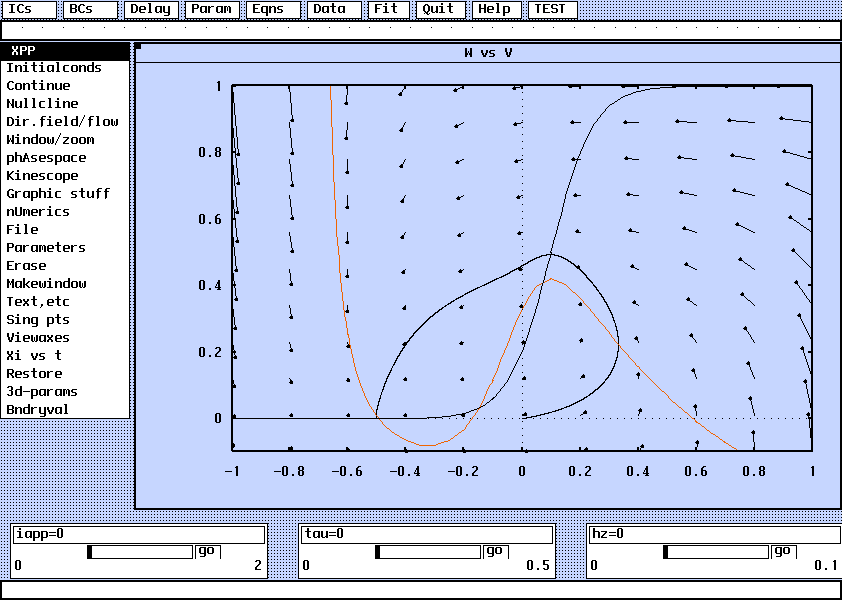
\includegraphics{bitmap/DutchBoy.png}}
\end{tabular}
\normalsize
\end{center}
The actual path of the .xbm image used for a backimage may be different for your installation or OS.



\section{ Examples}

Nothing helps one understand how to use a program better than lots of
examples.  
 
\tc{Morris-Lecar}
\begin{center}
Morris-Lecar Equations
\end{center}
The Morris-Lecar equations arise as a simplification of a model for
barnacle muscle oscillations.  They have the form:
\beqann
C\frac{dV}{dt} &=&
g_L(V_L-V)+g_Kw(V_k-V)+g_{Ca}m_\infty(V)(V_{Ca}-V)+I \\
\frac{dw}{dt} &=& \phi \lambda_w(V)(w_\infty(V)-w)
\eeqann
where
\beqann
m_\infty(V) &=& .5(1+\tanh((V-V_1)/V_2)) \\
w_\infty(V) &=& .5(1+\tanh((V-V_3)/V_4)) \\
\lambda_w &=& \cosh((V-V3)/(2V_4))
\eeqann
This is a very straightforward model and so the equation file is
pretty simple:
\begin{verbatim}
# The Morris-Lecar equations 

# Declare the parameters
p gl=.5,gca=1,gk=2
p vk=-.7,vl=-.5,vca=1
p v1=.01,v2=.145,v3=.1,v4=.15
p i=.2,phi=.333   
  
# Define some functions
minf(v)=.5*(1+tanh((v-v1)/v2))
winf(v)= .5*(1+tanh((v-v3)/v4))
lamw(v)= cosh((v-v3)/(2*v4))

# define the right-hand sides
v'= gl*(vl-v)+gk*w*(vk-v)+gca*minf(v)*(vca-v)+i
w'= phi*lamw(v)*(winf(V)-w)

# some initial conditions -- not necessary but for completeness
v(0)=.05
w(0)=0

# Done!!
d
\end{verbatim}
Note that some errors are now caught by the parser.  For
example, duplicate names and illegal syntax are found.  


Suppose you want to keep track of the calcium current as an auxiliary
variable.  Then, the following file will work
\begin{verbatim}
# The Morris-Lecar equations

# Declare the parameters
p gl=.5,gca=1,gk=2
p vk=-.7,vl=-.5,vca=1
p v1=.01,v2=.145,v3=.1,v4=.15
p i=.2,phi=.333   
  
# Define some functions
minf(v)=.5*(1+tanh((v-v1)/v2))
winf(v)= .5*(1+tanh((v-v3)/v4))
lamw(v)= cosh((v-v3)/(2*v4))

# define the right-hand sides
v'= gl*(vl-v)+gk*w*(vk-v)-gca*minf(v)*(v-vca)+i
w'= phi*lamw(v)*(winf(v)-w)
#
aux ica=gca*minf(v)*(v-vca)

# some initial conditions -- not necessary but for completeness
v(0)=.05
w(0)=0

# Done!!
d
\end{verbatim}
Note that we are wasting computational time
since we compute $I_{Ca}$ twice; once as a contribution to the
potential change and once as an auxiliary variable.  In a FORTRAN or
C program, one would compute it as a local variable and use it in both
instances.  This is the purpose of fixed variables.  (For the present
problem, the computational overhead is trivial, but for coupled arrays
and other things, this can be quite substantial.)  The last program
uses a fixed variable to reduce the computation:
\begin{verbatim}
# The Morris-Lecar equations ml1.ode

# Declare the parameters
p gl=.5,gca=1,gk=2
p vk=-.7,vl=-.5,vca=1
p v1=.01,v2=.145,v3=.1,v4=.15
p i=.2,phi=.333   
  
# Define some functions
minf(v)=.5*(1+tanh((v-v1)/v2))
winf(v)= .5*(1+tanh((v-v3)/v4))
lamw(v)= cosh((v-v3)/(2*v4))

# define the right-hand sides
v'= gl*(vl-v)+gk*w*(vk-v)-icaf+i
w'= phi*lamw(v)*(winf(v)-w)

# where
icaf=gca*minf(v)*(v-vca)

# and
aux ica=icaf

# some initial conditions -- not necessary but for completeness
v(0)=.05
w(0)=0


# Done!!
d
\end{verbatim}
The calcium current is computed once instead of twice.  This is why
``fixed'' variables are useful.


{\bf NOTE:}  Since fixed quantities are not ``visible'' to the user
and auxiliary quantities are not ``visible'' to the internal formula
compiler, we can use the same name for the fixed as the
auxiliary variable; the {\tt aux } declaration essentially makes it
visible to the user with almost no computational overhead. However, it
does generate an error message (not fatal) so it is best to make all
names unique.  
   
\tc{Cable model} \begin{center}
A linear cable equation with boundary conditions
\end{center}
In studying a dendrite, one is often interested in the steady-state
voltage distribution.  Consider a case where the dendrite is held at
$V=V_0$ at $x=0$ and has a leaky boundary condition at $x=1.$
Then the equations are:
\beqann
\lambda^2\frac{d^2V}{dx^2} &=& V(x) \\
V(0)&=& V0 \\
a\frac{dV(1)}{dx} + b V(1) &=& 0
\eeqann
When $a=0,b\ne0$ the voltage at $x=1$ is held at 0.  When $a\ne0,b=0$
there is no leak from the cable and the conditions are for sealed end.
Since this is a second order equation and XPP can only handle first
order, we write it as a system of two first order equations in the
file which is:
\begin{verbatim}
# Linear Cable Model cable.ode

# define the 4 parameters, a,b,v0,lambda^2
p a=1,b=0,v0=1,lam2=1
# now do the right-hand sides
v'=vx
vx'=v/lam2

# The initial data
v(0)=1
vx(0)=0

# and finally, boundary conditions
# First we want V(0)-V0=0
b v-v0
#
# We also want aV(1)+bVX(1)=0
b a*v'+b*vx'
# Note that the primes tell XPP to evaluate at the right endpoint
d
\end{verbatim}
Note that I have initialized $V$ to be 1 which is the appropriate
value to agree with the first boundary condition.  

\tc{Delayed feedback}\begin{center}
The delayed inhibitory feedback net
\end{center}
A simple way to get oscillatory behavior is to introduce delayed
inhibition into a neural network.  The equation is:
\[
\frac{dx(t)}{dt} = -x(t) + f(ax(t)-bx(t-\tau)+P)
\]
where $f(u)=1/(1+\exp(-u))$ and $a,b,\tau$ are nonnegative parameters.
Here $p$ is an input.  The XPP file is:
\begin{verbatim}
# delayed feedback

# declare all the parameters, initializing the delay to 3
p tau=3,b=4.8,a=4,p=-.8
# define the nonlinearity
f(x)=1/(1+exp(-x))
# define the right-hand sides; delaying x by tau
dx/dt = -x + f(a*x-b*delay(x,tau)+p)
x(0)=1
# done
d
\end{verbatim}
Try this example after first going into the numerics menu and changing
the maximal delay from 0 to say, 10.  Glass and Mackey describe a few
other delay systems some of which have extremely complex behavior.
Try them out.



\tc{Random mutation}\begin{center}
A population problem with random mutation
\end{center}
This example illustrates the use of Markov variables and is due to Tom
Kepler.  There are two variables, $x_1,x_2$ and a Markov state
variable, $z.$  The equations are:
\beqann
x_1' &=& x_1(1-x_1-x_2) \\
x_2' &=& z(ax_2(1-x_1-x_2)+\epsilon x_1)
\eeqann
and $z$ switches from 0 to 1 proportionally to $x_1.$  The transition
matrix is 0 everywhere except in the 0 to 1 switch where it is
$\epsilon x_1.$ So z=1 is an absorbing state.

Initial conditions should be $x_1(0)=1.e-4$ or so, $x_2(0)$ the same (this is just
for convenience; we really want $x_2(0)=0$ and then have it jump discontinuously
to $1.e-4$ or so when $z$ makes its transition, but this shouldn't matter that much)


This models the population dynamics of two populations $x_1,x_2$ in competition
with each other.  $x_2$, initially absent, is a mutant of $x_1.$  The mutation rate
$\epsilon$ should be smaller than one.  The relative advantage, $a$,
should be larger than one.

One expects that $x_1$ grows for a while, eventually $z$ makes its transition,
$x_2$ begins to grow and eventually overtakes $x_1.$ 

The equation file for this is
\begin{verbatim}
# Kepler model kepler.ode

init x1=1.e-4,x2=1.e-4,z=0
p eps=.1,a=1
x1' = x1*(1-x1-x2)
x2'= z*(a*x2*(1-x1-x2)+eps*x1)
# the markov variable and its transition matrix
markov z 2
{0} {eps*x1}
{0} {0}
d
\end{verbatim}
\medskip

\tc{Flags and discontinuities}\begin{center}
Some equations with flags
\end{center}
Tyson describes a model which involves cell growth:
\beqann
\frac{du}{dt} &=& k_4(v-u)(a+u^2)-k_6u \\
\frac{dv}{dt} &=& k_1m-k_6u \\
\frac{dm}{dt} &=& bm 
\eeqann

This is a normal looking model with exponential growth of the mass.
However, if $u$ decreases through 0.2, then the ``cell'' divides in
half.  That is the mass is set to half of its value.  Thus, we want to
flag the event $u=.2.$  The file in the {\em new format} (no sense
using the old format since global variables did not appear in earlier
versions of XPP)
\begin{verbatim}
# tyson.ode 
i u=.0075,v=.48,m=1
p k1=.015,k4=200,k6=2,a=.0001,b=.005
u'=  k4*(v-u)*(a+u^2) - k6*u
v'= k1*m - k6*u
m'= b*m
global -1 {u-.2} {m=.5*m} 
d
\end{verbatim}
Everything is fairly straightforward.  When $u-.2$ decreases through
zero tha is, $u$ is greater than .2 and then less than .2, the mass is
cut in half.  Integration using any of the integrators {\em except
ADAMS!} yields a regular limit cycle oscillation.

Another example with discontinuities arises in the study of coupled
oscillators.  Two phase oscillators $x,y$ travel uniformly around the
circle.  If $x$ hits $2\pi$ it is  reset to 0 and adds an amount
$r(y)$ to the phase of $y.$  The XPP file is
\begin{verbatim}
# delta coupled oscillators delta.ode
x'=1
y'=w
global 1 {x-2*pi} {x=0;y=b*r(y)+y}
global 1 {y-2*pi} {y=0;x=b*r(x)+x}
r(x)=sin(x+phi)-sin(phi)
par b=-.25,phi=0,w=1.0
done
\end{verbatim}
Note that there are 2 conditions and each creates 2 events.
\medskip

\tc{Large coupled systems}\begin{center}
Large coupled systems
\end{center}
Many times you want to solve large coupled systems of differential
equations.  Writing the ODE files for these can be a tedious exercise.
The array declaration described above simplifies the creation of ODE
file for this.
For
example, suppose that you want to solve:
\[
\frac{du_j}{dt} = -u_j + f(a\sum_{i=0}^{n-1}\cos\beta(i-j) u_i)
\]
which is a discrete convolution.  Suppose that {\tt n=20} so that this
is 20 equations.  Its not very convenient to type these equations so
instead you can create a simple file in which the equations are typed
just once:
\begin{verbatim}
# chain of 20 neurons
param a=.25,beta=.31415926
u[0..19]'=-u[j]+f(a*sum(0,19)of(cos(beta*([j]-i'))*shift(u0,i')))
f(x)=tanh(x)
done
\end{verbatim}
The {\tt u[0..19]} line with an index spanning {\tt 0} to {\tt 19}
tells XPP to repeat this from 0 to 19.  Thereafter, the string {\tt
[j]} or some simple arithmetic expressions of {\tt j} are evaluated
and substituted verbatim.  
Note how I have used the shift operator on {\tt u0} to make it act like
an array. (Recall that {\tt shift(x,n)} gives the value of the
variable that is defined {\tt n} after the variable {\tt x} is
defined.  

Here is one more example of nearest neighbor coupling in an excitable
medium.  This is a discretization of a PDE.  I will use the analogue
of ``no flux'' boundaries so that the end ODEs will be defined separately.  
\begin{verbatim}
# pulse wave
param a=.1,d=.2,eps=.05,gamma=0,i=0
v0(0)=1
v1(0)=1
f(v)=-v+heav(v-a)
#
v0'=i+f(v0)-w0+d*(v1-v0)
v[1..19]'=i+f(v[j])-w[j]+d*(v[j-1]-2*v[j]+v[j+1])
v20'=i+f(v20)-w20+d*(v19-v20)
#
w[0..20]'=eps*(v[j]-gamma*w[j])
@ meth=modeuler,dt=.1,total=100,xhi=100
done
\end{verbatim}

I only need to define {\tt v0,v20} separately since {\tt w} does not diffuse.
Note how much typing I saved.  




\bigskip











 
  
XPP comes with some other examples that I urge you to look at. A
Volterra example is shown below.

\section{Using xpp}
XPP runs from the command line by typing
\bvb
 xpp <filename>
\end{verbatim}
where {\tt <filename>} is an ODE file as described above.  This argument is optional. 
 If you invoke XPP without the argument, you are asked whether you want to
 read or create a file. Choosing {\tt (r)} to read the file prompts you for an ODE
 file name.  You can get a directory by pressing {\tt <RETURN>}.  If you choose to 
create a new file, you must write a set of commands such as above and then
 save the file.  	It will bounce you out if you make any mistakes. 
 It is not the recommended way to do it -- use an editor and read in the file. 
 XPP will look at the extension of a file and if it is {\tt .dif } the program
 will assume that the model is a difference equation and will treat it as a map. 
 The solution, equilibria, stability and listing of difference equations 
is treated differently from differential equations.  The default plot style 
is also plotting of points instead of lines as for the continuous time case.

\tc{Windows}
\tcc{Main Window}

Once you get a file loaded and it is valid, the program and all of the 
windows will pop up.  There is the main window with the graphics and menus.  
This has several regions on it: the graphics window, the menu window, the command
 window across the top, the message window at the bottom, and three
sliders for binding to parameters.  Initial 
conditions and parameters as well as text labels can be assigned
values in the command window for those who don't like the mouse.  The message 
window gives the position of the pointer and ``tips'' about the
various menu items.  If 
you click the mouse in the main graph and hold it down as you move it, the
coordinates appear in the message window.  The left 
most region is the menu.  Pressing the mouse on a command is the same 
as typing the hot letter for the command and will execute it.  As you
move through the menu items, a brief hint about its maning appears in
the message window. The pointer is 
a hand in the menu window.  {\em In addition to the main window, there
several other windows that will be created.  Due to user demand, these
are all instantly iconified so that you must open them up if you want
to use them.}

\tcc{Initial data,delays,parameters}

In addition to the main window, there is the initial data window which
 contains the names of the variables and the current initial data.  The 
delay window is similar containing the initial data for delay equations. 
 The parameter window contains the list of all parameters and their current
 values.  The boundary condition window is similar with the list of boundary
 conditions given.  These 4 windows constitute the main user editable windows.
  All of the quantities and formulae contained within these can be edited within
 the program.  Clicking on any item in these windows will cause the
 cursor to appear where it can be edited.  If you type the {\tt Enter}
 key after entering the item, the cursor moves to the next item and
 the edited item is accepted.  You can press the {\tt OK} button also
 to accept the item and the pointer is then redirected to the main
 window.  Pressing the {\tt Default} key in the Parameter
 Window will reset the parameters to their values when the program
 boots up.  The {\tt Cancel} button doen't do much of anything yet,
 but maybe someday if I can think of a use! 
 Pressing the {\tt Tab} key is the same as pressing the {\tt Ok} button.
 Pressing {\tt Esc}  exits without changing. 

You can also press the letter {\tt p}  in the main window
to change parameters or simply click
 on the parameter command in the main menu.  Typing {\tt default } will load all 
the parameters with their values when the program first fires up. The
initial data can also be changed from the command window (see below.)  

\tcc{Equation window}

Another window contains the listing of the differential equations. If
 the file is a difference equation, the listing shows this.  These equations 
can be scrolled up and down by pressing the mouse on the {\tt <Up> <Down>} buttons
 or using the cursor keys. Resizing lets you see more and closing iconifies the
 window. Once you are in XPP you cannot alter the differential equations.  Thus
, to solve a different problem you must exit and start again.  I hope to change 
this in the future.  All of these windows can be iconified with no effect on the
 performance of the program.   

\tcc{Browse window}

The other major window contains listings of the numerical values of the solutions 
to the differential equations. 
 This browser window allows you to postprocess
 data and save and load numbers to the disk.
The first few lines contain a variety
of buttons.  The next line has hints about the various buttons that
are given as you move the mouse over the buttons. The names of the
variables, time, and auxilliary variabls are next.  The the numbers
themselves are given. 
  Pressing the cursor keys, the
 {\tt HOME, END, PgUp,PgDn}  keys scrolls you through tthe data either up and down or
 left and right.  Resizing the window lets you see more data.  There are many
 other keys and you can click on the buttons or use the keyboard if the mouse
 pointer is in the Browser.  You can load or save data files by choosing the 
{\tt Load}  and {\tt Save}  keys.  You will be asked for a filename which you should enter.
  Choosing {\tt Get} will load the top row of numbers into the initial data.
 {\tt Find} will find the data row for which the specified variable is closest to
 the specified value.   {\tt Replace} allows you to replace a column by some formula 
involving the column itself and all other columns.  You are asked for the column 
to replace.  Type in one of the names across the top row.  Then you are asked 
for the formula.  Type it in and the entire column will be replaced.  For example 
if the names of your variables are {\tt X}  and { \tt Y}  and you
choose {\tt X } as the column
 to replace and type 
\bvb 
       X^2 + T*Y
\end{verbatim}
then the column {\tt X } will be replaced by the function at each row.  If the first 
character in the formula is the {\tt \& } symbol, an integral of the formula will be
 placed in the specified column.  If the formula is anything of the form :
\bvb
	@<variable>
\end{verbatim}
the numerical derivative of the {\tt <variable> } will be computed ad placed in the
 column. 
If the formula has the form:
\bvb
 lo:hi
\end{verbatim}
the the column will be replaced by an arithmetic series starting at
{\tt lo} and ending at {\tt hi}.
If the formula has the form:
\bvb
 lo;inc
\end{verbatim}
the the column will be replaced by an arithmetic series starting at
{\tt lo} incrementing by {\tt inc.} 

Choosing {\tt Unreplace} will restore the most recent column.  Each time you integrate
 the equations or solve a boundary value problem or look at a range of equilibria, 
the numbers are replaced by the most recent.  You must save the data to a
 file to use it again.  Pressing {\tt First}  and {\tt last} will mark the data so that you 
can save a portion or restore a portion.  {\tt Home} takes you to the beginning and
 {\tt End} to the end of the list. 

The {\tt Table} key allows you to save a column as a ``table'' file
which can be used in XPP as a function.  

\tcc{Parameter sliders}  These are really cool and I stole the idea
from Madonna, a Mac ODE solver. Click on one of them where it says
{\tt Parameter} and fill it in.  These bind the slider to a particular
parameter.  You set the low and high values of the slider and the
current value.  Click {\tt OK} to accept. Change them by clicking on
the name window.  Then move the mouse to the slider and pressing it,
move it around.  When done, you have set the parameter to the
indicated value.


Other windows are opened on occasion and can remain open throughout the
 session.  The usual methods for resizing windows works on the graphics and
 listing and browser windows.

When there are multiple graphics windows, only one is active at a given time
 and only one can be drawn to.  The window is made active by clicking the
 left button when inside the window.  A little square appears in the upper left
 corner of the window to indicate its activity.  The variables on the
 axes are given in the title of the window and are Z-Axis vs Y-Axis vs X-Axis.  


Two other windows appear permanently, when needed: the Equilibrium window
 that gives values and stability of the most recently computed
 equilibrium and the AUTO window for bifurcation analysis.


The main commands are on the first menu and the numerics menu.  Communication 
to the program is via the keyboard and the mouse and through parameter boxes
 that are displayed.  Almost all commands have keyboard shortcuts so that if
 you know the original DOS version, you can use the X version with little help.  
When you are prompted for floating point numbers at the command line, then 
you can insert either numbers or mathematical expressions provided the first
 character is the {\tt \%} symbol. Thus if you want to input {\tt sin(1.5)} as a floating 
point number, you would write
\bvb
          %sin(1.5)
\end{verbatim}
at the command line. You can enter such expressions in the parameter and
initial data windows and these are converted to numbers.  
 

\section{The main commands}
All commands can be invoked by typing the hot key for that command (capitalized
 on the menu) or clicking on the menu with the mouse.  Usually most commands can
 be aborted by pressing the {\tt Esc} key. Once one of these is chosen, the
 program begins to calculate and draw the trajectories.  If you want to
 stop prematurely, press the {\tt Esc} key and the integration will
stop. 

\begin{description}

\tc{ICs}\item[(I)nitial conds] This invokes a list of options for integrating the
 differential equations.  The choices are:
\begin{description}
\item[(R)ange]  This lets you integrate multiple times with the results shown
 in the graphics window.  Pressing this option produces a new window with
 several boxes to fill in.  First choose the quantity you want to range
 over.  It can be a parameter or a variable.  The integrator will be called
 and this quantity will be changed at the beginning of each integration.
  Then choose the starting and ending value and the number of steps. The
 option Reset storage only stores the last integration.  If you choose not
 to reset, each integration is appended to storage.  Most likely, storage
 will be exceeded and the integration will overwrite or stop. The option 
to use last initial conditions will automatically use the final result of
 the previous integration as initial dat for the next integration.  Otherwise,
 the current ICs will be used at each step (except of course for the  variable
 through which you are ranging.) 
If you choose {\tt Yes} in the {\tt Movie} item,
then after each integration, XPP will take a snapshot of the picture.
You can then replay this series of snapshots back using the Kinescope.
When you are happy with the parameters, simply
 press the OK button.  Otherwise, press the Cancel button to abort.  Assuming
 that you have accepted, the program will compute the trajectories and plot 
them storing none of them or all of them.  If you press {\tt Esc} it will abort the 
current trajectory and move on to the next.  Pressing the {\tt / } key will abort
 the whole process. 
\item{(2)par range} is similar to range integration but allows you to
range over two items. The {\tt Crv(1) Array(2)} item determines how
the range is done. If you choose {\tt Crv} then the two paramaters are
varied in concert, $[a(i),b(i)]$ for $i=0,\ldots,N$. The more useful
{\tt Array} varies them independently as $[a(i),b(j)]$ for
$i=0,\ldots,N$ and $j=0,\ldots,M.$    
\item[(L)ast]  This uses the end result of the most recent integration as the
 starting point of the curret integration.
\item[(O)ld] This uses the most recent initial data as the current initial 
data.  It is essentially the same as Go.
\item[(G)o] which uses the initial data in the IC window and the current
 numerics parameters to solve the equation.  The output is drawn in the
 current selected graphics window and the data are saved for later use.  The
 solution continues until either the user aborts by pressing {\tt Esc}, the
 integration is complete, or storage runs out.
\item[(M)ouse]  allows you to specify the values with the mouse.  Click at the
 desired spot.
\item[(S)hift] This is like Last except that the stating time is shifted to the 
current integration time.  This is irrelevant for autonomous systems but is
 useful for nonautonomous ODEs.
\item[(N)ew] This prompts you at the command line for each initial condition.
 Press {\tt Return} to accept the value presented.
\item[s(H)oot] allows you to use initial data that was produced when
you last searched for an equilibrium.  When a rest state has a single
positive or negative eigenvalue, then XPP will ask if you want to
approximate the invariant manifold.  If you choose {\tt yes} to this,
then the initial data that were used to compute the trajectories are
remembered.  Thus, when you choose this option, you will be asked for
a number 1-4.  This number is the order in which the invariant
trajectories were computed.  Note if the invariant set is a stable
manifold, then you should integrate backwards in time.
\item[(F)ile] prompts you for a file name which has the initial data
as a sequence of numerical values.
\item[form(U)la] allows you to set all the initial data as a
formula. This is good for systems that represent chains of many ODEs.
When prompted for the variable, type in {\tt u[2..10]} for example to
set the variables {\tt u2,u3, ..., u10} and then put in a formula
using the index {\tt [j]}. Note you must use {\tt [j]} and not {\tt j}
by itself. For example {\tt sin([j]*2*pi/10)}. Repeat this for
different variables hitting enter twice to begin the integration.
\item[M(I)ce] allows you to choose multiple points with the
mouse. Click Esc when done.
\item[(D)AE guess] lets you choose a guess for the algebraic variables of
the DAE.
\item[(B)ackward] is the same as ``Go'' but the integration is run
backwards in time.
  
\end{description}
\tc{Continue}\item[(C)ontinue]  This allows you to continue integrating appending the data
 to the 
current curve. Type in the new ending time.
\tc{Nullclines}\item[(N)ullclines]  This option allows you to draw the nullclines of systems.  
They are most useful for two-dimensional models, but XPP lets you draw them for
 any model.  The constraints are the same as in the direction fields option
 above.  The menu has 4 items.
\begin{description}
\item[(N)ew] draws a new set of nullclines.
\item[(R)estore] restores the most recently computed set.
\item[(A)uto] turns on a flag that makes 
XPP redraw them every time it is necessary because some other window obscured
 them.
\item[(M)anual] turns this flag off so that you must restore them manually.
 The X-axis nullcline is blue and the Y-axis nullcline is red.
\item[(F)reeze] allows you to freeze and play back multiple nullclines
\begin{description}
	\item[(F)reeze] freezes the current nullclines
	\item[(D)elete all] deletes all frozen nullclines
	\item[(R)ange] lets you vary a parameter through some range,
	computes the nullclines and stores them
	\item[(A)nimate] redraws all the frozen nullclines erasing the
screen between each one. The user specifies a delay between drawing.
\end{description}
\item[(S)ave] saves the nullclines into a file. They can then be
plotted using other software. {\bf NOTE:} The way that XPP computes
nullclines (by computing zero contours of a two-variable function)
means that the nullclines are composed of a series of small line
segments. This means that if you try to plot them as a continuous
curve, your plotting program will produce garbage. Thus, you should
plot them as points and not draw line segments between them. The data
file produced has 4 columns. The first two are the ``x'' nullcline and
the second two are the ``y'' nullcline. Data is as follows:
\begin{verbatim}
xnx1 xny1 ynx1 yny1
xnx2 xny2 ynx2 yny2
...
\end{verbatim}
There are an even number of entries. The ``x'' nullcline consists of
segments {\tt (xnx1,xny1),(xnx2,xny2)} between pairs of
points. Similarly for the ``y'' nullcline.
 
\end{description}
\tc{Direction Field/Flow}\item[(D)irection Field/Flow]
This option is best used for two-dimensional systems however,
 it can be applied to any system.  The current graphics view must be a
 two-d plot in which both variables are different and neither is the time
 variable, T.  There are five items.
\begin{description}
\item[(D)irection fields] Choosing the direction field option will prompt you for 
a grid size.  The two dimensional plane is broken into a grid of the size
 specified and lines are drawn at each point specifying the direction of 
the flow at that point. The length of the line gives the 
magnitude. If the system is more than two-dimensional, the
 other variables will be held at the values in the initial conditions
window.
\item[(F)low] Choosing the flow, you will be prompted for a grid size
and
 trajectories
 started at each point on the grid will be integrated according to the
 numerical parameters.  Any given trajectory can be aborted by pressing 
{\tt Esc} and the whole process stopped by pressing {\tt /}.  The
remaining
 variables 
if in more than two-dimensions are initialized with the values in the
IC window. 
\item[(N)o Dir Field] turns off redrawing of direction fields when you
click on (Redraw).  Erasing the screen automatically turns this off.
\item[(C)olorize] This draws a grid of filled rectangles on the screen
whose color is coded by the velocity or some other quantity. (See the
Numerics Colorize menu item).
\item[(S)caled Dir. Fld] is the same as (D)irection field but the
lengths are all scaled to 1 so only directional information is given.
\end{description}


\tc{Window}\item[(W)indow] allows you to rewindow the current graph.  Pressing this presents 
another menu with the choices:
\begin{description}
	\item[(W)indow]  A parameter box pops up prompting you for the values.  
Press OK or CANCEL when done.
	\item[(Z)oom in]  Use the mouse to expand a region by clicking, dragging and 
releasing.  The view in the rectangle will be expanded to the whole window.
	\item[Zoom (O)ut]  As above but the whole window will be shrunk into the 
rectangle.
	\item[(F)it]  The most common command will automatically fit the window so 
the entire curve is contained within it.  For three-D stuff the window data 
will be scaled to fit into a cube and the cube scaled to fit in the window. 
Use this often.
\end{description}
(NOTE:  On some displays, no rubber boxes are drawn for the zooming
operations.  If this occurs, start XPP with the {\tt -xorfix} command
line flag.)
\tc{Phase Space}\item[ph(A)se space]  XPP allows for periodic domains so that you can solve 
equations on a torus or cylinder.  You will be prompted to make (A)ll variables
periodic, (N)o variables periodic or (C)hoose the ones you want.  You will 
be asked for the period which is the same for all periodic variables (if they 
must be different, rescale them) Choose them by clicking the 
appropriate names from the list presented to you. An {\tt X} will
appear next to the selected ones.  Clicking toggles the {\tt X}. 
 Type {\tt Esc} when done or CANCEL or DONE.
 XPP mods your variables by this period and is smart
 enough when plotting to not join the two ends. 

\tc{Kinescope}\item[(K)inescope]  This allows you to capture the bitmap of the active window and
 play it back.  
Another menu pops up with the choices:
\begin{description}
\item[(C)apture] which takes a snapshot of the 
currently active window
\item[(R)eset] which deletes all the snapshots
\item[(P)layback] which cycles thru the pictures each time you click the left mouse 
button and stops if you click the middle. 
\item[(A)utoplay] 
continuously plays back snapshots. You tell it how many cycles
and how much time between frames in milliseconds.
\item[(S)ave] Save the frames in either ppm or gif format
\item[(M)ake anigif] Create an animated gif from the frames. The
file is always called {\tt anim.gif} and can be played with Netscape, Explorer,
xanim, etc.
\end{description}


\tc{Graphics}\item[(G)raphic stuff]  This induces a popup menu with several
choices.
\begin{description}
\item[(A)dd curve]  This lets you add another curve to the picture. A 
parameter box will appear aking you for the variables on each axis, a color,
 and line type (1 is solid, 0 is a point, and negative integers are
small circles of increasing radii.) All 
subsequent integrations and restorations will include the new graph.  Up to 
10 per window are allowed.
\item[(D)elete last]  Will remove most recent curve from the added list.
\item[(R)emove all] Deletes all curves but the first.
\item[(E)dit curve]  You will be asked for th curve to edit.  The first is 0,
 the second 1, etc.  You will get a parameter box like the add curve
option.
\item[(P)ostscript]  This will ask you for a file name and write a postscript
 representation of the current window.  Nullclines, text, and all
graphs will be 
 plotted.  You will be asked for Black and White or Color.  Color tries
to match the color on the screen.
Black and white will use a variety of dashed curves
for the plots. The Land/Port option lets you draw either in
Landscape (default) or Portrait style.  Note that Portrait is rather
distorted and is created in for those who cannot rotate their
postscript plots. Font size sets the size of the fonts on the
axes.   
\item[(F)reeze]  This will create a permanent curve in the window.  Usually, 
when you reintegrate the equations or load in some new data, the current curve 
will be replace by the new data.  Freeze prevents this.  Up to 26 curves can be
 frozen.  
\begin{description}
\tc{Freezing Curves}
\item[(F)reeze ] This freezes the current curve 0 for the current
plotting window.  It will not be plotted in other windows. If you
change the axes from 2 to 3 dimensions and it was frozen as a 2D curve
(and {\em vice versa} ) then it will also not be plotted. It is better
to create another window to work in 3 dimensions so this is avoided.
 A parameter box
pops up that asks you for the color (linetype) as well as the key name
and the curve name.  The curve name is for easy reference and should
be a few characters.  The key name is what will be printed on the
graph if a key is present.
\item[(D)elete]  This gives you a choice of available curves to
delete.
\item[(E)dit] This lets you edit a named curve; the key, name, and
linetype can be altered.   
\item[(R)emove all]  This gets rid of all of the frozen curves in the
current window.
\item[(K)ey] This turns the key on or off.  If you turn it on, then
you can position it with the mouse on the graph.  The key consists of
a line followed by some text describing the line.  Only about 15
characters are permitted.
\item[(B)if.diag] will prompt you for a filename and then using the
current view, draw the diagram. The file must be of the same format as
is produced by the {\tt Write pts} option in the AUTO menus. (see AUTO
below.)  The diagram is colored according to whether the points are
stable/unstable fixed points or periodics. The diagram is ``frozen''
and there can only be one diagram at a time.  
\item[(C)lr. BD] clears out the current bifurcation diagram.
\item[(O)n freeze] Toggles a flag that automatically freezes the
curves as you integrate them.
\end{description}
\item[a(X)es opts]  This puts up a window which allows you to tell XPP
where you want the axes to be drawn, whether you want them, and what
fontsize to make the PostScript axes labels.  
\item[exp(O)rt]  This lets you save the points that are currently
plotted on the screen in XY format. Thus if you have a phaseplane on
the screen, only the X and Y values are saved. This makes it
compatible with porgrams like XMGR which assume X Y1 Y2 ... data. If
you have several traces on the screen at once, it saves the X values
of the first trace and the Y values of the first and all subsequent
traces.
\item[(C)olormap] This lets you choose a different color map from the
default. There are a bunch of them; try them all and pick your
favorite. 

\end{description}

\item[n(U)merics] This is so important that a section is devoted to
it. See below.

\tc{File}\item[(F)ile] 
This brings up a menu with several options. Type {\tt Esc} to abort.
\begin{description}
\item[(P)rt info] Brings up a window with the source code for
the ODE file. If you click on {\tt Action} it brings up the active
comments so you can make little tutorials.
\item[(W)rite set] This creates a file with all of the info about the
current numerics, etc as well as all of the currently highlighted
graphics window.  It is readable by the user. It in
some sense saves the current state of XPP and can be read in later.
\item[(R)ead set]  This reads a set that you have previously written.
 The files are very tightly connected
 to the current ODE file so you should not load a saved file from one equation 
for a different problem.
\item[(A)uto] This brings up the AUTO window if you have installed
AUTO. See below for a description of this.
\item[(C)alculator] This pops up a little window.  Type formulae in
the command 
line involving your variables and the results are displayed in the popup.  Click
 on Quit or type {\tt Esc} to exit.
\tc{Edit right-hand sides} \item[(E)dit]  You can edit the equations from within
XPP.  {\em Note that XPP is capable of understanding right-hand sides of up
to 256 characters.  However, the RHS editor will not accept anything
longer than about 72 characters.}  This menu item presents a
list of four options:
\begin{description}
\item[(R)HS] Edit the right-hand sides of the ODEs IDEs, and auxiliary
variables. If you are happy with the editing, then type {\tt TAB} or
click on {\tt OK.}  The program will parse the new equations and if
they are syntactically correct, alter the corresponding equation.  If
there is an error, the you will be told of the offending
right-hand-side and that will not be changed.  
\item[(F)unctions] This lets you alter any user-defined functions.  It
is otherwise the same as the above.
\item[(S)ave as] This creates an ``ODE'' file based on the current
parameter values, functions, and right-hand sides.  You will be asked
for a filename.
\item[(L)oad DLL] invokes the dynamic linker. You can load in
complicated RHS's that would be awkward to create using XPP's simple
language. 
\end{description}
\item[(S)ave info] This is like {\tt (P)rt info} but saves the info to
a file.  It is human readable.
\item[(B)ell on/off]  This toggles the stupid noisy bell on and off.
\item[C-(H)ints] spews out stuff to the terminal that represents a
skeletal C program for the right-hand sides.  Presumably, you could
use this to create faster code by replacing the file {\tt myrhs.c}
with your compiled version. Hah! I don't khow why this is even here --
Good luck!. 
\item[(Q)uit]  This exits XPP first asking if you are sure.
\item[ (T)ranspose ]  This is not a very good place to put this but I
stuck it here just to get it into the program.  The point of this
routine is to allow one to transpose chunks of the output.  For
example, if you are solving the discretization of some spatial problem
and find a steady state, there is no way to plot the steady state as a
function of the index of the discrete system.  This routine lets you
do that.  The idea is to take something that looks like:
\begin{verbatim}
t1  x11  x21  x31 ... xm1 
t2  x12  x22  x32 ... xm2
...
tn  x1n  x2n  x3n ... xmn
\end{verbatim}
and transpose some subset of it. You are prompted for 6 items.  They
are the name of the first column you want to index, the number of
columns ({\tt ncols} and amount you want to skip across columns, {\tt
colskip} (so that {\tt colskip = 2} would be every other column.  You
must also provide the starting row {\tt j1}, the number of rows, {\tt
nrows} and the row skip, {\tt rowskip.} the The storage array is temporarily
replaced by a new array that has {\tt M=ncols} rows and {\tt nrows+1}
columns (since the data is transposed, the rows and columns are as
well; confusing ain't it).  The form of the array is:
\begin{verbatim}
1  x(i1,j1) x(i1,j2) x(i1,j3) ...
2  x(i2,j1) x(i2,j2) x(i2,j3) ...
...
M  x(iM,j1) x(iM,j2) x(iM,j3) ...
\end{verbatim}
where {\tt i2=i1+colskip, i3=i1+2*colskip, ...} and {\tt i1} is the
index corresponding to the name of the first column you
provide. Similarly, {\tt j2=j1+rowskip, ...}. As a brief example,
suppose that you solve a system of equations of the form:
\[
 x_j' = f(x_{j-1},x_j,x_{j+1},I_j)
\]
where $j=1,\dots,20.$ Click on transpose and choose {\tt x1} as the
first column, {\tt colskip=1, ncols=20} and say {\tt row1=350,
nrows=1,rowskip=1} then a new array will be produced. The first column
is the index from 1 to 20 and the second is {\tt xj(350)} where 350 is
the index and not the actual value of time. By plotting the second
column versus the first you get a ``spatial profile.'' 
\item[t(I)ps] This toggles the tips on and off that appear in the
message line.
\item[(G)et par set] This loads one of the parameter sets that you
have defined in the ODE file.

\end{description}
\tc{Parameters}\item[(P)arameters]    Type the name
 of a parameter to change and enter its value. Repeat for more
 parameters.  Hit {\tt Enter} a few times to exit.   Type 
{\tt default} to get back the values when you started XPP. Use this if
 you don't want to mess with the mouse.
\tc{Erase}\item[(E)rase] erases the contents of the active window, redraws the
axes, 
deletes all 
text in the window, and sets the redraw flag to Manual.
\tc{Multiple windows}\item[(M)ake window]   The option allows
 you to create and destroy graphics windows. There are several
choices.
\begin{description}  
\item[(C)reate] makes a copy of the currently active window and makes itself active.
  You can change the graphs in this window without affecting the other windows. 

\item[(K)ill all]  Removes all but the main graphics window.

\item[(D)estroy]  This destroys the currently active window.  The main window
 cannot be destroyed.  
\item[(B)ottom] puts the active window on the bottom. 
\item[(A)uto] turns on a flag so that the window will automatically be
redrawn when needed.

\item[(M)anual] turns off the flag and the user must restore the picture manually.
\item[(S)imPlot on/off] lets you plot the solution in all active
windows while the simulation is running. This slows you down quite a
bit.  

\end{description}
After a window is created, you can use the mouse to find the
coordinates by pressing and moving in the window.  The coordinates are
given near the top of the window.
\tc{Adding text etc}\item[(T)ext, etc] allows you to write text to the
display in a variety of sizes and in two different fonts.  You can
also add other symbols to your graph. 
\begin{description}
\item[Text] This prompts you for the text you want to add.  Then you
are asked for the size; there are five choices (0-5): 0-8pt, 1-12pt, 2-14pt,
3-18pt, 4-24pt. Text also has several escape sequences:
\begin{itemize}
\item $\backslash$1 -- switches to Greek font 
\item $\backslash$0 -- switches to Roman font 
\item $\backslash$s -- subscript
\item $\backslash$S -- superscript
\item  $\backslash$n -- neither sub nor superscript
\item $\backslash$\{expr\} -- evaluate the expression in the braces before 
  rendering.
\end{itemize}

Note that not all X-servers will have these fonts, but the
postscript file will still draw them. Finally, place the text with the
mouse.
\item[Arrow] This lets you draw an arrow-head to indicate a direction
on a trajectory.  You will be prompted for the size, which should be
some positive number, usually less than 1.  Then you must move the the
mouse and select a direction and starting point.  Click on the
starting point and holding the mouse button down, drag the mouse to
indicate the direction of the arrow-head. Then release the
mouse-button and the arrow will be drawn.  
\item[Pointer] This is like an arrow, but draws the stem as well as
the arrow head.  It can be used to point to important features of your
graph. The prompts are like those for {\tt Arrow.}
\item[Marker] This lets you draw little markers, such as triangles,
squares, etc on the picture. When prompted to position the marker with
the mouse, you can over-ride the mouse and manually type in
coordinates if you hit the (Tab) key.
\item[Edit] This lets you edit the text, arrows, and pointers in one of
three ways:
\begin{description}
\item[Move] lets you move the object to another location without
changing any of its properties.  Choose the object with the mouse by
clicking near it.
You will then be prompted as to whether you want to move the item that
XPP selected.  If you answer {\tt yes} use the mouse to reposition it.
\item[Change] lets you change the properties: for text, the text
itself, size, and font can be change; for arrows and pointers, only
the size of the arrow head can be changed. As above, select the object
with the mouse and then edit the properties.
\item[Delete] deletes the object that you select with the mouse.
\end{description}
\item[(D)elete All] Deletes all the objects in the current window.
\item[marker(S)] This is similar to the Marker command, but allows you to
automatically mark a number of points along a computed trajectory. You
use the data browser to move the desired starting point of the list to
the top line of the browser. Then click on the (Text) (markerS)
command and choose a size and color. Then tell XPP how many markers
and how many browser lines to jump between markers. (Thus, 10 would
put a marker at every 10th data point).. 



\end{description}


\tc{Equilibria}\item[(S)ing pts]  This allows you to calculate
equilibria for a discrete or continuous system.  The program also
attempts to determine stability for delay-differential equations (see
below in the numerics section.) There
 are three options.
\begin{description} 
	\item[(G)o] begins the calculation   using the values in the initial 
data box as a first guess.  Newton's method is applied.  If a value is found XPP
 tries to find the eigenvalues and asks you if you want them printed out.  If so,
 they are written to the console.  Then if there is a single real positive or
 real negative eigenvalue, the program asks you if you want the unstable or
 stable manifolds to be plotted.  Answer yes if so and they will be
 approximated. The calculation will continue until either a variable
goes out
 of bounds or you press {\tt Esc}.  If {\tt Esc} is pressed, the other
branch is
 computed. (Unstable manifolds are yellow and computed first followed
by the stable manifolds in color turquoise.) 
 The program continues to find any other invariant sets until it has gotten 
them all.  These are not stored, however, the initial data needed to
create them are and can be accessed with the {\tt Initial Conds} {\tt
sHoot} command. 
Once an 
equilibrium is computed a window 
appears with info on the value of the point and its stability.  The top of 
the window tells you the number of complex eigenvalues with positive,{\tt (c+)}, 
negative {\tt (c-)}, zero {\tt (im)}  real parts and the number of
real positive
{\tt  (r+)}  and 
real negative { \tt (r-)}  eigenvalues. If the equation is a difference equation, 
then the symbols correspond the numbers of real or complex eigenvalues 
outside {\tt (+)}  the unit circle or inside { \tt (-)}
This window remains and can be iconified. 
\item[(M)ouse]  This is as above but you can specify the initial guess by 
clicking the mouse.  Only the two variables in the two-D window will reflect 
the mouse values.  This is most useful for 2D systems.
\item[(R)ange]  This allows you to find a set of equilibria over a range
 of parameters.  A parameter box will prompt you for the parameter, starting
 and ending values, number of steps.  Additionally, two other items are 
requested.  Column for stability will record the stability of the equilibrium 
point in the specified column (Use column number greater than 1).  
If you elect to shoot at each, the invariant 
manifolds will be drawn for each equilibrium computed.  The stability can be 
read as a decimal number of the form {\tt  u.s } where {\tt s}  is the
number of stable and {\tt u} 
 the number of unstable eigenvalues. So {\tt 2.03} means 3 eigenvalues
with negative real parts (or in the unit circle) and 2 with positive
real parts (outside the unit circle.)  
For delay equations, if a root is found, its real part is included in
this column rather than the stability summary since there are
infinitely many possible eigenvalues.
The result of a range calculation is saved 
in the data array and replaces what ever was there.  The value of the parameter
 is in the time column, the equilibria in the remaining columns and the 
stability info in whatever column you have specified. 
 {\tt Esc} aborts one step and 
{\tt /}  aborts the whole procedure. As with the initial data/range
option, you can also make a movie.  This is useful mainly for systems
where invariant sets are to be computed.
\end{description} 
\tc{Axes}\item[(V)iew axes]  This selects one of  different types of graphs: 
a 2D box or a 3D Box; brings up a threed window; or lets you create
animations of your simulation. 
If you select the 2D curve, you will be asked for limits 
as in the window command as well as the variables to place on the axes
and the labels for the axes.   
3D is more complicated.  You will be asked for the 3 variables for the 3 axes, 
their max and min values and 4 more numbers, {\tt XLO},  etc.  XPP first scales the 
data to fit into a cube with corners (-1,-1,-1) and (1,1,1).  Rotation of this
 cube is performed and then projected into the two-D window.  {\tt XLO}, etc define
 the scales of this projection and are thus unrelated to the values of your 
data.  You are also asked for labels of the axes.
Use the {\tt (F)it } option if you don't know whats going on.
\tc{Space-time plots} (A)rray plots introduce a new window that lets the user plot many
variables at once as a function of time with color coded values.  The
point is to let one plot, e.g., an array of voltages, {\tt V1, V2,
..., VN} across the horizontal as time varies in the vertical
dimension. For example, suppose you have discretized some PDE and want
to see the evolution in space and time of the variables.  Then use
this plotting option. You will be prompted for the first column name
of the ``array'', then number of columns, the first row, then number
of rows, and the number of rows to skip. For example, if the
discretized PDE variables are {\tt u0,u1, ... ,u50}, then type in {\tt
u0} for the first element and {\tt 51} for the number of columns.
If you want rows 200
through 800 only every 4th time unit, you would put 200 for the first
row, 201 as the number of rows, and 4 as the skip value.  
You can also set the column skip as well. This is useful if you have
defined a series of variables with the array blocks. If the array
block is for a two-component system, then plot every 2, so you would
put 2 in this entry. The {\tt Print}
button asks you for a file name and  top and bottom labels and a
render style. The render styles are:
\begin{description}
\item{-1} Grey scale
\item{0} Blue-red
\item{1} Red-Yellow-Green-Blue-Violet
\item{2} Like 1 but periodic
\end{description}
The {\tt Style} button does nothing yet. The {\tt Edit} button lets
you change ranges and arrays to plot. The {\tt Redraw} button is obvious.

Since the animation option requires learning
lots of new stuff, see section \ref{toon} for a description of the
animation language and what you can do with it.

\tc{Time plots}\item[(X)i vs t]  This chooses a certain 2D view and prompts you for the variable name. 
 The window is automatically fitted and the data plotted.  It is a
shortcut to choosing a view and windowing it.
\tc{Redrawing}\item[(R)estore] redraws the most recent data in the browser in accordance with the
 graphics parameters of the active window.
\tc{3D Parameters}\item[(3)d params]  This lets you choose rotations of the axes and
perspective  planes. 
 Play with this to see. You must be have a 3D view in the active graph
to use this. 

\tcc{3D movies!} There is another selection: {\tt Movie}.  If you choose {\tt
Yes} for this, then after you click {\tt Ok}, you will be prompted for
some additional parameters.  There are two angles you can vary, {\tt
theta} and {\tt phi}. Choose one, give an initial value, an increment,
and the number of rotations you want to perform.  XPP will then use
the {\tt Kinescope} to take successive snapshots of the screen after
performing each rotation.  You can then play these back from the
Kinescope or save them as an animated gif. 
  
\tc{Boundary values}\item[(B)ndry val]  This solves boundary value problems by numerical shooting. There
 are 4 choices.
\begin{description}
\item[(S)how]  This shows the successive results of the shooting and 
erases the screen at the end and redraws the last solution.  The program
 uses the currently selected numerical integration method, the current starting
 point, {\tt T0} as the left end time and  {\tt T0+TEND} as the right
end. 
 Thus, if the
 interval of interest is {\tt (2.5,6)} then set {\tt T0=2.5} and {\tt
TEND=3.5} in the numerics menu.  
\item[(N)o show] This is as above but will not show successive solutions.
\item[(R)ange]  This allows you to range over a parameter keeping starting or
 ending values of each of the variables.  A window will appear asking you for
 the parameter, the start, end, and steps.  You will also be asked if you want 
to cycle color which means that the results of each successful solution to the
 BVP will appear in different colors. Finally the box labeled{\tt  side} tells the
 program whether to save the initial {\tt (0)} or final{\tt (1)}
values of 
the solution. 
 As the program progresses, you will see the current parameter in the info
 window under the main screen.  You can abort the current step by
pressing
 {\tt Esc} 
and the whole process by pressing {\tt /}. As in the {\tt Initialconds
Range} option, you can also choose {\tt Movie}.  Then, as before,
after each solution is computed, a snapshot is take.  Thus, you can
playback the solutions as a function of the range parameter.

\item[(P)eriodic] Periodic boundary conditions can be solved thru the
usual methods, but one then must write an addition equation for the
frequency parameter.  This option eliminates that need so that a 2-D
autonomous system need not be suspended into a 3D one.  You will be
asked for the name of the adjustable parameter for frequency.  You
will also be asked for the section variable and section.  This is an additional
condition that must be satisfied, namely, $x(0)=x_0$ where $x$ is the
section variable and $x_0$ is the section.  Type {\tt yes} if you want
the progress shown.  
\end{description}
\end{description}


\section{Numerical parameters}
When you click on the {\tt nUmerics} command in the main menu, a new
list appears.  This is the numerics menu and allows you to set all of
the numerical parameters as well as some post-processing.  Some of
these may not yet be implemented. Press {\tt Esc} or click on the {\tt
exit} to get the main menu back.

The items on this menu are:
\begin{description}
\tc{Time control}\item[(T)otal] This is the amount of time to integrate. It is called
{\tt TEND} in the documentation.  If it is
negative 
then it will be 
made positive and no data will be stored. Thus you can integrate for very long 
periods of time without being told that the storage is full.
\item[(S)tart time] This is the initial time {\tt T0} For autonomous
systems it is usually irrelevant. 
\item[tRansient] The program will integrate silently for this amount
of time before plotting output.  It is used to get rid of transients.
\item[(D)t] This is the step size used by the fixed step integrators
and the
 output step
 for Gear,CVODE, Quality RK, Rosen,and Stiff algorithms.  
It is positive or negative depending on the
direction of integration.    
 \tc{Iteration control} \item[n(C)line ctrl] will prompt you for the grid size for computing
nullclines. 
\item[s(I)ng pt ctrl]  This prompts you for errors and epsilons for eigenvalues 
and equilibria calculations as well as the maximum iterates.  If you
have global flags, then you will be asked for {\tt smin} as well.

\item[n(O)ut]  This sets the number of integration steps to perform
between output 
to
 storage.  Thus, if you output every 10 steps with a {\tt Dt} of .05, XPP will yield
 output at times that are $10*.05=.5$ timesteps apart.  The advantage of this 
is that lengthier records of data can be made without losing accuracy of the 
integrator.  This parameter is also used in the continuation of fixed
point for maps in AUTO. If this parameter is $n>1$, then in
AUTO, the fixed point of  $F^(n)(x)$ is found where $F$ is the
right-hand side of the equations. This allows AUTO to continue
periodic points of maps.

\item[(B)ounds]  This sets a global bound on the integrator.  If any variable exceeds
 this value in magnitude, a message appears and the integration stops.
\tc{Numerical method}\item[(M)ethod]  allows you to choose the methods of integration.
DoPri5, DoPri83, Gear, CVODE, Quality RK, Rosen,and Stiff  are
 adaptive. The first two are the Dormand-Prince integrators and are
the most modern of the group.
 Gear,CVODE, Rosen, and Stiff are the best to use for stiff problems.  If you choose
the adaptive methods, you will be
 asked for error tolerance, minimum step, and maximum step size.  The discrete
 method should be used for difference equations.  
If you choose CVODE/Rosen, you can choose to use the banded version of
it. You should set the upper and lower bandwidths. Note that this is
recommended for stiff PDEs only and should be used in conjunction with
the block arrays.  
You can get huge speed up in the integration. I have gotten 100
fold on some problems. If the method is
adaptive, the
 output {\tt NOUT} is set to 1.  Also the adaptive methods generate several possible error messages
 that you may have to respond to.  These suggest how to fix the error.
 Markov processes are ignored by GEAR.
 Backward Euler prompts you for a tolerance and the maximum number of iterates
 for each step. The Volterra method, described below, prompts for
a tolerance, maximum iterates, and a ``memory size.''   You will also
be asked if you want the convolution kernels to be re-evaluated after
any parameter is changed in either the range integration or through a
manual change in parameters.  If this flag is 1 then the kernels will
be re-computed.  The default is to not recompute them. Memory size
determines how far back to save the results for the integrator. If
this is small, there is a big speed-up in the integration, but you
could be neglecting important terms.  The symplectic integrator should
only be used for systems of the form:
\begin{eqnarray*}
x_1' &=& v_1 \\
v_1' &=& F_1(x_1,\ldots,x_n) \\
x_2' &=& v_2 \\
v_2' &=& F_2(x_1,\ldots,x_n) \\
\vdots &=& \vdots \\
x_n' &=& v_n \\
v_n' &=& F_n(x_1,\ldots,x_n)
\end{eqnarray*}
where $F_j = \partial_{x_j} V(x_1,\ldots,x_n).$  That is, it is for
frictionless mechanical problems. The equations must be written in the
above order as well or it won't work.  Symplectic integrators preserve
a discrete analogue of the energy so that unlike other integrators,
they preserve the invariants of the flow. 
\item[d(E)lay]  This sets the upper bound for the maximum delay and
three other parameters that have to do with stability of delay
equations.
 If in your delay
 equations, the delay exceeds this, a message will appear and the integration 
will stop.  Each time this is changed all previous delay data is destroyed and
 you must begin your integration anew.  Thus, it should be the first thing you
 set when solving a delay equation.  Since the storage depends on the size of
 {\tt Dt} when you change this, then the delay storage will also be
destroyed.  Delay equations require data for $t<t_0$ so that you
should edit the {\tt Delay ICs} to achieve this.  Use the fixed step
integrators for this, althought, adaptive sometimes will work.
  In addition to the maximal delay,
you will be asked for {\tt real part } and {\tt im part}.  When the
program looks at stability of delay equations, it considers a
rectangular region defined by the four points in the complex plane.
It also attempts to find one root (usually the one with the most positive
real part. These two quatities provide a ``guess'' for the root. 
Once a root is found, these quantities are replaced by that root. So,
if you want to find a root that is different, then change the initial
guess.(See the section
on numerical methods.) Finally, you will be asked for {\tt DelayGrid}
which tells the program how many steps to take on each side of the
contour to determine stability.  Basically, the larger this
parameter is the more accurate the stability determination.

\tc{Color coding}\item[(C)olor code]  If you have a color system, XPP can code the 
output according to
 the magnitude of the velocity or the magnitude of another variable.  A choice
 pops up for these two options or for turning off the color.  This overrides any
 color on any other curves in your picture.  Once you choose to color code, you
 are asked to either choose max and min values or have XPP do it for you via
 optimize.  The latter will compute the max and min and set the scales accordingly.
\tc{Poincare Section}\item[(P)oincare map] This sets up parameters for Poincare sections. A choice of
 four items will appear:  the {\tt  Max/Min} option  the
 {\tt Poincare section}
 option, the {\tt Periodic} option,
 and the option to turn {\tt off}  all maps. 
  A parameter box will pop up and you should type in the parameters.  They are
 the variable to check and the section and the direction. That is, a point
 will be recorded if the variable crosses the section such that it is 
either positive going to negative or vice versa according to the direction
 parameter.  If the direction is set to zero, the, the point will be recorded
 from either direction.  The flag {\tt Stop on Section} instructs XPP to halt when
 the section is crossed.  Note that automatic interpolation is done.  If the 
section variable is {\tt Time, T} and the section is say {\tt T1},
then 
each time {\tt T=0 modulo T1} the point is recorded. 
 This is useful for periodically driven 
systems.  If you have opted for the {\tt Max/Min} option, then the section is 
irrelevant and the point will be recorded when a local maximum (if the 
direction is 1) minimum (direction=-1) or both (direction=0) of the variable
 is encountered.
The {\tt Periodic} option does the following. When ever the specified
variable hits the section, the time of the hit is recorded and the
previous time is subtracted from the current time and recorded in the
time column. This leads to a list of intervals between hits. If you
create an auxiliary variable that is a complicated function of the
other variables, you can use this for the section thus allowing you to
have sections which are not the coordinate axes.
\tc{Ruelle embedding plots}\item[R(U)elle plot]  This allows you to retard any of the axes by an integral
 number of steps.  This is useful for chaotic orbits and delayed systems. 
 Choosing a number for any of the axes will result in the variable associated
 with that axis being delayed by the number of steps inputted.  Thus if you
 plot X vs X then of course you will get a diagonal line, but if you make the 
Y-axis delayed by say 50 and the output is every .1 timesteps, then the plot 
will be X(t-5) vs X(t). This does not appear during integration of the equations
 and is available only after a computation.  You set it up and then click 
Restore from the main menu.
\tc{Stochastic stuff}\item[stoc(H)astic]  This brings up a series of items that allow you
to compute many trajectories and find their mean and variance.  
It also contains commands for post-simulation data analysis. It is
most useful when used with systems that are either Markovian or have
noise added to the right-hand sides.  The items are:
\begin{description}
	\item[New seed]  Use this to reseed the random number
generator.  If you use the same seed then the results will not change
from run to run.
	\item[Compute] This will put up the same dialog box as the
``Integrate'' ``Range'' choice.  Two new data sets will be created
that will compute the mean and the variance of the point by point
values of the trajectories over the number of trial runs you choose.
If the system is completely deterministic and the parameters and
initial conditions are identical for each run, then this is
superfluous.  Otherwise, the mean and variance are computed.  You can
then access these new arrays as described below.
If you fire up the sample Markov problem, choose the ``Compute''
option, and set keep the initial data constant over say 20 runs, then
you can look at the mean trajectory and its variance for each of your
variables.  
	\item[Data] This puts the results of the most recent run into
the data browser and enables plotting of them.
	\item[Mean] This puts the results of the mean value of the
most recently computed set of trials.
	\item[Variance] This does the same for the variance.
\tcc{Histogram}	\item[Histogram]  This computes a histogram for a chosen
variable and additional conditions and replaces the ``t'' column and
the first variable column with the bin values and the number per bin
respectively. You will be prompted for the number of bins, a maximum
and minimum value and the variable on which to perform the histogram.
Finally, you will be asked for additional conditions that involve the
other stored variables (not the fixed ones though.)  For example,
suppose you have run an ODE/Markov system and you want the
distribution of a continuous variable when the Markov variable is in
state 1.  Then the additional condition would be {\tt z==1} where {\tt
z} is the Markov variable.  Multiple conditions are made by using the
{\tt \&} and {\tt | } expressions.  Note that {\tt ==} is the logical
equal and is not the same as the algebraic one.  
	\item[Old Hist] brings back the most recently computed
histogram.
	\tcc{Fourier analysis} \item[Fourier] This prompts you for a
data column.  It then computes a
Fourier transform (FFT).
The results are in the Browser.  The first column (labeled ``T'') is
the mode.  The second, the cosine component and the third, the sine
component. 
\item[Power] computes the power spectrum and the phase using the FFT.   
\item[Spec.dens] this uses welch windowing to compute a smoother
power spectrum than the straight-up power method. You divide your
data into windows of a certain length and then premultiply by a window
(square, parabolic,cosine or triangular) before taking the power over
that window. The windows are then normalized and the result is
normalized so that the sum is 1. 
\tcc{Curve Fitting} \item[fIt curve]  This is a routine based on
Marquardt-Levenberg algorithm for nonlinear least squares fitting.
A description of the method can be found in {\it Numerical Recipes in
C.} In this implementation, one can choose parameters and initial data
to vary in an attempt to minimize the least-squares difference between
solutions to a dynamical system and data.  The data must be in a file
in which the first column contains the independent values in
increasing order.  The remaining columns contain data which are to be
fitted to solutions to a DE.  Not all the columns need be used.  When
you choose this option, a window pops up with 10 entries describing
the fit parameters. The items are:
\begin{description} 
	\item[File] This is the name of the data file. The first
column must contain the times at which the data was taken.
	\item[NCols] This contains the total number of columns in the
data file. This
includes all columns in the file, even those that you will not use.
       \item[Fitvar] This is a list separated by commas or spaces of
variables that you want to fit to the data.  These must not be Markov
variables or Auxiliary variables.  They are restricted to the items
that you define as ``Variables'' in the ODE file.  Due to laziness,
you can only have as many variables as you can type in 25 or fewer
characters.  
	\item[To Col]  This should contain a list of column numbers in
the data file associated with each of the variables you want to
fit. Thus, for example, if you want to fit ``x'' to column 5 and ``y''
to column 2, you would type ``x y'' in the ``Fitvar'' entry and ``5
2'' in the ``To Col'' entry. The number of columns in this must equal
the number of variables to be fit.
\item [Params]  These items (there are 2 of them in case you have lots
of parameters you need to vary) contain the names of parameters and
variables.  If the name is a variable, then the initial data for that
variable will be adjusted.  If it is a parameter, then the parameter
will be adjusted.  On the initial call, the current initial data and
parameter values are used. The lists of parameters and initial data
can be separated by spaces or commas.  
\item [Tolerance]  This is just a small number that tells the
algorithm when the least square error is not changing enough to be
significant.  That is if either the difference is less than ``TOL'' or
the ratio of the difference with the least square is less than ``TOL''
then the program will halt successfully.  On should not make this too
small as such differences are insignificant and a waste of CPU time.
The default of .001 seems to work well.
\item [Npts]  This is the number of points in the data file that you
want to fit to.  
\item [Epsilon]  This is used for numerical differentiation.  1e-5 is
a good value since we really don't need precise derivatives.
\item [Max iter] This is the maximum number of iterates you should use
before giving up.  
\end{description} 

On return, the program will put the best set of parameters that it has
found.  It currently is quite verbose and prints a lot of stuff to the
console.  This is mainly info about the current values of the
parameters and the least square.
\tcc{Liapunov exponent}\item{Liapunov exponent} attempts to compute
the maximum Liapunov exponent of the current simulation. The method is
pretty simplistic but works on the examples I have fed it. Given a
solution $x(t)$ at a series of points $t_1,\ldots,t_n$ I perturb the
solution at each time point, integrate the equation to the next time
point, and compute the logarithm of the  rate of growth.  This is averaged
over the whole time series to give an approximation. The size of the
perturbation is determined by the numerical parameter {\tt JAC\_EPS}
which can be set from the numerics menu under Sing pt ctl. You will be
prompted as to whether you want to compute the exponent over a range
of parameters. If you choose a range, then the range dialog box will
appear; fill it in as usual.
\tcc{stAutocor} is spike time auto-correlation. I needed this once for
a class so I put it into XPP. Basically, if the data is a list of
spike-times then this will make a histogram of the differences between
these over the data set. That is it makes a histogram of $x_i-x_j$
over all values of $i,j.$
\tcc{crosscoR} is a cross correlation between two time series - more
properly, it is the covariance.  It returns:
\[
  C_j = \frac{1}{M}\sum_{i=0}^{N-1} (x_i-bar{x})(y_{i+j}-\bar{y})
\]
where $M$ is the total entries used. That is, because of zero padding,
calculations with low $j$ have more points than those with high $j$;
this divides by the number of counts. I don't know if this is proper,
but it seems a fairer comparison.

\end{description}
	


\tc{Table lookup}\item[loo(K)up ] This allows you to change the definitions of
tabulated functions by reading in a different file or changing the
formula.
  Thus, if you have
many experimental sets of data, you can read them in one by one and
integrate the equations. You are prompted for the name of a tabulated
function.  Then you give the filename to read in.  You will continue
to be prompted and can type a few carriage returns to get out. If the
table was defined as a function instead of a file, then you will be
prompted for the number of points, the limits of the range ({\tt
Xhi,Xlo}) ad finally, the formula of for the function defining the
table.  Note that it must be a function of {\tt t}.  Note that if the
function contains parameters and these are changed, it will be
automatically recomputed unless the AUTOEVALUATE flag is set to 0. 
By default, it is set to 1.  You would likely set it to zero if
you want to create a random table in order to implement ``frozen'' noise.



\item[bndry(V)al] prompts you for the maximum iterates, the error tolerance, and the
 deviation for the numerical Jacobian for the shooting method for solving BVPs.
\tc{Averaging}\item[(A)veraging]  This allows you to compute the adjoint and do averaging for weakly
 coupled oscillators.  To use this option, you must successfully compute
 a periodic orbit.
 This does not
work well with stiff systems so good luck. The menu that pops up is:
\begin{description}
	\item[(N)ew adj]  This makes the adjoint from the computed periodic
 data.  Success or failure will be noted. Separate storage is
maintained for the adjoint.  The program automatically puts the data
from the adjoint into  the browser so it can be viewed and plotted or
saved. 
\item[(A)djoint]  This will place the adjoint data in the browser,
\item[(O)rbit]  This places the periodic orbit in the browser.
\item[(M)ake H] This will prompt you for the coupling function and the result
 will be averaged and placed in 2 columns of storage, the first is the time, 
then the H function. If there are enough columns, the odd and even
parts of the averaged function will be retained. As with the adjoint,
this list is automatically placed in the browser.  
The user will be prompted for the coupling functions and 
should type in the formulas. The coupling is between two identical
units.  Say you want to couple two oscillators via a variable called
{\tt V} Then, you {\tt V} refers to the oscillator getting the input
and {\tt V'} refers to the oscillator providing it.
  For example, suppose you want to study
the behavior of two weakly diffusively coupled Fitzhugh-Nagumo
equations:
\beqa
	dv_1/dt &=& f(v_1,w_1)+\epsilon (v_2-v_1) \\
	dw_1/dt &=& g(v_1,w_1) \\
	dv_2/dt &=& f(v_2,w_2)+\epsilon (v_1-v_2) \\
	dw_2/dt &=& g(v_2,w_2) 
\eeqa
Then for the coupling you would input
\bvb
 v'-v
\end{verbatim}
\bvb
 0
\end{verbatim}
for the required coupling.  

\item[(H) function]  This places the computed H function in the browser.
\end{description}
Anytime you integrate, etc, the data will be placed back into the storage area.
\end{description}

\section{The Data Browser}
One window that pops up is the Data Browser that allows you to look at
the numbers produced by the program as well as save them to a file and
otherwise manipulate them.  It is a very primitive spread sheet.  Once
you have computed a trajectory to an equation, you can use the Data
Browser (here after, DB) to look at the data. There are some known
``bugs.'' You must sometimes grab it with the mouse and shake it to
get the data to show up (no kidding!) Also, sometimes it will not
resize properly; in this case, you must continue the integration to
the current starting point (in other words, do nothing but press C and
then <Return>.) To activate the DB, bring the window to the top and
put the pointer inside the box.  Across the top is a menu of commands
and then there follows a list of titles for the variables, time and
the auxiliary functions. Using the arrow keys, the page keys or
clicking on the appropriate commands allows you to scroll through the
data. By resizing the DB you can get more or less data.  Clicking on
Left shifts the data window to the left and Right moves it to the
right.  The time column always stays fixed.  If you do parametric or
range calculations, the range variable is kept in the time column.
Home takes you to the top of the data and End to the last row.  The
remaining commands will be described separately. The keyboard
shortcuts to invoke them are in parentheses.
\begin{description}  
\item[(F)ind] This pops up a window and asks for a variable and a
value.  It then looks through the data until it comes to the closest
value to the specified that the variable takes.  It only moves down
the file so that you can find successive values by starting at the
top.
\item[(G)et] This makes the top row of data the initial conditions
for a new run.
\item[Re(p)lace] This pops up a window asking you for a column to
replace.  Then it prompts you for a formula.  Suppose you want to
replace {\tt AUX1} with {\tt x+y-t} where {\tt x,y} are two variables.
Then type this in when prompted and the column that held {\tt AUX1}
will be replaced by the values in these columns. Any valid XPP
function or user function can be used.  Two special symbols can also
be used when applied to single variables:
\tc{Numeric integration/differentiation}\begin{description}
\item[@VARIABLE] replaces the column with the numerical derivative of
the variable.  You cannot use this within a formula, but once the
column is replaced, it can be treated as any other column.
\item[\&VARIABLE] replaces the column with the numerical integral.
Note that successive applications of the derivative and then the
integral will result in the original plus a constant.
\end{description}
\item[(U)nreplace] This undoes the most recent replacement.
\item[Fir(s)t] This marks the top row in the DB (nothing is shown)as
the start or first row for saving or restoring.
\item[Last (e)] This marks the top row as the last or end row for
saving or restoring.
\item[(T)able] This lets you save data in a tabulated format that can
then be used by XPP as a function or inputs.  You must use the {\tt
First} and {\tt Last} keys to mark the desired data you want to save.
You are then prompted for the column name, the minimum and maximum you
want your independent variable to range and the file name.  The result
is a table file of the format shown in the section on tables.
\item[(R)estore] replots the data marked by First and Last.  The
default is the entire data set
\tc{Writing output}\item[(W)rite] prompts you for a filename and writes the marked data
to a file.  The files are of the form:
\begin{verbatim}
t0 x1(t0) ... xn(t0)
t1 x1(t0) ... xn(t0)
.
.
.
tf x1(tf) ... xn(tf)
\end{verbatim}
and reflect the current contents of the DB.  They are ASCII readable.
\item[(L)oad] Will load in as much of a similarly formatted data file
as possible for graphing.

\item[(A)ddcol]  This allows you to add an additional column to the
data browser.  You are prompted for the name you want to give the
column and for the formula.  It is thus, like an auxiliary variable
with a name.  Thereafter, it will be computed along with any other
quantities that you have defined.  It is as though you had included
another auxiliary variable in your original file.
\item[(D)elcol]  This lets you delete a column.  You can only delete
columns which you have created with the {\tt Addcol} command. 

Sometimes the names will not appear or  go away on the browser.  
If you iconify it
and then open it up again, they will appear as they should.  Another
problem that can occur is that you can delete a column that is itself
referred to by a different column.  This will result in wrong answers
in the column. Thus, do not delete columns whose contents are used by
other columns.  Also, if you delete a column, its name is still known
by the internal system but it has no real value. For these reasons,
you should delete columns with caution.  If the purpose of deleting
them is to change the formula, use the right-hand-side editor,
(File-Edit) instead.



\end{description}

 
\section{Functional equations}
In the course of some research problems, I was pursuing, I ran into
some Volterra equations of the form:
\[
	u(t)=f(t)+\int_0^t K(t,s,u(s))ds
\]
that I could not convert to ODES.  (If $K$ is a convolution with a 
sum of powers and
exponentials, then it can be converted to an ODE.  Since XPP is much
more efficient with ODEs and has been thoroughly debugged with respect
to them, you should always attempt this conversion first.)  Thus, I
have added the capability to solve equations with this type of term in
them.  This has necessitated the addition of two new commands for the
ODE file and a solver for such problems. The solver is
described below in the numerical section.  Since the equation above
requires ``memory'' all the way back to $t=0$ and one often is
interested in long time behavior, XPP truncates this to:
\[
	u(t)=f(t)+\int_{\max(t-T,0)}^t K(t,s,u(s))ds
\]
where {\tt T=DT*MaxPoints}, the latter being a parameter that you
set in the numerics menu.  The default is 4000.  Thus, one
assumes that the kernel function decays for large $t$ and so the tail
will be small.  As {\tt MaxPoints} is a parameter, you can always make
it larger at the price of taking longer to evaluate right-hand sides.
Let us consider
the following equation:
\[
 u(t) = \sin(t)+\frac{1}{2}(\cos(t)-\exp(t)-t\exp(t))+\int_0^t
(t-s)\exp(-(t-s))u(s)ds
\]
whose solution is $u(t)=\sin(t).$  The following ODE file will create
this model and also add an auxiliary variable with the solution for
purposes of comparison.
\begin{verbatim}
#  voltex1.ode
u(t)=sin(t)+.5*cos(t)-.5*t*exp(-t)-.5*exp(-t)+int{(t-t')*exp(t'-t)*u}
aux utrue=sin(t)
done
\end{verbatim}
The {\tt int\{K(u,t,t')\}} construction tells XPP that this is a
Volterra integral. If your problem can be
cast as a convolution problem, considerable speedup can be obtained
since lookup tables are created.  The present example is
in fact a convolution problem, so that instead of the full
declaration, one could instead write:
\begin{verbatim}
#  voltex2.ode
u(t)=sin(t)+.5*cos(t)-.5*t*exp(-t)-.5*exp(-t)+int{t*exp(-t)#u}
aux utrue=sin(t)
done
\end{verbatim}
which convolves the first expression (of $t$ {\bf only}) with $u.$ For
this example, using a time step of .05 and integrating to 40, there is
a 3-fold speed-up using the convolution.  For more complicated
kernels, it will be more.  


 If one wants to solve, say,
\[
 u(t) = exp(-t) + \int^t_0 (t-t')^{-mu} K(t,t',u(t'))dt'
\]
the form is:
\begin{verbatim}
u(t)= exp(-t) + int[mu]{K(t,t',u}
\end{verbatim}
Note that the ``mu'' must be a number between 0 and 1.  If ``mu'' is
greater than or equal to 1, the integral is singular at 0. 

\tc{Automatic evaluation}\begin{center}
{\bf Warning}
\end{center}
If you have parameters in your definition of the kernel and you change
them, then you will have to go into the numerics menu and recompute the
kernels by calling the Method command which automatically recomputes
the kernels. Alternatively, turn on the AutoEval flag and it will be
done automatically.   

\tc{Example}I close this section with an example of a pair of coupled
oscillators in an infinite bath which has diffusion and passive decay.
The equations are:
\beqann
u(t) &=&\int_0^t k(t-s)F(u(s),v(s))ds + \int_0^t
k_d(t-s)F(u_1(s),v_1(s))ds \\
v(t) &=&\int_0^t k(t-s)G(u(s),v(s))ds + \int_0^t
k_d(t-s)G(u_1(s),v_1(s))ds \\
u_1(t) &=&\int_0^t k(t-s)F(u_1(s),v_1(s))ds + \int_0^t
k_d(t-s)F(u(s),v(s))ds \\
v_1(t) &=&\int_0^t k(t-s)G(u_1(s),v_1(s))ds + \int_0^t
k_d(t-s)G(u(s),v(s))ds 
\eeqann
where
\beqann
k(t) &=& \exp(-t)/\sqrt(\pi t) \\
k_d(t) &=& \exp(-t)\exp(-d/t)/\sqrt(\pi t)
\eeqann
and 
\beqann
F(u,v) &=& \lambda u -v - (u+qv)(u^2+v^2) \\
G(u,v) &=& \lambda v + u - (v-qu)(u^2+v^2). 
\eeqann
Note that the kernel $k$ is weakly singular and thus $\mu=.5.$

Note that in addition there is a singularity at $t=0$ for the
diffusive kernel (division by zero); this can be 
rectified by adding a small amount to the denominator. 
The XPP file is as follows
\begin{verbatim}
# lamvolt.ode 
# the four variables:   
init u=0  v=0  u1=0  v1=0  
par lam=1.5  q=0.8  d=1  u0=1  u10=0.95  
# 1/sqrt(pi)=
number spi=0.56419  
# the integral equations; since (0,0,0,0) is a rest point, I
# add a small quickly decaying transient
u(t)=u0*exp(-5*t)+spi*(int[.5]{exp(-t)#f}+int[.5]{exp(-t-d/(t+.0001))#f1})
v(t)=spi*(int[.5]{exp(-t)#g}+int[.5]{exp(-t-d/(t+.0001))#g1})
u1(t0)=u10*exp(-5*t)+spi*(int[.5]{exp(-t)#f1}+int[.5]{exp(-t-d/(t+.0001))#f})
v1(t)=spi*(int[.5]{exp(-t)#g1}+int[.5]{exp(-t-d/(t+.0001))#g})
# the four functions f,g,f1,g1
f=lam*u-v-(u*u+v*v)*(u+q*v)
g=lam*v+u-(u*u+v*v)*(v-q*u)
f1=lam*u1-v1-(u1*u1+v1*v1)*(u1+q*v1)
g1=lam*v1+u1-(u1*u1+v1*v1)*(v1-q*u1)
done
\end{verbatim}

Try it.

\section{Auto interface}

AUTO is a program that was written several years ago by Eusebius
Doedel.  It has the ability to track bifurcation curves for
steady-state and periodic systems.  The program is very powerful
particularly for following periodic orbits.  A full FORTRAN
implementation of it is available along with documentation from
Doedel.  His Email is doedel@cs.concordia.edu.  

The version supported in XPP is a subset of AUTO but allows you to do
most of the things you would nornally want to for autonomous ODEs and with 
BVPS.  In
particular, you can track fixed points, find turning points and Hopf
bifurcation points, compute two-parameter curves of turning points and
Hopf points, compute branches of periodic solutions emanating from a
Hopf point, track period-doubling bifurcations, torus bifurcations,
and two-parameter curves of fixed period orbits.  Points can be
imported into XPP as well as complete orbits.  The bifurcation
diagrams are dynamically produced and you can move around them using
the arrow keys.  Curves can be saved and reloaded for later use.
Diagrams can be saved and imported into the main XPP window. 

Click on the {\tt File Auto} menu item to bring up AUTO.

\tc{The AUTO Window}  The AUTO window consists of several parts.  The
menus are on the left. A small square in the lower left tells you
about stability.  The two windows at the bottom are respectively
information about the computed points and the hints or tips window.
This bottom window also tells you the coordinates of the main graphics
window.

\subsection{Preparation}

Before you can use AUTO, you must prepare your system for it.  You must
start your bifurcation analysis from either a  fixed point of your
model, a periodic orbit, or a solution to a boundary value problem.
  AUTO seems to work best when you start
from a steady state, but I have had success starting at periodic
orbits.  If you want to start at a steady state, find one and
integrate so that the system is at rest.  If you want to start at a
periodic orbit, then find one and make sure that the total integration
time is the ``period'' of your orbit.  This is what the AUTO interface
uses as an approximate starting period.  There are several ways to do
this; the best is to use the boundary value solver of XPP but just
plain old integration often works fine. To solve a boundary value
problem, it is necessary to find an initial set of parameters for
which you can solve the problem within XPP.  You should arrange the
``length'' of the interval to always be 1.  That is you must scale the
problem so that the domain interval of interest is $[0,1].$ You must
then compute a solution using XPP before calling AUTO.
 
For discrete dynamical systems, I have added the capability of
continuation of $n-$periodic orbits by having AUTO find fixed points
of $F^n(x).$ To do this, just set the parameter {\bf nOut} in the XPP
numerics menu to the desired period. The example {\tt del\_log.ode} has
set this up for a period 7 orbit.

For the example file {\tt lecar.ode} the parameter
of interest is {\tt iapp} and this has been set at a negative value so
that the system has a stable rest state.  The variables have been
initialized to their rest states as well.  Once you have prepared the
problem as such, you are ready to run.

Click on the ``File'' item and choose ``Auto.''  A new window will
appear which has several regions.  At the left are the 9 commands and
the ``ABORT'' key.  Below is a small window for stability information.
A large window for the bifurcation curve is labeled with the axes and
their limits.  The bottom window is for information about the points
on the diagram.  

\subsection{Choosing parameters}

The first thing you should do is tell AUTO which parameters you might
use in the bifurcation analysis. Up to 5 are allowed.  Click on
``Parameter'' and a list of 5 parameters will appear.  Type in the
names of the parameters you want to use.  For {\tt lecar.ode} use {\tt
iapp,phi,gk,vk,gna}  The default is the first 5 or fewer parameters
in your {\tt ode} file. If you have fewer than 5 parameters, only the
available ones will appear.  
\subsection{Diagram axes}

Next, you should tell AUTO the axes and the main bifurcation
parameters.  Click on ``Axes'' and 6 choices appear:
\begin{description}
\item[(H)i] This plots the maximum of the chosen variable.
\item[(N)orm]  This plots the $L_2$ norm of the solution.
\item[h(I)-lo] This plots both the max and min of the chosen variable
(convenient for periodic orbits.)
\item[(P)eriod] Plot the period versus a parameter
\item[(T)wo par] Plot the second parameter versus the primary
parameter for two-parameter continuations.
\item[(Z)oom] Use the mous to zoom in on a region.
\item[last (1) par] Use the plot parameters from the last 1-parameter
plot.
\item[last (2) par] Use plot parameters from last 2-parameter plot.
\item[(F)requency ] Plot Frequency vesus parameter.
\item[(A)verage ] Plot the average of a variable versus the parameter. 
\end{description}

After clicking, a new window pops up with the following items:
\begin{description}
\item[Y-axis] This is the variable for the y-axis of the plot.  For
two-parameter and period plots, its contents is ignored.
\item[Main Parm] This is the principal bifurcation parameter.  It must
be one of those you specified in the parameter window.  The default is
the first parameter in the parameter list.
\item[2nd Parm] This is the other parameter for two-parameter
continuations.
\item[Xmin ... Ymax] The plotting dimensions of the diagram.
\end{description}

Once you press {\tt OK} the axes will be redrawn and labeled.
For the present model, set {\tt Xmin=-.5, Ymin=-1.5, Xmax=.5,
Ymax=1.0.}
\subsection{Numerical parameters}

Next, set the NUMERICAL parameters.  When you click on this, a new
window appears with the following items:

\begin{description}
\item[Ntst] This is the number of mesh intervals for discretization
of periodic orbits.
If you are getting apparently bad results or not converging, it helps
to increase this.  For following period doubling bifurcations, it is
automatically doubled so you should reset it later.
\item[Nmax] The maximum number of steps taken along any branch.  If
you max out, make this bigger.
\item[Npr] Give complete info every {\tt Npr} steps.
\item[Ds] This is the initial step size for the bifurcation
calculation. {\em The sign of {\tt Ds} tells AUTO the direction to
change the parameter.} Since stepsize is adaptive, {\tt Ds} is just a
``suggestion.''
\item[Dsmin] The minimum stepsize (positive).
\item[Dsmax] The maximum step size.  If this is too big, AUTO will
sometimes miss important points. 
\item[Par Min] This is the left-hand limit of the diagram for the
principle parameter. The calculation will stop if the parameter is
less than this.
\item[Par Max] This is the right-hand limit of the diagram for the
principle parameter. The calculation will stop if the parameter is
greater than this.
\item[Norm Min] The lower bound for the $L_2$ norm of the solution.  If it
is less than this the calculation will stop.
\item[Norm Max] The upper bound for the $L_2$ norm of the solution.  If it
is greater than this the calculation will stop.
\end{description}

For the present model, you should set {\tt Dsmax} to be 0.05, {\tt Par
Min} to -0.45 and {\tt Par Max} to 0.45. 

\subsection{User functions}

Suppose you want to get plots at specific values of parameters or at
fixed periods of a limit cycle.  Then you can click on ``User''
which produces a menu 0-9 asking you how many points you want to keep.
Click on 0 for none or some other number.  A new window will appear
with slots for 9 items.  You can type in anything of the form:
\begin{verbatim}
	<parameter>=<value>
\end{verbatim}
or
\begin{verbatim}
	T=<value>
\end{verbatim}
AUTO will mark and save complete information for any point that
satisfies either of these criteria.  The second is used to indicate
that you want to keep a point with a particular period, e.g., {\tt
T=25} will save the any periodic orbit with period 25.  

\subsection{Running}
At this point, you are probably ready to run.  But before doing a run,
here is a hint.  You can ``save'' the diagram at this point (see below
under ``File'').  Although it is an ``empty'' diagram, all parameters
axes, and numerics are saved.  You can then reload them later on.

Click on ``Run'' to run the bifurcation.  Depending on the situation,
a number of menus can come up.  For initial exploration, there are three
choices, starting at a new steady state, periodic, or boundary value
solution. 
If you are running the
example, click on the steady-state option 
and  a nice diagram will show up and a bunch of points will move
around in the stability circle.  These indicate stability: for fixed
points, they represent exponentials of the eigenvalues; for periodics,
the Floquet multipliers. Thus those in
the circle are stable and those out of the circle are unstable.
Bifurcations occur on the circle. The outer ones are ``clipped'' so
that they will always lie in the square, thus you can keep count of
them.  

The diagram,itself, has two different lines and two different circles.
Stable fixed points are thick lines, stable periodics are solid
circles, unstable fixed points are thin lines, and unstable periodics
are open circles. Additionally, there are crosses occasionally
dispersed with numbers associated with them.  These represent
``special'' points that AUTO wants to keep.  There are several of
them:
\begin{description}
\item[EP] Endpoint of a branch
\item[LP] Limit point or turning point of a branch
\item[TR] Torus bifurcation from a periodic
\item[PD] Period doubling bifurcation
\item[UZ] User defined function
\item[MX] Failure to converge  
\item[BP] Bifurcation or branch point
\item[  ] Output every $Npr^{th}$ point.
\end{description}

\subsection{Grabbing}

You can use these special points to continue calculations with AUTO.
The ``Grab'' item lets you peruse the diagram at a leisurely pace and
to grab special points or regular points for importing into XPP or
continuing a bifurcation calculation.  Click on ``Grab'' and stuff
appears in the info window and a cross appears on the diagram.  Use
the left and right arrow keys to cruise through the diagram. The right
key goes forward and the left backward.  At the bottom, information
about the branch, the point number, the type of point, the AUTO label,
the parameters, and the period are given. The points marked by crosses
have lables and types associated with them.  The type is one of the
above.  The label corresponds to the number on the diagram.  If point
is positive, it is an unstable solution and if it is negative it is
stable. As you traverse the diagram, stability is shown in the circle.
(NOTE: On some displays, the cross does not appear; for these displays
the zoom option also does not work.  You should recompile the program
with the {\tt XORFIX} flag defined.  See the Makefile.)

You can traverse the diagram very quickly by tapping the {\tt Tab} key
which takes you the special points only.  Type {\tt Esc} to exit with
no action or type {\tt Return} to grab the point.  If it is a regular
point (i.e., not special) then the parameters and the variables will
be set to the values for that point within XPP.  You can then
integrate the equations or look at nullclines, etc.  If you grab a
special point, then you can use this as a restart point for more AUTO
calculations, such as fixed period, two-parameter studies, and
continuations. Then, you can run AUTO again.  Bifurcation diagrams are
cumulative unless you reset them in the ``File'' menu.  That is, new
stuff is continually appended to the old.  The only limit is machine
memory.

If you grab a special point and click on ``Run'' several possibilities
arise depending on the point:
\begin{description}
\item[Regular Point] Reset the diagram and begin anew.  You will be
asked first if you want to do this.
\item[Hopf Point]  
\begin{description}
	\item[Periodic] Compute the branch of periodics emanating from
the Hopf point
	\item[Extend] Continue the branch of steady states through
this point.
	\item[New Point] Restart whole calculation using this as a
starting point
	\item[Two Param] Compute a two parameter diagram of Hopf
points. 
	\end{description}
\item[Period doubling] 
	\begin{description}
	\item[Doubling] Compute the branch of period 2 solutions.
	\item[Two-param]  Compute two-parameter curve of period
doubling points.
	\end{description}
 
\item[Limit point] Compute two parameter family of limit points (fixed
points or periodic.) 
\item[Periodic point] The point is periodic so
	\begin{description}
	\item[Extend] Extend the branch
	\item[Fixed Period] Two parameter branch of fixed period
points. 
	\end{description}
	
\item[Torus point]  Compute two-parameter family of torus
bifurcations or extend the branch or compute two-parameter
fixed period.

\end{description}

{\em Before running, after a point is grabbed, be sure to set up the
correct axes and ranges for the parameters.}

\subsection{Aborting}
Any calculation can be gracefully stopped by clicking on the ``Abort''
key. This produces a new end point from which you can continue.  Note
that if there are many branches, you may have to press ``Abort''
several times. 

{\tt Clear} just erases the screen and {\tt reDraw} redraws it.  

\subsection{Saving diagrams}
{\tt File} allows you to do several things:
\begin{description}
\item[Import orbit] If the grabbed point is a special one and is a
periodic orbit, this loads the orbit into XPP for plotting.  This is
useful for unstable orbits that cant be computed by integrating
initial data.
\item[Save diagram] Writes a file for the complete diagram which you
can use later.
\item[Load Diagram] Loads a previously saved one.
\item[Postscript]  This makes a hard copy of the bifurcation diagram
\item[Reset diagram] This clears the whole thing.
\item[Write pts] This writes a file specified by the user which has 5
columns and describes the currently visible bifurcation diagram. The
first column has the coordinates of the x-axis, the second and third
columns hold the contents of the y-axis, (e.g. max and min of the
orbit). The fourth column is one of 1-4 meaning stable fixed point,
unstable fixed point, stable periodic, unstable periodic,
respectively. The fifth column is the branch number.  The main window
of XPP can import files in this format and plot them  
\end{description}

\subsection{Homoclinics and heteroclinics}  A recent version of AUTO
includes a library of routines called HOMCONT which allow the user to
track homoclinic and heteroclinic orbits.  XPP incorporates some
aspects of this package. The hardest part of computing a branch of
homoclinics is finding a starting point.  Consider a differential
equation:
\[
 x'=f(x,\alpha)
\]
where $\alpha$ is a free parameter. Homoclinics are codimension one
trajectories; that is, they are expected to occur only at a particular
value of a parameter, say, $\alpha=0.$  We suppose that we have
computed an approximate homoclinic to the fixed point $\bar{x}$ which
has an $n_s-$dimensional stable manifold and an $n_u-$dimensional
unstable manifold. We assume $n_s+n_u=n$ where $n$ is the dimension of
the system. The remaining discussion is based on Sandstede et al. 
The way that a homoclinic is computed is to
approximate it on a finite interval; say $[0,P].$ We rescale time by
$t=Ps.$ We double the dimension of the system so that we can
simultaneously solve for the equilibrium point as the parameters vary.
We want to start along the unstable manifold and end on the stable
manifold. Let $L_u$ be the projection onto the unstable subspace of
the linearization of $f$ about the fixed point and let $L_s$ be the
projection onto the stable space.  Then we want to solve the following
system:
\begin{eqnarray*}
\frac{dx}{ds} &=& P f(x,\alpha) \\
\frac{dx_e}{ds}&=& 0 \\
f(x_e(0)) &=& 0 \\
L_s (x(0)-x_e(0)) &=& 0 \\
L_u (x(1)-x_e(1)) &=& 0 
\end{eqnarray*}
Note that there are $2n$ differential equations and $2n$ boundary
conditions; $n$ for the equilibrium, $n_s$ at $s=0$ and $n_u$ at
$s=1.$  There is one more condition required.  Clearly one solution to
this boundary value problem is $x(s)\equiv x_e(s)\equiv \bar{x}$ which
is pretty useless.  However, any translation in time of the homoclinic
is also a homoclinic so we have to somehow define a phase of the
homoclinic.  Suppose that we have computed a homoclinic, $\hat{x}(s).$
Then we want to minimize the least-squares difference between the new
solution and the old solution to set the phase. This leads to the
following integral condition:
\[
 \int_0^1 \hat{x}'(s)(\hat{x}(s)-x(s))\ ds = 0.
\]
This is {\em one} more condition which accounts for the need for an
additional free parameter.  

XPP allows you to specify the projection boundary conditions and by
setting a particular flag on in AUTO, you can implement the integral
condition.  Since the XPP version of AUTO does not allow you to have
more conditions than there are differential equations, you should pick
one parameter which will be slaved to all the other ones you vary and
let this satisfy a trivial differential equation,
\[
\alpha'=0.
\]   

Here is the first example of continuing a homoclinic in
two-dimensions. 
\[
x'=y \quad y'=x(1-x)-ax+\sigma xy 
\]
When $(a,\sigma)=(0,0)$ there is a homoclinic orbit (Prove this by
integrating the equations; this is a conservative dynamical system.)
For small $a$ it is possible to prove that there is a homoclinic orbit
for a particular choice of $\sigma(a)$ using Melnikov methods (see
Holmes and Guckenheimer).  We now write the equations as a
5-dimensional system using $\sigma$ as the slaved parameter and
introducing a parameter, $P$ for the period:
\begin{eqnarray*}
x' &=& P f(x,y) \\
y' &=& P g(x,y)  \\
x_e' &=& 0 \\
y_e' &=& 0   \\
\sigma' &=& 0
\end{eqnarray*}
where $f(x,y)=y$, $g(x,y)=x(1-x)-ax+\sigma xy $ and the following
boundary conditions
\begin{eqnarray*}
0 &=& f(x_e,y_e) \\
0 &=& g(x_e,y_e) \\
0 &=& L_s (x(0)-x_e,y(0)-y_e)      \\
0 &=& L_u (x(1)-x_e,y(1)-y_e)  
\end{eqnarray*}
and the integral condition.  XPP has a defined function for the
projection boundary conditions called {\tt hom\_bcs(k)} where {\tt
k=0,1,...,n-1} corresponding to the total number required. You do not
need to be concerned with ordering etc as long as you get them all and
you give XPP the required information. Here is the ODE file:
\begin{verbatim}
# tsthomi.ode
f(x,y)=y
g(x,y)=x*(1-x)-a*y+sig*x*y
x'=f(x,y)*per
y'=g(x,y)*per
# auxiliary ODE for fixed point
xe'=0
ye'=0
# free parameter
sig'=0
# boundary conditions
b f(xe,ye)
b g(xe,ye)
# project off the fixed point from unstable manifold
b hom_bcs(0)
# project onto the stable manifold
b hom_bcs(1)
par per=8.1,a=0
init x=.1,y=.1
@ total=1.01,meth=8,dt=.001
@ xlo=-.2,xhi=1.6,ylo=-1,yhi=1,xp=x,yp=y
done
\end{verbatim}
The only new feature is the projection conditions. {\em XPP's boundary
value solver will not work here since there are more equations than
conditions and it doesn't know about the integral condition.} I have
set the total integration time to 1 and have added the additional
parameter {\tt per} corresponding to the parameter $P$ in the
differential equation.  I use the Dormand-Prince order 8 integrator as
it is pretty accurate.  I have also set the view to be the
$(x,y)-$plane. Note that this is a pretty rough approximation
of the true homoclinic. We will use AUTO to improve this before
continuing in the parameter $a$.  Run XPP with this ODE file and
integrate the equations. You will get a rough homoclinic pretty far
from the fixed point. Click on File Auto to the the AUTO window. Now
click on Axes Hi. Choose {\tt xmin=0,xmax=50,ymin=-6,ymax=6} and also
select {\tt sig} as the variable in the y-axis.  Click on OK and bring
up the Auto Numerics dialog.  Change {\tt Ntst=35, Dsmin=1e-4,Dsmax=5}, 
{\tt Par Max=50,EPSL=EPSU=EPSS=1e-7} and click OK. Now, before you run
the program, click on Usr Period and choose 3 for the number.  We want
AUTO to output at particular values of the parameter {\tt per}
corresponding to $P$. When the dialog comes up, fill the first three
entries in as {\tt per=20,per=35,per=50} respectively and click
OK. This forces AUTO to output when $P$ reaches these three values.
Now, click on Run and choose Homoclinic. A little dialog box
appears. Fill it in as follows: {\tt Left Eq: Xe}  {\tt Right Eq: Xe}  
 {\tt NUnstable: 1}   {\tt NStable: 1}.  You must tell AUTO the
dimension of the stable and unstable manifolds as well as the fixed
point to which the orbit is homoclinic. (Note that if you ever fill this in
wrong or need to change it, you can access it from the main XPP menu
under Bndry Value Homoclinic.)   Once you click on OK, you should see
a straight line across the screen as the homoclinic approximation gets
better. Click on Grab and grab the second point corresponding to the
point {\tt Per=35}.  For fun, in the XPP window, click on Initial
Conds Go and you will see a much better homoclinic orbit. 

Now that we have a much improved homoclinic orbit, we will continue in
the parameter $a$ as desired.  First, lets make sure we get the orbits
when $a=-6,-4,-2,2,4,6$ so we will click on Usr Period and choose
6. Type in {\tt a=-6,a=-4, etc} for the first 6 entries and then click OK.
Click on Axes Hi to change the axes and the continuation
parameter. Change the {\tt Main Parm} to {\tt a}, {\tt Xmin=-7,Xmax=7}
and click OK. Click on Numerics and change {\tt Par Min=-6, Par Max=6}
and then click OK. Now click on Run and you will see a line that is
almost diagonal.  When done, click on Grab again, and watch the bottom
of the AUTO window until you see Per=35 and click Enter. In the
Numerics menu, change {\tt Ds=-.02} to change directions, and click
Ok. Now click Run and there will be another diagonal line that is in
the opposite direction.  Click on Grab and grab point number 7
corresponding to {\tt a=6}. In the XPP window, click on Init Conds go
and you will see a distorted homoclinic. It is not that great and
could be improved probably by continuing with {\tt Per} some
more. Grab the point labeled  11 ({\tt a=-6}) and in XPP try to
integrate it. It doesn't look even close. This is because the
homoclinic orbit is unstable and shooting (which is what we are doing
when we integrate the equation) is extremely sensitive to the
stability of the orbits. In the AUTO window, click on File Import
Orbit to get the orbit that AUTO computed using collocation. In the
XPP main window, click on Restore and you will see a much better
version of the homoclinic orbit. This is because collocation methods
are not sensitive to the stability of orbits! In fact, you can verify
that the fixed point (0,0) is a saddle-point with a positive
eigenvalue, $\lambda_u$ and a negative one of $\lambda_s$ whose sum is
the trace of the linearized matrix, $-a$. The sum of the eigenvalues
is called the saddle-quantity and if it is positive (for us, $a<0$), 
then the homoclinic is unstable.    


We now describe how to find heteroclinic orbits. The methods are the
same except that we must track two {\em different} fixed points. Thus,
we need an additional $n$ equations for the other fixed point. As with
homoclinic orbits, we go from the unstable manifold to the stable
manifold. In this case, the ``left'' fixed point is the one emerging
from the unstable manifold and the ``right'' fixed point is the one
going into the stable manifold.  Thus, the dynamical system is :
\begin{eqnarray*}
\frac{dx}{ds} &=& P f(x,\alpha) \\
\frac{dx_{left}}{ds}&=& 0 \\
\frac{dx_{right}}{ds}&=& 0 \\
f(x_{left}(0)) &=& 0 \\
f(x_{right}(1)) &=& 0 \\
L_s (x(0)-x_{left}(0)) &=& 0 \\
L_u (x(1)-x_{right}(1)) &=& 0. 
\end{eqnarray*}    
The only difference is that we have the additional $n$ equations for
the right fixed point and the $n$ additional boundaty conditions.  It
is important that you give good values for the initial conditions for
the two fixed points since they are different and you need to converge
to them.  The classic bistable reactrion-diffusion equation provides a
nice example of a heteroclinic.  The equations are:
\[
-cu'=u''+u(1-u)(u-a)
\]
which we rewrite as a system:
\begin{eqnarray*}
u' &=& u_p \equiv f(u,u_p) \\
u_p' &=& -cu_p - u(1-u)(u-a) \equiv g(u,u_p)
\end{eqnarray*}
The fixed point $(1,0)$ has a one-dimensional unstable manifold and
$(0,0)$ as a one-dimensional stable manifold. We seek a solution from
$(1,0)$ to $(0,0).$  For $a=0.5$ and $c=0$, there is an exact solution
joining the two saddle points. (Prove this by showing that 
\[
u_p^2 +u^4/2-2u^3/3+u^4/2
\]
is constant along solutions when $a=0.5,c=0.$) We will use this as a
starting point in our calculation.
Here is the ODE file:
\begin{verbatim}
# tstheti.ode
# a heteroclinic orbit
# unstable at u=1, stable at u=0
f(u,up)=up
g(u,up)=-c*up-u*(1-u)*(u-a)
# the dynamics
u'=up*per
up'=(-c*up-u*(1-u)*(u-a))*per
# dummy equations for the fixed points
uleft'=0
upleft'=0
uright'=0
upright'=0
# the velocity parameter
c'=0
# fixed points
b f(uleft,upleft)
b g(uleft,upleft)
b f(uright,upright)
b g(uright,upright)
# projection conditions 
b hom_bcs(0)
b hom_bcs(1)
# parameters
par per=6.67,a=.5
# initial data
init u=.918,up=-.0577,c=0
# initial fixed points
init uleft=1,upleft=0,uright=0,upright=0
@ total=1.01,dt=.01
@ xp=u,yp=up,xlo=-.25,xhi=1.25,ylo=-.75,yhi=.25
# some AUTO parameters
@ epss=1e-7,epsu=1e-7,epsl=1e-7,parmax=60,dsmax=5,dsmin=1e-4,ntst=35
done
\end{verbatim}
I have added a few AUTO numerical settings so that I don't have to set
them later.  Run XPP with this ODE file and integrate the
equations. We will now continue this approximate heteroclinic in the
parameter {\tt per}. Fire up AUTO (File Auto) and click on Axes
Hi. Put {\tt c} on the y-axis and make {\tt
Xmin=0,Xmax=60,Ymin=-2,Ymax=2}. Then click OK.  As above, we will also
keep solutions at particular values of {\tt per} by clicking on {\tt
Usr period} {\tt 3}, choosing {\tt per=20,per=40,per=60}, and then OK.
Now we are ready to run. Click on Run Homoclinic. When the dialog box
comes up set the following: {\tt Left Eq: ULEFT, Right Eq: URIGHT,
NUnstable:1, NStable:1}  and then click OK.   You should see a nice
straight line go across the screen. Grab the point labeled {\tt
per=40} and then click on File Import Orbit. Look at it in the XPP
main window and freeze it.  Now in the Auto window, click on Axes Hi
and change the Main Parm to {\tt a} and {\tt Xmax=1}.  Click OK and
then click on Numerics to get the Auto Numerics dialog. Change {\tt
Dsmax=0.1, Par Max=1} and click OK. Now click on Usr Period 4 and make
the four user functions {\tt a=.75,a=.9,a=.25,a=.1} and click OK.  Now
click on Run and watch a line drawn across the screen. This is the
velocity, $c$ as a function of the threshold, $a$. Click on Grab and
looking at the bottom of the screen, wait until you see {\tt per=40}
and then click on Enter.  Now, open the Numerics dialog box and change
{\tt Ds=-.02} to go the other direction.  Click on Run and you should
see the rest of the line drawn across the screen. Click on Grab and
move to the point labeled {\tt a=0.25}  Click on File Import Orbit and
plot this in the main XPP window. 


\section{Creating Animations}
\label{toon}
Many years ago, as a teenager, I used to make animated movies using
various objects like Kraft caramels (``Caramel Knowledge'') and
vegetables (``The Call of the Wild Vegetables'').  After I got my
first computer, I wanted to develop a language to automate computer
animation. As usual, things like jobs, family, etc got in the way and
besides many far better programmers have created computer assisted
animation programs.  Thus, I abandoned this idea until I recently was
simulating a simple toy as a project with an undergraduate.  I thought
it would be really cool if there were a way to pipe the output of a
solution to the differential equation into some little cartoon of the
toy. This would certainly make the visualization of the object much
more intuitive. There were immediately many scientific reasons that
would make such visualization useful as well. Watching the gaits of an
animal or the waving of cilia or the synchronization of many
oscillators could be done much better with animation
than two and three dimensional plots of the state variables. 
 
With this in mind, I have developed a simple scripting language that
allows the user to make little cartoons and show them in a dedicated
window.  The following steps are required
\begin{itemize}
\item Run the numerical simulation for however long you need it.
\item  Using a text editor create a description of the animation using
the little scripting language described below.
\item Click on the {\tt (V)iew axes} {\tt (T)oon} menu item from the
main XPP window.
\item Click on the {\tt File} item in the animation window that pops
up and give it the name of your script file.
\item If the file is OK, click on {\tt Go} item and the animation will
begin.
\end{itemize}

\subsection{The animation window}
A resizeable window will pop up when you choose the {\tt Toon} item
form the {\tt Viewaxes} submenu. This has 6 buttons on it. They are
\begin{itemize}
\item {\tt File} Click on this to load a new animation
file. Hereafter, I will call these {\tt ani} files. The usual
extension will be {\tt filename.ani}.  
\item {\tt Go} Click on here after you have loaded an ani file and it
will run.
\item {\tt Reset} This moves the animation back to the beginning
\item {\tt Fast} speeds up the animation
\item {\tt Slow} slows it down
\item {\tt Pause} pauses the animation. {\tt Go} restarts it from
where it started. This is very sluggish and it takes a long time to
respond to it. I hope to fix this someday.
\item{\tt Skip} sets the numbers of frames ot skip
\item{\tt >>>>} Move forward one frame
\item{\tt <<<<} Move back one frame
\item{\tt Mpeg} Store a series of ppm files for use with the
mpeg\_encode program. This takes a ton of disk space.  Better yet, use
the {\tt anigif} option which creates an animated gif file.  600
frames can be as little as 500K so it wont eat up disk space.
\end{itemize}
Some computer systems cannot produce the required amount of graphics
memory for a pixmap and if this happens, you cannot currently run the
animation. You will be told this and the animation window will never
appear. 

\subsection{ DASL: Dynamical Animation Scripting Language}
In order to use the animation components of XPP, you must first
describe the animation that you want to do. This is done by creating a
script with a text editor that describes the animation. You describe
the coordinates and colors of a number of simple geometric
objects. The coordinates and colors of these objects can depend on the
values of the variables (both regular and fixed, but not auxiliary) at
a given time. The animation then runs through the output of the
numerical solution and draws the objects based on that output. I will
first list all the commands and then give some examples. 

Basically,
there are two different types of objects: (i) transient and (ii)
permanent. Transient objects have coordinates that are recomputed at
every time as they are changing with the output of the
simulation. Permanent objects are computed once and are fixed through
the duration of the simulation. The objects themselves are simple
geometric figures and text that can be put together to form the
animation.

Each line in the script file consists of a command or object followed
by a list of coordinates that must be separated by semicolons. For
some objects, there are other descriptors which can be optional.
Since color is important in visualization, there are two ways a color
can be described. Either as a formula which is computed to yield a
number between 0 and 1 or as an actual color name started with the
dollar sign symbol, \$. The {\tt ani} file consists of a lines of
commands and objects which are loaded into XPP and played back on the
animation window. Here are the commands:
\begin{description}
\item{\bf dimension} xlo;ylo;xhi;yho
\item{\bf speed} delay
\item{\bf transient}
\item{\bf permanent}
\item{\bf line} x1;y1;x2;y2;color;thickness
\item{\bf rline} x1;y1;color;thickness
\item{\bf rect} x1;y1;x2;y2;color;thickness
\item{\bf frect} x1;y1;x2;y2;color
\item{\bf circ} x1;y1;rad;color;thickness
\item{\bf fcirc} x1;y1;rad;color
\item{\bf ellip} x1;y1;rx;ry;color;thickness
\item{\bf fellip} x1;y1;rx;ry;color
\item{\bf comet} x1;y1;type;n;color
\item{\bf text} x1;y1;s
\item{\bf vtext} x1;y1;s;z
\item{\bf settext} size;font;color
\item{\bf xnull} x1;y1;x2;y2;color;id
\item{\bf ynull} x1;y1;x2;y2;color;id
\item{\bf end}
\end{description}

All commands can be abbreviated to their first three letters and case
is ignored. At startup the dimension of the animation window in user
coordinates is (0,0) at the bottom left and (1,1) at the top
right. Thus the point (0.5,0.5) is the center no matter what the
actual size of the window on the screen.  {\bf Color} is described by either
a floating point number between 0 and 1 with 0 corresponding to red
and 1 to violet. When described as a floating point number, it can be
a formula that depends on the variables. In all the commands, the
color is optional {\em except} {\bf settext.}  The other way of
describing color is to use names which all start with the \$
symbol. The names are:
{\bf \$WHITE, \$RED, \$REDORANGE, \$ORANGE, \$YELLOWORANGE,
                    \$YELLOW, \$YELLOWGREEN, \$GREEN, \$BLUEGREEN,
		      \$BLUE,\$PURPLE, \$BLACK}.

The {\bf transient} and {\bf permanent} declarations tell the animator
whether the coordinates have to be evaluated at every time or if they
are fixed for all time.  The default when the file is loaded is {\bf
transient.}  Thus, these are just toggles between the two different
types of objects. 

The number following the {\bf speed} declaration must be a nonnegative
integer. It tells tha animator how many milliseconds to wait between
pictures. 

The {\bf dimension} command requires 4 numbers following it. They are
the coordinates of the lower left corner and the upper right. The
defaults are (0,0) and (1,1).  

The {\bf settext} command tells the animator what size and color to
make the next text output. The size must be an integer, {\bf \{
0,1,2,3,4 \} } with 0 the smallest and 4 the biggest. The font is
either {\bf roman} or {\bf symbol.}  The color must be a named color
and not one that is evaluated. 

The remaining ten commands all put something on the screen. 
\begin{itemize}

\item {\bf line x1;y1;x2;y2;color;thickness }  draws a line from {\bf (x1,y1)} 
to {\bf (x2,y2)} in user coordinates.  These four numbers can be any
expression that involves variables and fixed variables from your
simulation. They are evaluated at each time step (unless the line is
{\bf permanent}) and this is scaled to be drawn in the window.  The
{\bf color} is optional and can either be a named color or an
expression that is to be evaluated. The {\bf thickness} is also
optional but if you want to include this, you must include the {\bf
color} as well. {\bf thickness} is any nonnegative integer and will
result in a thicker line. 

\item {\bf rline x1;y1;color;thickness } is similar to the {\bf line}
command, but a line is drawn from the endpoints of the last line drawn
to {\bf (xold+x1,yold+y1)} which becomes then new last point. All other options
are the same. This is thus a ``relative'' line.

\item {\bf rect x1;y1;x2;y2;color;thickness } draws a rectangle with
lower corner {\bf (x1,y1)} to upper corner {\bf (x2,y2)} with optional
color and thickness. 

\item {\bf frect x1;y1;x2;y2;color } draws a filled rectangle with
lower corner {\bf (x1,y1)} to upper corner {\bf (x2,y2)} with optional
color. 

\item {\bf circ x1;y1;rad;color;thick } draws a circle with radius {\bf rad}
centered at {\bf (x1,y1)} with optional
color and thickness.

\item {\bf fcirc x1;y1;rad;color } draws a filled circle with radius {\bf rad}
centered at {\bf (x1,y1)} with optional color.

\item {\bf ellip x1;y1;rx;ry;color } draws an ellipse with radii {\bf rx,ry}
centered at {\bf (x1,y1)} with optional
color and thickness. 

\item {\bf fellip x1;y1;rx;ry;color } draws a filled ellipse with
radii {\bf rx,ry}  centered at {\bf (x1,y1)} with optional
color. 

\item {\bf comet x1;y1;type;n;color} keeps a history of the last {\tt
n} points drawn and renders them in the optional {\tt color}. If {\tt
type} is non-negative, then the last n points are drawn as a line with
thickness in pixels of the magnitude of {\tt type}.  If {\tt type} is
negative, filled circles are drawn with a radius of {\tt -thick} in
pixels.

\item {\bf text x1;y1;s} draws a string {\bf s} at position {\bf
(x1,y1)} with the current color and text properties. Only the
coordinates can depend on the current values. 

\item {\bf vtext x1;y1;s;z} draws a string {\bf s} followed by
the floating point value {\bf z} at position {\bf
(x1,y1)} with the current color and text properties. Thus, you can
print out the current time or value of a variable at any given time.

\item{\bf xnull x1;y1;x2;y2;color;id} uses the nullclines that you
have already computed in your animation.  You can use the static
nullclines by just choosing {\bf -1} for the {\bf id} parameter.  To
use dynamic nullclines, you must compute a range of nullclines using
the Nullcline Freeze Range command.  The parameter {\bf id} runs from
0 to N where N is the number of nullclines that you have computed in
the range dialog.  The animator converts {\bf id} to an integer and
tests whether it is in the range and then loads the appropriate
nullcline. There is an example shown below. The {\bf ynull} command is
identical. The parameters {\bf x1,y1,x2,y2} tell the animator the
window in which the nullclines are defined.  These should be the
lower-left and upper right corners of the phaseplane where the
nullclines were computed.

\end{itemize}

{\em REMARK.}  As with lines in ODE files, it is possible to create
arrays of commands using the cobination of the {\bf [i1..i2] }
construction. Some examples are shown below. 

\subsection{Examples} 
I will start out with a simple pendulum example and then a bunch of
more interesting examples.
Here is the old pendulum again:
\begin{verbatim}
# damped pendulum pend.ode
dx/dt = xp
dxp/dt = (-mu*xp-m*g*sin(x))/(m*l)
pe=m*g*(1-cos(x))
ke=.5*m*l*xp^2
aux P.E.=pe
aux K.E.=ke
aux T.E=pe+ke
x(0)=2
param m=10,mu=1,g=9.8,l=1
param scale=0.008333
@ bounds=1000
done
\end{verbatim} 
I have added an initial condition and another parameter used to scale
the magnitude of the kinetic energy for a later animation. Fire up XPP
and run this simulation. Now we will create a very simple animation:
\begin{verbatim}
# pend.ani
# simple animation file for pendulum
line .5;.5;.5+.4*sin(x);.5-.4*cos(x);$BLACK;3
fcircle .5+.4*sin(x);.5-.4*cos(x);.05;$RED
end
\end{verbatim}
Notice that comments are allowed. This file is included with the
distribution as is the ODE file so you don't have to type it in. There
are only two lines of code. The first tells the animator to draw a
line from the center of the screen at {\bf (.5,.5)} to a point {\bf
( 5+.4*sin(x), .5-.4*cos(x) )}, where {\bf x} is the variable in the
ODE file for the pendulum. The line has thickness 3 and is black. The
next line of code says to draw a filled circle centered at the same
point as the line was with radius {\bf 0.05}.  This will be colored
red.  Finally, we tell the interpreter that this is the end of the
commands.
In case you haven't already done it, click on (Initialconds)
(Go) to solve the ODE. You should see a damped oscillation. Now click
on (Viewaxes) (Toon). A new window will appear with the ``test
pattern'' on the screen. In this window click on (File) and type in
{\bf pend.ani} at the prompt. XPP will tell you that two lines were
loaded successfully. Comments are ignored. Click on (Go) in the
animation window. You will see a pendulum appear and rock back and
forth. It may be somewhat jerky depending on the server and graphics
properties of your computer and graphics. You can stop it by clicking
on (Pause), speed it up by clicking on (Fast) and slow it down by
clicking on (Slow).  The reaction to mouse clicks is terribly slow, so
to test animation, I would integrate just for a short time at first
until you are satisfied. You can edit the file and reload it with the
(File) command.  

Now we consider a much more complicated animation file:
\begin{verbatim}
# pend2.ani
# fancy animation file for pendulum
PERMANENT
settext 3;rom;$PURPLE
text .25;.9;Pendulum
line 0;.5;1;.5;$BLUE;4
SPEED 10
TRANSIENT
line .5;.5;.5+.4*sin(x);.5-.4*cos(x);$BLACK;3
fcircle .5+.4*sin(x);.5-.4*cos(x);.05;1.-scale*ke
settext 1;rom;$BLACK
vtext .05;.1;t=;t
settext 1;sym;$BLACK
vtext .05;.05;q=;x
end
\end{verbatim}

The first noncomment tells the animator that what follows will be on
every frame exactly as intially defined. The text is made fairly large
and purple in Times-Roman font. The {\bf text} command puts the text a
quarter away across the screen near the top and write ``Pendulum.''
Next a thick blue line is drawn across the middle of the screen to act
as a ``tether'' for the pendulum.  We set the delay between frame to
be 10 milliseconds with the {\bf SPEED} command.  Then all the
remaining objects are to be {\bf TRANSIENT.} The first line drawn is
the arm of the pendulum. At the end, we place a filled circle, but the
color of the circle is proportional to the kinetic energy. {\bf NOTE:}
We have used the {\bf fixed variable} version of the kinetic energy,
{\bf ke}  and
not the {\bf auxiliary variable, K.E.} since the latter is not
``known'' to the internal formula compiler but the former is.
Next we set the text color and font stuff to small black roman letters
and use the {\bf vtext} command to tell the user the current
time. Finally, we set the text to symbol and plot the value of the
angle, $\theta$ which is the same key as the letter ``q.'' 

Click on the (File) button in the animator. Load the file called {\bf
pend2.ani} and run it. 

\medskip 

The next example is of a large dynamical system that represents a set
of coupled excitable cells. The ODE file is called {\tt wave.ode} and
is included in the distribution. Here it is
\begin{verbatim}
# wave.ode
# pulse wave with diffusional coupling 
param a=.1,d=.2,eps=.05,gamma=0,i=0
vv0(0)=1
vv1(0)=1
f(v)=-v+heav(v-a)
#
vv0'=i+f(vv0)-w0+d*(vv1-vv0)
vv[1..19]'=i+f(vv[j])-w[j]+d*(vv[j-1]-2*vv[j]+vv[j+1])
vv20'=i+f(vv20)-w20+d*(vv19-vv20)
#
w[0..20]'=eps*(vv[j]-gamma*w[j])
@ meth=qualrk,dt=.25,total=150,xhi=150
done
\end{verbatim}

Now we will create an animation file that plots the values of the
voltages, {\bf v0, ..., v20} 
 as beads along the vertical axis whose horizontal height is
proportional to their voltage and whose color is proportional to the
value of the recovery variables, {\bf w0, ..., w20}. Since I have run
the simulation, I know that the recovery variables are between 0 and 1
and that the voltages are between -1 and 1.  Here is the one-line
animation file for this effect. It is called {\tt wave.ani} and is
included with the distribution:
\begin{verbatim}
# wave.ani
# animated wave 
fcircle .05+.04*[0..20];.5*(vv[j]+1);.02;1-w[j]
end
\end{verbatim}
This file uses the ``array'' capabilities of the XPP parser to expand
the single line into 21 lines from 0 to 20. I just draw a filled
circle at scaled vertical coordinate and horizontal coordinate with a
small radius and colored according to the recovery variable. The
horizontal coordinate is expanded to be {\tt .05 + .04*0}, {\tt .05 +
.04*1}, etc; the vertical is {\tt .5*(vv0+1)}, {\tt .5*(vv1+1)}, etc;
and the color is {\tt 1-w0}, {1-w1}, etc. Thus this is interpreted as
a 21 line animation file.  Try it to see what it looks like. It is a
simple matter to add a vertical scale and time ticker. 

\medskip

This next example illustrates the use of the relative line
command. Here, the model is a chain of 20 oscillators representing the
phases of spinal motoneurons which control the muscles of the lamprey,
an eel-like animal.  We will also compute a cumulative ``bend'' angle
which is dependent on the phase of each oscillation. Here is the ODE
file, called {\tt lamprey.ode}
\begin{verbatim}
# example of a chain of coupled oscillators
par grad=0,phi=.1
h(u)=sin(u+phi)
par af=1,ar=1
par bend=.1
x1'=1+grad+af*h(x2-x1)
x[2..19]'=1+grad*[j]+ar*h(x[j-1]-x[j])+af*h(x[j+1]-x[j])
x20'=1+20*grad+ar*h(x9-x10)
# here is cumulative bend
an1=bend*sin(x1)
an[2..20]=bend*sin(x[j])+an[j-1]
@ bound=1000
@ total=50
done
\end{verbatim}

Fire up XPP and run this. (Note that this should be run on a torus
phase-space, but since we are only looking at the animation, it is not
important. ) Now get the animation window and load in the file {\tt
fish.ani} which looks like:
\begin{verbatim}
# fish.ani
# lamprey swimmer -- oscchain.ode
line 0;.5;.04*cos(an1);.5+.04*sin(an1);$BLACK;3
rline .04*cos(an[2..20]);.04*sin(an[j]);$BLACK;3
END
\end{verbatim}

Click on (Go) to watch it swim! I draw a series of short
line segments relative to the previous one and at an angle that is
determined by the {\bf bend} parameter in the ODE file and on the
phase of the controlling oscillator. For fun, rerun the simulation
with the parameter {\bf grad} set to 0.1.  

\medskip

The penultimate example revisits the Lorenz equations. These equations can
be derived by looking at a simple water wheel which consists of a
circle of leaky cups with water dripping into them. (See Strogatz for
a nice derivation of the equations.) The angle of one of the cups with
respect to the viewer is found by integrating the angular velocity
which is proportional to the {\bf x} variable in the equations. Thus,
as a final example, I present an animation with 8 cups of the Lorenz
water wheel.  I have created another ODE file that has additional info
that I will use called {\tt lorenz2.ode}.  Here it is:
\begin{verbatim}
# the famous Lorenz equation set up for animated waterwheel and
# some delayed coordinates as well
init x=-7.5  y=-3.6  z=30
par r=27  s=10  b=2.66666
par c=.2  del=.1
x'=s*(-x+y)
y'=r*x-y-x*z
z'=-b*z+x*y
# x is proportional to the angular velocity so integral is angle
theta'=c*x
th[0..7]=theta+2*pi*[j]/8
# approximate the velocity vector in the butterfly coords
z1=z-del*(-b*z+x*y)
x1=x-del*(s*(-x+y))
@ dt=.025, total=40, xplot=x,yplot=y,zplot=z,axes=3d
@ xmin=-20,xmax=20,ymin=-30,ymax=30,zmin=0,zmax=50
@ xlo=-1.5,ylo=-2,xhi=1.5,yhi=2,bound=10000
done
\end{verbatim}

Fire it up with XPP and integrate it.  Then load the animation file
called {\tt lorenz.ani} and run it. Here is the file:
\begin{verbatim}
# shows the waterwheel using the integrated ang velocity
# see Strogatz book.  Use lorenz2.ode
PERMANENT 
circ .515;.515;.46;$BLACK;2
TRANSIENT
SPEED 20
frect .5+.45*sin(th[0..7]);.5+.45*cos(th[j]);.55+.45*sin(th[j]);.55+.45*cos(th[j]);$BLACK
# plotting the butterfly and a lagged version of it !!
fcirc .5+x/40;z/50;.02;$GREEN
fcirc .5+x1/40;z1/50;.02;$RED
end
\end{verbatim}

The waterwheel can be seen when running the animation. In the center
of the screen are two colored dots that represent the $(x,z)$
coordinates (green) of the attractor and the approximate velocity of
these two variables in red.

The last example shows the use of dynamic nullclines. Here is the ODE
file:
\begin{verbatim}
init u=.0426,v=.0843
u'=-u+f(aee*u-aie*v-te+stim(t))
v'=(-v+f(aei*u-aii*v-ti))/tau
par aee=15,aie=9,te=3
par aei=20,aii=3,ti=3,tau=5
stim(t)=s0+s1*if(t<tdone)then(t/tdone)else(0)
par s0=0,tdone=5,s1=1.2
f(u)=1/(1+exp(-u))
@ xp=u,yp=v,xlo=-.1,ylo=-.1,xhi=1.1,yhi=1.1,total=50
done
\end{verbatim}
and here is the animation file
\begin{verbatim}
xnull -.1;-.1;1.1;1.1;$RED;10*stim(t)
ynull -.1;-.1;1.1;1.1;$GREEN;10*stim(t)
fcircle (u+.1)/1.2;(v+.1)/1.2;.025;$BLACK
end
\end{verbatim}
The stimulus goes from 0 to 1.2.  Since nullclines are computed with
$t=0$, the stimulus is essentially zero as far as XPP is concerned
when the nullclines are computed.  However, I have added a dummy
parameter {\tt s0} which we will vary between 0 and 1.2 to get a
family of nullclines.  Thus, click on Nullcline Freeze Range and use
{\tt s0} as the range parameter, 12 steps, with a Low value of 0 and a
High value of 1.2.  You will see 13 nullclines drawn. Think of them as
nullclines $0,1,2,\ldots,12$.  They correspond to {\tt s0}=$0,
0.1,\ldots, 1.2.$   Integrate the ODEs.   Click on Viewaxes Toon and
load the above animation file.  Click on Go and watch it animate the
nullclines as well as show the solution.  The first 4 terms in the
nullcline directive scale the nullclines to fit on the animator.  They
are the same values as the phaseplane window.  The next term is just
the color.  The final {\bf id} parameter is coded as 10 times the
stimulus.  Thus, when the stimulus is at .85, this evaluates to 8.5
and XPP truncates this to the integer, 8, and draws nullcline ``8''
which is the nullcline for a stimulus of strength 0.8.  If you draw
enough of them, then it wont appear to jump much.  

\subsection{MPEG}  There is a button called MPEG in the animation
window. This does not actually create MPEG movies but will help you to
make them. To make a movie from an animation you need the following
\begin{enumerate}
\item LOTS OF DISK SPACE!!
\item {\bf mpeg\_encode} This is a freely available program that allows
you to encode a variety of graphics formats into an mpeg file. You
should try to find this on the WWW. 
\item An input file which I will call mpgfile. I include a sample
below that should be self explanatory.
\end{enumerate}

Here is how to make a permanent movie. (Note that I have not had any
success on my fancy monitor and machine as I think that TRUE color or
whatever doesent work -- however on older machines, with less fancy
graphics cards, this works fine.)

\begin{enumerate}
\item Make a separate directory and move the ODE file and the ANI file
there. Run the simulation and test the animation file to see that it
works the way you want.
\item Click on the MPEG button and set the MPEG(0/1) flag to 1, give a
base name for the ppm frames and determine the skipping number of
frames. 1 means every frame, 2 means every second frame, etc.  Click
OK and you will be asked if you have enough disk space. If yes, then
click OK. 
\item Re-run the animation. It will seem slow since XPP is writing
lots of stuff to the disk. 
\item Do an ls *.ppm  to see how many frames were stored. Then use
this info to edit the {\bf mpgfile}. Save the input file.
\item Type {\bf mpeg\_encode mpgfile} and wait. When done, you will
have an mpg file. 
\item Delete all the *.ppm files.
\end{enumerate}

Here is my input file {\bf mpgfile}. Look for the lines with the !!!
as they are what you likely will change.

\begin{verbatim}
# parameter file with good default values
#
# use this as a guideline for any parameters you don't really understand
# or don't care about
#
PATTERN		I
FORCE_ENCODE_LAST_FRAME
# !!!!! Change this to give your movie a nice name !!!
OUTPUT		test.mpg
#
# 
#
BASE_FILE_FORMAT  PPM
GOP_SIZE	30
SLICES_PER_FRAME	1

PIXEL		FULL
RANGE		10
PSEARCH_ALG	LOGARITHMIC
BSEARCH_ALG	SIMPLE
IQSCALE		8
PQSCALE		10
BQSCALE		25

#IQSCALE		4
#PQSCALE		6
#BQSCALE		10


FRAME_RATE 50

REFERENCE_FRAME	ORIGINAL

#
# you really need to understand the following
#
INPUT_CONVERT	*

INPUT_DIR	.
# !!!!  change the line here to give the list of ppm files !!!
INPUT
frame_*.ppm [0-599]
END_INPUT
\end{verbatim}

\section{Creating C-files for faster simulations}
\subsection{Dynamically linked libraries}
If your OS supports dynamically linked libraries, then it is easy to
hook a right-hand side defined in C or even partially defined in
C. You will first have to edit the Makefile so that it will use  a
dynamically linked library. I do not distribute it with this option
turned on since it is seldom used.  In the {\tt CFLAGS} definition,
add {\tt -DHAVEDLL} and in the {\tt LIBS} definition, add {\tt -ldl}.  
Recompile XPP with these options. 


Now you will be able to load libraries that contain one or more sets
of right-hand sides.  I will now present an
elementary example. Consider the following ODE file {\tt tstdll.ode}
\begin{verbatim}
# test of dll
x'=xp
y'=yp
xp=0
yp=0
export {x,y,a,b,c,d,t} {xp,yp}
par a=1,b=1,c=1,d=1
done

\end{verbatim}
The code beginning with {\tt export} tells XPP we will call an
external function routine, passing the 7 items {\tt x,y,a,b,c,d,t} and
returning the two items {\tt xp,yp}.  Note that they are fixed
variables and set to zero at initialization, but XPP will override
this when it is run if a library is loaded.
  They are just dummy place holders for the true
right-hand sides.  Now lets define the right-hand sides. 

Here is the C-file called {\tt funexample.c}
\begin{verbatim}
#include <math.h>
/*  
 some example functions
*/

lv(double *in,double *out,int nin,int nout,double *v,double *cn)
{
  double x=in[0],y=in[1];
  double a=in[2],b=in[3],c=in[4],d=in[5];
   double t=in[6];
  out[0]=a*x*(b-y);
  out[1]=c*y*(-d+x);
}

vdp(double *in,double *out,int nin,int nout,double *v,double *cn)
{
  double x=in[0],y=in[1];
  double a=in[2],b=in[3],c=in[4],d=in[5];
   double t=in[6];
  out[0]=y;
  out[1]=-x+a*y*(1-x*x);
}

duff(double *in,double *out,int nin,int nout,double *v,double *cn)
{
  double x=in[0],y=in[1];
  double a=in[2],b=in[3],c=in[4],d=in[5];
 double t=in[6];
  out[0]=y;
  out[1]=x*(1-x*x)+a*sin(b*t)-c*y;
}
\end{verbatim}
This defines 3 different models, the Lotka-Volterra equation,
the van der Pol equation, and the Duffing equation. Note that in
addition to the parameters and variables that are passed by the user,
XPP also passes all the variable and parameter information. The order
is generally as follows. The array {\tt v} contains {\tt t},
the variables in the order they are defined followed by the fixed
variables in the order defined. The array {\tt cn} contains the
parameters define in your model. {\tt cn[2]} contains the first
parameter and the others are defined in the order created. Thus, for
the ode file {\tt tstdll.ode}, we have the following identifications:
\begin{verbatim}
cn[2]=a,cn[3]=b,cn[4]=c,cn[5]=d
v[0]=t,v[1]=x,v[2]=y,v[3]=xp,v[4]=yp
\end{verbatim}
  



Edit and save the C file and 
type {\tt make -f Makefile.lib} which will compile the
module and then create a shared library.  Run XPP using the ode file
{\tt tstdll.ode}. Now click on {\tt File} {\tt Edit} and choose the
load dynamic library option. For the library name, use the full path,
unless you have put the library in {\tt usr/lib}. Or better yet,
before you run XPP, type {\tt export LD\_LIBRARY\_PATH=.} or {\tt
setenv LD\_LIBRARY\_PATH=.}, depending on your shell and then XPP will
look in the current directory for the library.
Then for the
function, choose one of {\tt lv, vdp, duff} which are the three
right-hand sides define above.  The main advantage of dynamically
linked libraries is that if you have a right-hand side that is three
pages of computer output, then you can still use XPP with no
problems. 



\subsection{Completely defining the right-hand sides in C} 

This is probably not something you want to do very often. It is better
to use the above approach.  This method forces XPP to be a stand-alone problem for a single ODE.
For very complicated models such as discretizations of a PDE
you may want to compile the right-hand sides and run a dedicated
program for that particular model.  This is not as hard as it
seems. You must first create a library called  {\tt libxpp.a} which is
done by typing  {\tt make xpplib } after you have successfully
compiled all of XPP.  You only need to make this library once. You can
then move it to where you usually keep libraries if you want.  Now all
you do is create a C file for the right-hand sides (I will show you
below), say, it is called {\tt lorenzrhs.c} and then type:
\begin{verbatim}
gcc lorenzrhs.c -o lorenz libxpp.a -lm -lX11 
\end{verbatim}
and if all goes well, you will have an executable called ``lorenz''.
If the ODE file was called ``lorenz.ode'' then run this as follows:
\begin{verbatim}
lorenz lorenz.ode
\end{verbatim}
as XPP needs the information contained in the ODE file to tell it the
names of variables and parameters, etc.  

Since the names of the parameters are interpreted by XPP as references
to a certain array, you must communicate their values to the C
functions for your right-hand sides.  XPP provides a little utility
for this.  In the (Files) submenu. click on (c-Hints) and a bunch of
defines will be pronted to the console.  You can use these in your
program.  All of your c-files must have the following skeleton:
\begin{verbatim}
#include <math.h>

extern double constants[]; 
main(argc,argv)
 char **argv; 
 int argc;
{
 do_main(argc,argv);
 }



my_rhs(t,y,ydot,neq)
 double t,*y,*ydot; 
 int neq;
{

}

extra(y,t,nod,neq)
 double t,*y; 
 int nod,neq;
{

}
\end{verbatim}
In addition, you must define the parameters for the problem.  Clicking
on the (c-Hints) will essentially write this skeleton along with the
defines for the problem. Lets take the lorenz equation as an
example. Here is the ODE file:
\begin{verbatim}
# the famous Lorenz equation set up for 3d view
init x=-7.5  y=-3.6  z=30
par r=27  s=10  b=2.66666  
x'=s*(-x+y)
y'=r*x-y-x*z
z'=-b*z+x*y
@ dt=.025, total=40, xplot=x,yplot=y,zplot=z,axes=3d
@ xmin=-20,xmax=20,ymin=-30,ymax=30,zmin=0,zmax=50
@ xlo=-1.5,ylo=-2,xhi=1.5,yhi=2
done
\end{verbatim}
Run XPP with this file as the input file and click on the (File)
(c-Hints) and the following will be written to the console:
\begin{verbatim}
#include <math.h>

 extern double constants[]; 
main(argc,argv)
 char **argv; 
 int argc;
{
 do_main(argc,argv);
 }
/* defines for lorenz.ode  */ 
#define r constants[2]
#define s constants[3]
#define b constants[4]
#define X y[0]
#define XDOT ydot[0]
#define Y y[1]
#define YDOT ydot[1]
#define Z y[2]
#define ZDOT ydot[2]
my_rhs(t,y,ydot,neq)
 double t,*y,*ydot; 
 int neq;
{
  }
extra(y,t,nod,neq)
 double t,*y; 
 int nod,neq;
{
  }
\end{verbatim}
You just fill in the blanks as follows to produce the required C file:
\begin{verbatim}
#include <math.h>

extern double constants[];

main(argc,argv)
     char **argv;
     int argc;
{
  do_main(argc,argv);
}

/* defines for lorenz.ode  */ 
#define r constants[2]
#define s constants[3]
#define b constants[4]
#define X y[0]
#define XDOT ydot[0]
#define Y y[1]
#define YDOT ydot[1]
#define Z y[2]
#define ZDOT ydot[2]

extra(y, t,nod,neq)
     double *y,t;
     int nod,neq;
{
 return; 
}

my_rhs( t,y,ydot,neq)
 double t,*y,*ydot;
 int neq;
{
 XDOT=s*(-X+Y);
YDOT=r*X-Y-X*Z;
ZDOT=-b*Z+X*Y;

}

\end{verbatim}

Now just compile this and link it with the XPP library and run it with
``lorenz.ode'' as the input and it will be a dedicated solver of the
lorenz equations.  

Here is a final example that shows you how to include user-defined
functions and auxiliary variables.  Here is the ODE file:
\begin{verbatim}
# The Morris-Lecar model as in our chapter in Koch & Segev
#  A simple membrane oscillator.  
#
params v1=-.01,v2=0.15,v3=0.1,v4=0.145,gca=1.33,phi=.333
params vk=-.7,vl=-.5,iapp=.08,gk=2.0,gl=.5,om=1
minf(v)=.5*(1+tanh((v-v1)/v2))
ninf(v)=.5*(1+tanh((v-v3)/v4))
lamn(v)= phi*cosh((v-v3)/(2*v4))
ica=gca*minf(v)*(v-1)
v'=  (iapp+gl*(vl-v)+gk*w*(vk-v)-ica)*om
w'= (lamn(v)*(ninf(v)-w))*om
aux I_ca=ica
b v-v'
b w-w'
@ TOTAL=30,DT=.05,xlo=-.6,xhi=.5,ylo=-.25,yhi=.75
@ xplot=v,yplot=w
set vvst {xplot=t,yplot=v,xlo=0,xhi=100,ylo=-.6,yhi=.5,total=100 \
	dt=.5,meth=qualrk}
done

\end{verbatim}

and here is the C-file you need:
\begin{verbatim}
#include <math.h>

extern double constants[];

main(argc,argv)
     char **argv;
     int argc;
{
  do_main(argc,argv);
}


/* defines for lecar.ode  */ 
#define v1 constants[2]
#define v2 constants[3]
#define v3 constants[4]
#define v4 constants[5]
#define gca constants[6]
#define phi constants[7]
#define vk constants[8]
#define vl constants[9]
#define iapp constants[10]
#define gk constants[11]
#define gl constants[12]
#define om constants[13]
#define V y[0]
#define VDOT ydot[0]
#define W y[1]
#define WDOT ydot[1]
#define I_CA y[2]



double minf(v)
     double v;
{
  return .5*(1+tanh((v-v1)/v2));
}

double ninf(v)
     double v;
{
  return .5*(1+tanh((v-v3)/v4));
}

double lamn(v)
     double v;
{
  return phi*cosh((v-v3)/(2*v4));
}


extra(y, t,nod,neq)
     double *y,t;
     int nod,neq;
{
  I_CA=gca*minf(V)*(V-1.0);
}

my_rhs( t,y,ydot,neq)
 double t,*y,*ydot;
 int neq;
{
VDOT=om*(iapp+gl*(vl-V)+gk*W*(vk-V)+gca*minf(V)*(1-V));
WDOT=om*lamn(V)*(ninf(V)-W);
}

\end{verbatim}

Note that the user-defined functions appear as C functions and the
auxiliary variables are almost like regular ones and are defined in
the ``extra'' function.








\section{Some comments on the numerical methods}
Most are standard.   
\begin{enumerate} 
\item The BVP solve works 
by shooting and using Newton's method.  All Jacobi matrices are computed 
numerically.  
\item The nullclines are found by dividing the window into a grid and 
evaluating the vector field at each point.  Zero contours are found
and plotted. 
\item Equilibria are found with Newton's method and eigenvalues are found by the QR
 algorithm.  
Invariant sets are found by using initial data along an eigenvector
 for the corresponding eigenvalue.  The eigenvector is computed by inverse 
iteration. 
\item The Gear algorithm is out of Gear's text 
on numerical methods.
\item The two adaptive algorithms qualrk4 and stiff
 are from Numerical Recipes.
\item CVODE is based on a C-version of LSODE.  It was written by
Scott D. Cohen and Alan C. Hindmarsh, Numerical Mathematics Group,
Center for Computational Sciences and Engineering, L-316,
Lawrence Livermore National Lab, Livermore, CA 94551. email: alanh@llnl.gov.
You can get full documentation for this powerful package 
{\tt http://netlib.bell-labs.com/netlib/ode/index.html}.
\item Dormand/Prince are from their book
\item Rosenbrock is based on a Matlab version of the two step Rosenbrock
algorithm (see Numerical Recipes again)  
\item Delay equations are solved by storing previous data and 
quadratically  interpolating from this data.  
\item Stability of delay equations is computed by a method suggested
by Tatyana Luzyanina. The linearized stability for a delay equation
results in solving a transcendental equation $f(z)=0.$ The idea is to
use the argument principle and compute the total change in the
argument of $f(z)$ as $z$ goes around a a contour $C.$ The number of
times divided by $2\pi$ tells us the number of roots of $f$ inside the
contour. Thus, XPP simply adds values of the argument of $f(z)$ at
discrete points on a large contour defined by the user and which
encloses a big chunk of the right-half plane.  Obviously the best it
can do is give sufficient conditions for instability as there could
always be roots outside the contour. But it seems to work pretty well
with modest contours except near changes in stability. In addition,
XPP tries to find a specific eigenvalue by using Newton's method on
the characteristic equation. Since there are infinitely many possible
roots to these transcendental equations, the root found can be
arbitrary. However, suppose there is a single pair of roots in the
right-half plane. Then guessing a positive root will often land you on
the desired root. Using the Singular Point Range option will follow
this particular root as a parameter varies. This can often lead to a
discovery of the value of the parameter for which there is a Hopf
bifurcation.
   

\item Adjoints are computed for stable periodic
 orbits by integrating the negative transpose of the numerically computed
 variational equation backwards in time using backward Euler.

\item The Volterra solver uses essentially an integrator (second order)
based on the implicit product scheme described in Peter Linz's book on
Volterra equations (SIAM,1985). For ODEs implicit schemes take
considerably more time than explicit ones, but since most of the
compute time for Volterra equations is in approximating the integral,
this time penalty is minimal.  Performance is gained primarily by
taking advantage of convolution type equations.

\item Normally distributed noise is computed by the Box-Muller
transformation of uniform noise.
\item The curve-fitting is done by using a heavily customized version
of the Marquardt-Levenberg algorithm taken from Numerical Recipes in
C. 
\item The FFT is through the usual means
\item The algorithms in the bifurcation package are described in the
AUTO manual available from Eusebius Doedel.  I just wrote the
interface.
\item DAEs of the form $F(X',X,W,t)=0$ are solved by fixing $X$ and
using Newton's method to compute $(X',W)$.  The value of $X'$ is sent
to the integrator to update $X.$  This apparently is not how DASSL
does it.  It is essentially the method used by Rheinboldt et al in
their package MANPAK. (I must confess that I invented my own way to
solve them out of the inability to get DASSL to work.)
\end{enumerate}
 
\section{Colors}
The colors used in individual curves take on numbers from 0 to 10. Here is
the meaning of the numbers:

{\bf 0-Black/White; 1-Red; 2-Red Orange; 3-Orange;
4-Yellow Orange; 5-Yellow; 6-Yellow Green; 7-Green; 8-Blue Green; 9-Blue;
10-Purple.}

\end{document}


\begin{center} {\bf Old style ODEs } \end{center}
\tc{Old style ODE files}
For  completeness, I include a description of the old style format
for ODE files.  You should not use this format anymore although it is
still supported for backward compatibility.

\bvb
<number>
change <filename>
variable <name>=<value>, ... 
...
fixed <name>,...
...
aux <name>,...
...
markov <name> <value> <nstates>
...
wiener <name>,...
...
global sign {condition} {name1=form1;name2=form2;...}
...
parameter <name>=<value>, ...
...
number <name>=<value>
...
table <name> <filename>
...
table <name> % <npts> <xlo> <xhi> <function(t)>
...
user <name> <nargs> <expression>
...
kernel <name> <mu> <expression>
...
ode <expression>
...
integral <expression>
...
ode <expression>   (for fixed and auxiliary quantities)
...
bdry <expression>
...
r <name>
{t01} {t02} ... {t0k-1}
{t10} ...
...
{tk-1,0} ...

# Comments      

done
\end{verbatim}

{\em The first line of the file contain a positive number.} This
tells XPP how much space to allocate for the value of your variables
and auxiliary functions that you might like to maintain. This can be 
up to 100 columns. This number
is the dimension of your system plus the number of extra quantities
you record.
Each of the remaining lines contains one of the above key words at its
beginning.  Since only the first letter is used, you need only use the
first letter.  
\medskip

 
The format for loading an options file is:
\bvb
c <filename>
\end{verbatim}
which loads the options file specified in {\tt<filename>}. 

The letter 'r' is used to tell XPP that you are ready to define a
tRansition table for a Markov process whose name follows.
 (The letter 'r' has no meaning
and was used since it is the first free letter I happened upon.)








\section{C Files} 
For some types of problems that have lengthy and complicated
right-hand sides, you would like to use directly compiled C code
rather than using the built in interpreter.  I have found that one
generally does not get as much speed up as merits the extra work of
recompilation for each problem.  Nevertheless, I have included an
option for doing that in XPP.  If you want to do this for a particular
ODE file, simply append the call to XPP with the option {\tt -m} which
means to make a C file.  XPP goes on as before but when you exit the
program, there will be two files called {\tt my\_cfile.c} and {\tt
my\_hfile.h.}  These files should help you in your creation of your own
file.  Basically, you should replace the call to {\tt my\_rhs()} in
 {\tt my\_rhs.c} with the contents of {\tt my\_cfile.c.} At this time,
this is incompatible with functional equations, so dont use it if you
are solving them. Nor is it compatible with tabulated stuff.


For example,
the Morris-Lecar model
\begin{verbatim}
2
variables v,w
fixed m
params v1=-.01,v2=0.15,v3=0.1,v4=0.145,gna=1.33,phi=.333
params vk=-.7,vl=-.5,iapp=.075,gk=2.0,gl=.5,om=1
user minf 1 .5*(1+tanh((arg1-v1)/v2))
user ninf 1 .5*(1+tanh((arg1-v3)/v4))
user lamn 1 phi*cosh((arg1-v3)/(2*v4))
odev  (iapp+gl*(vl-v)+gk*w*(vk-v)+gna*m*(1-v))*om
odew (lamn(v)*(ninf(v)-w))*om
odem minf(v)
b v-v'
b w-w'
done
\end{verbatim}
produces the header file:
\begin{verbatim}

#define v y__y[0]
#define w y__y[1]
double m;
#define v1 constants[1]
#define v2 constants[2]
#define v3 constants[3]
#define v4 constants[4]
#define gna constants[5]
#define phi constants[6]
#define vk constants[7]
#define vl constants[8]
#define iapp constants[9]
#define gk constants[10]
#define gl constants[11]
#define om constants[12]
double minf();
double ninf();
double lamn();

\end{verbatim}
and the C file
\begin{verbatim}

#include "my_hfile.h"
extern double constants[];
double minf(arg1)
double arg1;
{ 
 return(.5*(1+tanh((arg1-v1)/v2))
);
}

double ninf(arg1)
double arg1;
{ 
 return(.5*(1+tanh((arg1-v3)/v4))
);
}

double lamn(arg1)
double arg1;
{ 
 return(phi*cosh((arg1-v3)/(2*v4))
);
}

my_rhs(t,y__y,ydot,neq)
 double t,*y__y,*ydot;
int neq;
 { 

 do_fix();
ydot[0]= (iapp+gl*(vl-v)+gk*w*(vk-v)+gna*m*(1-v))*om;
ydot[1]=(lamn(v)*(ninf(v)-w))*om;

}
do_fix()
{
m=minf(v);

}

\end{verbatim}
Copy the file, {\tt my\_rhs.c} to some backup.
 Delete the function called {\tt my\_rhs(...)} and substitute
the contents of {\tt my\_cfile.c} putting the top declarations of {\tt
my\_cfile.c} at the beginning of {\tt my\_rhs.c}.  Then, remake XPP.
Invoke it as before by typing {\tt xpp} followed by the file name. 

\subsection{Warnings} This tool is only a guide to the production of C
code.  There are several things to watch out for:
\begin{enumerate}
\item C is case sensitive and XPP is not so make sure you are
consistent. 
\item If your parameters are variables are the same as any of the
local variables or key words in the C file {\tt my\_rhs.c} then there
will be compilation errors.  For example, don't use {\tt i.}  When in
doubt, capitalize all your parameters and variables in the ODE file
keeping the system functions such as {\tt exp} in lower case.  
\item Some XPP functions like {\tt heav} and {\tt max} are not known
to C so you must define them.  I will probably fix this later.
\item The expression {\tt y**x} or {\tt y\^x} makes no sense in C and
should be replaced by {\tt pow(y,x)}.
\end{enumerate}












\subsection{ Improved ODE parser}
The latest version of XPP/XPPAUT (1.6 and above) uses a somewhat
different syntax for ODE files.  No longer do you have to worry about
the order in which things are described, nor do you have to worry
about some names being defined before others.  The right-hand sides,
initial data, functions, etc are now much easier to input (in the
sense that they are written almost as you would in a paper.)  Many of
the same commands used in the old style format remain unchanged, but
the handling of fixed, auxiliary, and right-hand sides is much more
intuitive.  Finally, standard line continuation is allowed with the
usual UNIX character, $\backslash$.
As this new stuff has not been tested thoroughly, let me
know if you encounter problems.  Also, the old style format still
works so when in doubt use it.  

The newstyle format for the parser has the following format:

The big difference is that the name of the variable, auxiliary
quantity, fixed quantity, and Markov variable are kept with their
right-hand sides.  Thus there is no {\tt o,i,r} stuff necessary
anymore and the {\tt fixed,variable,kernel} declarations are gone.
Auxiliary variables always have user defined names and functions are
put in as you would write them. (No longer is it necessary to use {\tt
arg1,arg2,  } etc as the names of the arguments.)  For variables that
will satisfy differential equations, maps, or integral equations, you
write the equation in the most obvious fashion.  The order of
statements is unimportant (except for fixed variables which are
evaluated in the order they are defined).  Finally the standard UNIX
line continuation character $\backslash$ is recognized so you can put statements
on multiple lines.  The exception to this is the Markov transition
matrix.  Each row of the matrix must be put on the same line.














